% concatenated from main_text_v12.tex, figures/Fig_G13_data.tex, figures/function_computing_diagram.tex, figures/pentagon_graph.tex, figures/Fig_strong_or_product.tex, figures/Fig_G13_undirected.tex, figures/Fig_G13_directed.tex, figures/Fig_G13_ABC_.tex, figures/Fig_G13_A-R_.tex, figures/Fig_C5_VLC.tex, figures/Fig_tilde_f_2_fold.tex, figures/Fig_tilde_g_2_fold.tex, figures/Fig_tilde_h_2_fold.tex
%% LaTeX Template for ISIT 2024
%%
%% by Stefan M. Moser, October 2017
%% (with some modifications by Tobias Koch, November 2023)
%% 
%% derived from bare_conf.tex, V1.4a, 2014/09/17, by Michael Shell
%% for use with IEEEtran.cls version 1.8b or later
%%
%% Support sites for IEEEtran.cls:
%%
%% http://www.michaelshell.org/tex/ieeetran/
%% http://moser-isi.ethz.ch/manuals.html#eqlatex
%% http://www.ctan.org/tex-archive/macros/latex/contrib/IEEEtran/
%%

%\documentclass[conference,letterpaper]{IEEEtran}
\documentclass[journal, onecolumn, draftcls]{IEEEtran}
%% depending on your installation, you may wish to adjust the top margin:
%\addtolength{\topmargin}{9mm}

%%%%%%
%% Packages:
%% Some useful packages (and compatibility issues with the IEEE format)
%% are pointed out at the very end of this template source file (they are 
%% taken verbatim out of bare_conf.tex by Michael Shell).
%
% *** Do not adjust lengths that control margins, column widths, etc. ***
% *** Do not use packages that alter fonts (such as pslatex).         ***
% 

\usepackage[utf8]{inputenc} 
\usepackage[T1]{fontenc}
\usepackage{url}
\usepackage{ifthen}
\usepackage{cite}
\usepackage[cmex10]{amsmath} % Use the [cmex10] option to ensure complicance
                             % with IEEE Xplore (see bare_conf.tex)

%% Please note that the amsthm package must not be loaded with
%% IEEEtran.cls because IEEEtran provides its own versions of
%% theorems. Also note that IEEEXplore does not accepts submissions
%% with hyperlinks, i.e., hyperref cannot be used.
\usepackage{amsthm,amssymb,amsfonts}
\usepackage{multirow}
\usepackage{multicol}
%\usepackage{hyperref}
\usepackage{enumitem}
\usepackage{braket}


\usepackage{pgfplots}
\pgfplotsset{compat=1.12}
\usepackage{tikz}
\usepackage{verbatim}
\usepackage{graphicx}
\usetikzlibrary{shapes,arrows, arrows.meta, positioning, decorations.markings, decorations.pathreplacing,calc,math} 
\usepackage{mathtools}
\DeclarePairedDelimiter{\ceil}{\lceil}{\rceil}
\DeclarePairedDelimiter{\floor}{\lfloor}{\rfloor}
  
\theoremstyle{definition}
\newtheorem{theorem}{Theorem}
\newtheorem{assumption}{Assumption}
\newtheorem{construction}{Construction Scheme}
\newtheorem{lemma}{Lemma}
\newtheorem{claim}{Claim}
\newtheorem{proposition}{Proposition}
\newtheorem{corollary}{Corollary}
%\newtheorem{example}[theorem]{Example}
\newtheorem{example}{Example}
\newtheorem{remark}{Remark}
\newtheorem{notation}{Notation}
\newtheorem{definition}{Definition}
\newtheorem{observation}{Observation}
 
 
\newcommand{\Bin}{\textup{Bin}}
\newcommand{\col}{\mathrm{col}}
\newcommand{\eps}{\varepsilon}
\newcommand{\ex}{\mathrm{ex}}
\newcommand{\Fnind}{\mathcal{F}_n^{\textup{ind}}}
\newcommand{\Gnpind}{G _{n,p}^{\mathrm{ind}}}
\newcommand{\vol}{\mathrm{vol}}

\newcommand{\scolon}{\,\colon}
\newcommand{\cupdot}{\mathbin{\mathaccent\cdot\cup}}
\newcommand\norm[1]{\left\lVert#1\right\rVert}

\newcommand{\vs}{\vspace{-0.1in}}
 

\newcommand{\calA}{\mathcal{A}}
\newcommand{\calB}{\mathcal{B}}
\newcommand{\calC}{\mathcal{C}}
\newcommand{\calD}{\mathcal{D}}
\newcommand{\calE}{\mathcal{E}}
\newcommand{\calF}{\mathcal{F}}
\newcommand{\calG}{\mathcal{G}}
\newcommand{\calH}{\mathcal{H}}
\newcommand{\calI}{\mathcal{I}}
\newcommand{\calJ}{\mathcal{J}}
\newcommand{\calK}{\mathcal{K}}
\newcommand{\calL}{\mathcal{L}}
\newcommand{\calM}{\mathcal{M}}
\newcommand{\calN}{\mathcal{N}}
\newcommand{\calP}{\mathcal{P}}
\newcommand{\calR}{\mathcal{R}}
\newcommand{\calS}{\mathcal{S}}
\newcommand{\calT}{\mathcal{T}}
\newcommand{\calU}{\mathcal{U}}
\newcommand{\calV}{\mathcal{V}}
\newcommand{\calW}{\mathcal{W}}
\newcommand{\calX}{\mathcal{X}}
\newcommand{\calY}{\mathcal{Y}}
\newcommand{\calZ}{\mathcal{Z}}

\newcommand{\bfU}{\mathbf{U}}
\newcommand{\bfC}{\mathbf{C}}
\newcommand{\bfb}{\mathbf{b}}
\newcommand{\bfy}{\mathbf{y}}
\newcommand{\bfr}{\mathbf{r}}
\newcommand{\bfZ}{\mathbf{Z}}
\newcommand{\bfD}{\mathbf{D}}
\newcommand{\bfE}{\mathbf{E}}
\newcommand{\bfF}{\mathbf{F}}
\newcommand{\bfH}{\mathbf{H}}
\newcommand{\bfV}{\mathbf{V}}
\newcommand{\bfX}{\mathbf{X}}
\newcommand{\bfY}{\mathbf{Y}}
\newcommand{\bfW}{\mathbf{W}}
\newcommand{\bfA}{\mathbf{A}}
\newcommand{\bfT}{\mathbf{T}}
\newcommand{\bfG}{\mathbf{G}}
\newcommand{\bfS}{\mathbf{S}}
\newcommand{\bfg}{\mathbf{g}}
\newcommand{\bfu}{\mathbf{u}}
\newcommand{\bfm}{\mathbf{m}}
\newcommand{\bfx}{\mathbf{x}}
\newcommand{\bfw}{\mathbf{w}}
\newcommand{\bfc}{\mathbf{c}}
\newcommand{\bfB}{\mathbf{B}}
\newcommand{\bfI}{\mathbf{I}}
\newcommand{\bfz}{\mathbf{z}}
\newcommand{\bfM}{\mathbf{M}}
\newcommand{\bfR}{\mathbf{R}}
\newcommand{\bfK}{\mathbf{K}}
\newcommand{\bfL}{\mathbf{L}}
\newcommand{\bfv}{\mathbf{v}}
\newcommand{\bfP}{\mathbf{P}} 

\newcommand{\bbC}{\mathbb{C}}
\newcommand{\bbF}{\mathbb{F}}
\newcommand{\bbN}{\mathbb{N}}
\newcommand{\bbZ}{\mathbb{Z}}
\newcommand{\bbR}{\mathbb{R}}
\newcommand{\bbP}{\mathbb{P}}

\newcommand{\frL}{\mathfrak{L}}

\newcommand{\Mod}[1]{\ \mathrm{mod}\ #1}

\newcommand{\Tr}{\textrm{Tr}}


\pgfmathsetmacro{\xW}{0}
\pgfmathsetmacro{\yW}{0}
\pgfmathsetmacro{\xX}{0}
\pgfmathsetmacro{\yX}{-1}
\pgfmathsetmacro{\xY}{sqrt(3)/2}
\pgfmathsetmacro{\yY}{0.5}
\pgfmathsetmacro{\xZ}{-sqrt(3)/2}
\pgfmathsetmacro{\yZ}{0.5}

\pgfmathsetmacro{\xM}{-sqrt(3)/3}
\pgfmathsetmacro{\yM}{5/3}
\pgfmathsetmacro{\xL}{sqrt(3)/3}
\pgfmathsetmacro{\yL}{5/3}
\pgfmathsetmacro{\xN}{-sqrt(3)}
\pgfmathsetmacro{\yN}{-1/3}
\pgfmathsetmacro{\xP}{-2*sqrt(3)/3}
\pgfmathsetmacro{\yP}{-4/3}
\pgfmathsetmacro{\xR}{sqrt(3)}
\pgfmathsetmacro{\yR}{-1/3}
\pgfmathsetmacro{\xQ}{2*sqrt(3)/3}
\pgfmathsetmacro{\yQ}{-4/3}

\pgfmathsetmacro{\xA}{0}
\pgfmathsetmacro{\yA}{4}
\pgfmathsetmacro{\xB}{-2*sqrt(3)}
\pgfmathsetmacro{\yB}{-2}
\pgfmathsetmacro{\xC}{2*sqrt(3)}
\pgfmathsetmacro{\yC}{-2} 

\pgfmathsetmacro{\Eps}{0.25}
\pgfmathsetmacro{\xBC}{0}
\pgfmathsetmacro{\yBC}{-2+\Eps}
\pgfmathsetmacro{\xCB}{0}
\pgfmathsetmacro{\yCB}{-2-\Eps} 

\pgfmathsetmacro{\xBA}{-sqrt(3) - sqrt(3) * \Eps / 2}
\pgfmathsetmacro{\yBA}{1 +  \Eps / 2}
\pgfmathsetmacro{\xAB}{-sqrt(3) + sqrt(3) * \Eps / 2}
\pgfmathsetmacro{\yAB}{1 -  \Eps / 2} 

\pgfmathsetmacro{\xAC}{sqrt(3) + sqrt(3) * \Eps / 2}
\pgfmathsetmacro{\yAC}{1 + \Eps / 2} 
\pgfmathsetmacro{\xCA}{sqrt(3) - sqrt(3) * \Eps / 2}
\pgfmathsetmacro{\yCA}{1 -  \Eps / 2} 


\pgfmathsetmacro{\xMM}{-sqrt(3)}
\pgfmathsetmacro{\yMM}{7}
\pgfmathsetmacro{\xLL}{sqrt(3)}
\pgfmathsetmacro{\yLL}{7}
 
\pgfmathsetmacro{\xML}{0}
\pgfmathsetmacro{\yML}{7+\Eps}
\pgfmathsetmacro{\xLM}{0}
\pgfmathsetmacro{\yLM}{7-\Eps} 

\pgfmathsetmacro{\xMA}{-sqrt(3)/2 + sqrt(3) * \Eps / 2}
\pgfmathsetmacro{\yMA}{5.5 + \Eps / 2}
\pgfmathsetmacro{\xAM}{-sqrt(3)/2 - sqrt(3) * \Eps / 2}
\pgfmathsetmacro{\yAM}{5.5 - \Eps / 2} 

\pgfmathsetmacro{\xLA}{sqrt(3)/2 - sqrt(3) * \Eps / 2}
\pgfmathsetmacro{\yLA}{5.5 +  \Eps / 2}
\pgfmathsetmacro{\xAL}{sqrt(3)/2 + sqrt(3) * \Eps / 2}
\pgfmathsetmacro{\yAL}{5.5 -  \Eps / 2} 
 


\pgfmathsetmacro{\xNN}{-4*sqrt(3)}
\pgfmathsetmacro{\yNN}{-2}
\pgfmathsetmacro{\xPP}{-3*sqrt(3)}
\pgfmathsetmacro{\yPP}{-5}


\pgfmathsetmacro{\xNB}{-3*sqrt(3)}
\pgfmathsetmacro{\yNB}{-2+\Eps}
\pgfmathsetmacro{\xBN}{-3*sqrt(3)}
\pgfmathsetmacro{\yBN}{-2-\Eps} 

\pgfmathsetmacro{\xNP}{-3.5*sqrt(3) + sqrt(3) * \Eps / 2}
\pgfmathsetmacro{\yNP}{-3.5 + \Eps / 2}
\pgfmathsetmacro{\xPN}{-3.5*sqrt(3) - sqrt(3) * \Eps / 2}
\pgfmathsetmacro{\yPN}{-3.5 - \Eps / 2} 

\pgfmathsetmacro{\xBP}{-2.5*sqrt(3) - sqrt(3) * \Eps / 2}
\pgfmathsetmacro{\yBP}{-3.5 +  \Eps / 2}
\pgfmathsetmacro{\xPB}{-2.5*sqrt(3) + sqrt(3) * \Eps / 2}
\pgfmathsetmacro{\yPB}{-3.5 -  \Eps / 2} 


\pgfmathsetmacro{\xRR}{4*sqrt(3)}
\pgfmathsetmacro{\yRR}{-2}
\pgfmathsetmacro{\xQQ}{3*sqrt(3)}
\pgfmathsetmacro{\yQQ}{-5} 


\pgfmathsetmacro{\xRC}{3*sqrt(3)}
\pgfmathsetmacro{\yRC}{-2+\Eps}
\pgfmathsetmacro{\xCR}{3*sqrt(3)}
\pgfmathsetmacro{\yCR}{-2-\Eps} 

\pgfmathsetmacro{\xRQ}{3.5*sqrt(3) + sqrt(3) * \Eps / 2}
\pgfmathsetmacro{\yRQ}{-3.5 - \Eps / 2}
\pgfmathsetmacro{\xQR}{3.5*sqrt(3) - sqrt(3) * \Eps / 2}
\pgfmathsetmacro{\yQR}{-3.5 + \Eps / 2} 

\pgfmathsetmacro{\xCQ}{2.5*sqrt(3) + sqrt(3) * \Eps / 2}
\pgfmathsetmacro{\yCQ}{-3.5 +  \Eps / 2}
\pgfmathsetmacro{\xQC}{2.5*sqrt(3) - sqrt(3) * \Eps / 2}
\pgfmathsetmacro{\yQC}{-3.5 -  \Eps / 2} 




\tikzset{
    node_1/.style={circle, draw=black, minimum size=6mm, inner sep=0pt, font = \large},
    node_2/.style={rectangle, draw=black, minimum size=4, inner sep=2pt, font = \large},
    edge_1/.style={draw, -},
    edge_2/.style={draw, postaction={decorate, decoration={markings, mark=at position 0.3 with {\arrow{Stealth[scale=1]}}}}}
}

\newcommand{\meng}[1]{\marginpar{+}{\bf Ruoyu's remark}: {\em #1}}
\newcommand{\aditya}[1]{\marginpar{+}{\bf Aditya's remark}: {\em #1}}


\interdisplaylinepenalty=2500 % As explained in bare_conf.tex


%%%%%%
% correct bad hyphenation here
\hyphenation{op-tical net-works semi-conduc-tor}

% ------------------------------------------------------------
\begin{document}
%\title{Classical And Quantum Zero-error Function Computation With Side Information} 
\title{Quantum advantage in zero-error function computation with side information}
% %%% Single author, or several authors with same affiliation:
% \author{%
%  \IEEEauthorblockN{Andrew R.~Barron}
%  \IEEEauthorblockA{Department of Statistics and Data Science\\
%                    Yale University\\
%                    New Haven, CT, USA\\
%                    Email: andrew.barron@yale.edu}
% }


%%% Several authors with up to three affiliations:
\author{ 
  \IEEEauthorblockN{Ruoyu Meng and Aditya Ramamoorthy}\\
  \IEEEauthorblockA{Department of Electrical and Computer Engineering\\ 
                    Iowa State University, Ames, IA , USA\\
                    Email: \{rmeng, adityar\}@iastate.edu}
} 


\maketitle 

% \begin{abstract} 
% We consider the problem of zero-error function computation with side information. Alice has a source $X$ and Bob has a correlated source $Y$ with joint p.m.f. $p_{XY}(\cdot, \cdot)$. Bob wants to calculate $f(X,Y)$ with zero error. Alice communicates $m$-length blocks $(m \geq 1)$ with Bob over error-free channels: classical or quantum. In the classical setting, the minimum communication rate depends on the asymptotic growth of the chromatic number of an appropriately defined $m$-instance ``confusion graph'' $G^{(m)}$. In contrast, in the quantum setting, this quantity depends on the asymptotic growth of the orthogonal rank of the complement of $G^{(m)}$. The quantum advantage refers to the ratio of the classical and quantum rates. The behavior of the quantum advantage depends critically on $G^{(m)}$ which is shown to be sandwiched between $G^{\boxtimes m}$ ($m$-times strong product) and $G^{\lor m}$ ($m$-times OR product) respectively. Our work presents necessary and sufficient conditions on the function $f(\cdot, \cdot)$ and joint p.m.f. $p_{XY}(\cdot,\cdot)$ such that $G^{(m)}$ equals either $G^{\boxtimes m}$  or $G^{\lor m}$. We study the behavior of the quantum advantage in the single-instance case and the asymptotic (in $m$) case. We demonstrate that there exist  (i) problems where there is no quantum advantage in either single-instance or asymptotic rates, (ii)  problems where there are quantum advantages in both single-instance and asymptotic rates, and (iii) problems where there is a quantum advantage in the single-instance rate but no quantum advantage in the asymptotic rates.
% \end{abstract}

\begin{abstract} 
We consider the problem of zero-error function computation with side information. Alice and Bob have correlated sources $X,Y$ with joint p.m.f. $p_{XY}(\cdot, \cdot)$. Bob wants to calculate $f(X,Y)$ with zero error. Alice encodes $m$-length blocks $(m \geq 1)$ of her observations to Bob over error-free channels, which can be classical or quantum. 
We consider two classical settings. (i) Alice communicates via a fixed length code (FLC), and (ii) Alice communicates via a variable length code (VLC). In the FLC scenario, the minimum communication rate depends on the asymptotic growth of the chromatic number of an appropriately defined $m$-instance ``confusion graph'' $G^{(m)}$. In the VLC scenario, the corresponding rate is characterized by the asymptotics of the chromatic entropy of $G^{(m)}$.
%and has single-letter characterization in terms of K\"orner's graph entropy if $G^{(m)}$ is  $m$-times graph OR product.  
In the quantum setting, we only consider fixed length codes; the corresponding rate depends on the asymptotic growth of the orthogonal rank of the complement of $G^{(m)}$.  The behavior of the communication rates depends critically on $G^{(m)}$, which is shown to be sandwiched between $G^{\boxtimes m}$ ($m$-times strong product) and $G^{\lor m}$ ($m$-times OR product) respectively. Our work presents necessary and sufficient conditions on the function $f(\cdot, \cdot)$ and joint p.m.f. $p_{XY}(\cdot,\cdot)$ such that $G^{(m)}$ equals either $G^{\boxtimes m}$  or $G^{\lor m}$.  Our work explores the multitude of possible behaviors of the quantum and classical (FLC/VLC) rates in the single-instance case and the asymptotic (in $m$) case for several classes of confusion graphs. We show that there exist confusion graphs for which the quantum rate is exponentially smaller than the FLC and VLC rates.  With respect to FLCs, we show, e.g., that the quantum advantage may exist in the single-instance but disappear in the asymptotic rate. With respect to VLCs, we show that there are scenarios where the VLC rate can be smaller than the quantum rate and vice versa. %\aditya{CHECK}\meng{Looks good to me}

% On the other hand, we also show that there are scenarios where the VLC rate can be smaller than the quantum rate.


% For instance, 

% In comparison with FLC, quantum rate is always better than or equal to FLC rate, and there exist problems where there is a quantum advantage in the single-instance rate but no quantum advantage in the asymptotic rate. In comparison with VLC, VLC can have lower rate in some cases. However, we demonstrates problems where quantum advantage holds.

% \aditya{Abstract needs to change and also discuss FLC and VLC. Ruoyu edit abstract} \meng{Done}
% . In particular, we demonstrate several examples where quantum advantage exists

% We study the behavior of the quantum advantage in the single-instance case and the asymptotic (in $m$) case. We demonstrate that there exist  (i) problems where there is no quantum advantage in either single-instance or asymptotic rates, (ii)  problems where there are quantum advantages in both single-instance and asymptotic rates, and (iii) problems where there is a quantum advantage in the single-instance rate but no quantum advantage in the asymptotic rates.
\end{abstract}

\begin{IEEEkeywords}
zero-error, function computation, chromatic number, orthogonal rank, quantum advantage.
\end{IEEEkeywords}%\meng{Do we need to change index term?}

\section{Introduction }\label{sec:introduction}

The problem of function computation over networks has applications in various settings, such as sensor networks \cite{akyildiz2002survey} and network monitoring. 
\begin{figure}[!b] 
\begin{center} 
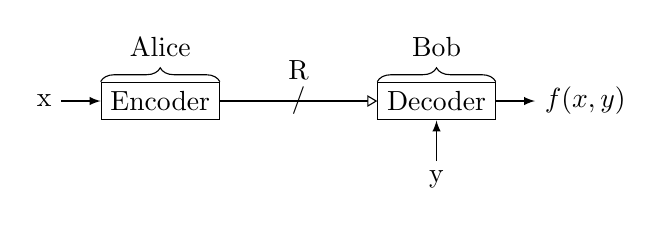
\begin{tikzpicture}[node distance=2cm, >=latex]
    % Nodes
    \node (source) [xshift=-0.5cm] {x};
    \node (encoder) [right=0.5cm of source, rectangle, draw] {Encoder};
    \node (decoder) [right=2cm of encoder, rectangle, draw] {Decoder};
    \node (fxy) [right=0.5cm of decoder] {\( f(x,y) \)};
    
    % Adjusted position of y to 2/3 of the width of the Decoder box.
    \node (y) at ($(decoder.south west)!0.5!(decoder.south east) + (0,-0.75cm)$) {y};
     

    % Connections
    \draw[->] (source) -- (encoder);
    \draw[-{Triangle[fill=white]}] (encoder) -- node[midway,above=0.15cm] {R} node[midway,sloped,anchor=center] {/} (decoder);
    \draw[->] (y) --  ($(decoder.south west)!0.5!(decoder.south east)$);
    \draw[->] (decoder) -- (fxy);
     

    % Braces and annotations
    \draw [decorate,decoration={brace,amplitude=5pt}] (encoder.north west) -- node[above, yshift=0.2cm] {Alice} (encoder.north east);
    \draw [decorate,decoration={brace,amplitude=5pt}] (decoder.north west) -- node[above, yshift=0.2cm] {Bob} (decoder.north east);
     

\end{tikzpicture}
\end{center}
 \caption{Function computation with side information
 \label{fig:func_computing_diag}} 
\end{figure}
In these settings, one is typically interested in the statistics of the data gathered at remote locations, e.g., mean/median/variance, and the like, rather than the data itself. Furthermore, in several of these settings the functions are computed over data that is correlated, e.g., in sensor networks, the readings from different sensors are likely to be similar. In such scenarios, a fundamental question of interest is - {\it ``how to transmit information efficiently so that the function of interest can be computed''.} 


From an information-theoretic perspective, a model that captures several of the inherent subtleties and nuances of the problem is the one depicted in Fig.~\ref{fig:func_computing_diag} and is referred to as the problem of {\it ``function computation with side information''}. Alice observes a source $X$. Bob observes a source $Y$ that is correlated with $X$; $Y$ is referred to throughout as the side information. Bob wishes to compute a function $f(X,Y)$, and for this Alice needs to communicate a certain amount of information to him. The problem is evidently feasible, since Alice can always simply transmit the source $X$. However, determining the minimum amount of information that Alice needs to send is nontrivial in general. This rate depends on the function properties, the correlation structure of $X$ and $Y$ and on the requirements on the recovery of $f(X,Y)$. The case when Bob wants to recover $X$, i.e., when $f(X,Y) = X$, is called ``source coding with side information''.  

The classical version of this problem where Alice communicates classical bits has a long history. The typical setting considers $m$-length blocks of the sources $X_i, Y_i$, for $i \in [m]$ where $[m]= \{1, \dots, m\}$, and the schemes allow the calculation of $f(X_i, Y_i)$ for $i \in [m]$. Suppose that Bob is content with asymptotically error-free reconstruction. This means that the probability that there exists an index in $[m]$ such that the function computation is incorrect can be made arbitrarily small with increasing $m$. In this case, the work of \cite{OrlitskyR_01} provides a precise characterization of the required rate of transmission. In this scenario, for the source coding with side information setting, the solution follows from the Slepian-Wolf theorem \cite{slepian1973noiseless}. On the other hand, if Bob insists on recovering the function computation with zero-error, the problem is significantly more complicated. There are several works in this setting as well, e.g.,
\cite{Witsenhausen_76,FergusonB_75,ahlswede1979coloring,AlonO_95,LinialV89,OrlitskyR_01,KornerO_98,Charpenay_23}. Also, see  Part III of \cite{KornerO_98} for an extensive survey. 


In this work, our focus is on the zero-error version of the function computation with side information. %We study two settings: (i) Classical seting: Alice can transmit classical bits to Bob. Within this setting, two scenarios are considered: (a) Alice uses fixed length codes, and (b) Alice uses variable length codes. (ii) Quantum setting: Alice can transmit quantum states to Bob. 
The study of classical zero-error source coding with side information was initiated in \cite{Witsenhausen_76}. This work introduced the notion of the confusion graph ({\it cf.} Definition \ref{defn:confusion_graph}). Furthermore, it showed that when using fixed length codes, the optimal classical transmission strategy for Alice is to color the confusion graph and transmit the color to Bob. Variable length codes were considered in \cite{AlonO_96} and the corresponding rate was characterized as the chromatic entropy of the confusion graph. Several variants of these problems in the zero-error setting have been examined \cite{CharpenayTR23ITW, CharpenayTR23ISIT, AlonO_96, Shayevitz_14, Malak_22}. %\aditya{CHECK}. \meng{I move the work \cite{Korner_73, KornerL_73} (Korner's graph entropy) to asymptotically error-free part.}
%\aditya{discuss FLC, VLC here}


%\subsection{Background and Related Work}

\subsection{Problem Formulation: Classical and quantum settings}\label{subsec:problem_formulation}
%In this work, we consider the problem of zero-error function computation with side information when there are two parties (see Fig. ~\ref{fig:func_computing_diag}). 
The function computation with side information problem can be formally specified as follows. Alice observes a sequence of independent and identically distributed (i.i.d.)~observations of a random variable $X$ (taking values in a discrete alphabet $\calX$). Bob has access to i.i.d.~observations of a side information random variable $Y$ (taking values in a discrete alphabet $\calY$). $X$ and $Y$ are correlated such that their joint probability mass function (p.m.f.) is $p_{XY}(x,y), x \in \calX, y \in \calY$. Bob seeks to compute a function $f: \calX \times \calY \to \calZ$.  We assume that the channel from Alice to Bob is error-free and can support either classical or quantum transmission depending on the considered scenario.




The aim is to understand the minimum rate at which Alice can communicate information to Bob such that the function computation is successful. We consider $m$-length blocks of the sources $X_i, Y_i$, for $i \in [m]$, and the schemes allow the calculation of $f(X_i, Y_i)$ for $i \in [m]$. We consider $m$-length blocks, since it is often the case that computing multiple instances of the function at the same time allows Alice to send less information ``per'' computation than computing them one by one \cite{shannon1956zero}.

In this work, we consider the {\it zero-error} version of this problem. Thus, for any $m$-instance scheme, we require that Bob should be able to recover $f(X_i, Y_i)$ for all $i \in [m]$.
Suppose that Alice has symbols $x$ and $x'$ such that for all $y$ that occur with joint non-zero likelihood, i.e., $p_{XY}(x,y) > 0$ and $p_{XY}(x',y) > 0$, it holds that $f(x,y) = f(x',y)$. Then, from Bob's perspective, $x$ and $x'$ are equivalent and can be given the same description by Alice. Thus, Alice's symbols that need to be given ``different'' descriptions can be formalized by the following definition \cite{Witsenhausen_76}. 
\begin{definition}
\label{defn:confusion_graph}
{\it $f$-confusion graph.} The $f$-confusion graph of $X$ given $Y$ is a graph $G=(V,E)$ where $V=\calX$ and $(x_1,x_2) \in E$ if there exists $y \in \calY$ such that $p_{XY}(x_1,y) p_{XY}(x_2, y) > 0$ and $f(x_1, y) \neq f(x_2, y)$. 

%Pentagon Figure----------------
\begin{figure}[!t]
\begin{center}
% \begin{tikzpicture}[mystyle/.style={draw,shape=circle,fill=white, inner sep=0pt, minimum size=4pt, label={[anchor=center, label distance=2mm](90+360/\ngon*(#1-1)):#1}}]
% \def\ngon{5}
% \node[draw, regular polygon,regular polygon sides=\ngon,minimum size=3cm] (p) {};

% \foreach\x in {1,...,\ngon}{
%     \node[mystyle=\x] (p\x) at (p.corner \x ){};
% }

\resizebox{0.25\linewidth}{!}{
\begin{tikzpicture}
  \foreach \a in {5}{
    \node [regular polygon, regular polygon sides=\a, minimum size=3cm, draw] at (\a*4,0) (A) {};
    %\foreach \i in {1,...,\a}
    %{%
      %\node [label=90+72*(\i-1):\i, inner sep=1pt] at (A.corner \i) {};
      \node [circle, label=90:0, fill=black, inner sep=3pt] at (A.corner 1) {};
      \node [circle, label=90+72:1, fill=red, inner sep=3pt] at (A.corner 2) {};
      \node [circle, label=90+72*2:2, fill=black, inner sep=3pt] at (A.corner 3) {};
      \node [circle,label=90+72*3:3, fill=red, inner sep=3pt] at (A.corner 4) {};
      \node [circle, label=90+72*4:4, fill=green, inner sep=3pt] at (A.corner 5) {};
    %}
  }
\end{tikzpicture}
}

\end{center}
% \caption{\label{fig:pentagon} {\small $X$ and $Y$ take values in $\{0, \dots, 4\}$ and $Y = X$ or $Y = X+1 \pmod 5$ with equal probability. Bob wants to determine if $X= Y$ or $X \neq Y$. The figure shows the confusion graph for this sceanario. For instance $0$ and $1$ are connected since $p_{XY}(0,1) p_{XY}(1,1) = 1/4 > 0$ and $f(0,1) \neq f(1,1)$. A coloring of this graph can be performed with three colors, so the rate can be $\log_2 3$. However, if we allow computation over two instances, then the rate can be shown to be $\frac{1}{2} \log_2 5$ \cite{witsenhausen1976zero}. Showing that this rate is optimal following from the celebrated result of Lovasz \cite{shannon1956zero}.}}
\vs
\caption{\label{fig:pentagon} {\small The figure shows the $f$-confusion graph $G$ of $f$ with p.m.f. defined in (\ref{eq:corr_prop_eq}). A coloring of $G$ can be performed with three colors. This is shown in the figure with red, black and green. When communicating over one instance, the classical rate can therefore be $\log_2 3$. It can be shown that the graph over two instances $G^{(2)}$ can be colored with five colors. This leads to a per-computation classical rate of $\frac{1}{2} \log_2 5$. This is in fact optimal \cite{Witsenhausen_76,lovasz1979shannon}.}}
\vs
\end{figure}

%-------------------------------

Similarly, if we consider computations over $m$ instances, then we can define the $f$-confusion graph over $m$ instances denoted $G^{(m)}$ analogously. Let $\bfx$ and $\bfy$ denote $m$-length Alice and Bob sequences, respectively. The vertex set corresponds to all $m$-length Alice sequences. $(\bfx_1,\bfx_2) \in E(G^{(m)})$ if there exists $\bfy$ such that $\Pi_{i=1}^m p_{XY}(x_{1i},y_i) p_{XY}(x_{2i}, y_i) > 0$ and there exists $j \in [m]$ such that $f(x_{1j},y_j) \neq f(x_{2j},y_j)$. %The corresponding rate can be obtained as the normalized entropy of the coloring of $G^{(m)}$.
We use shorthand $f^{(m)}(\bfx,\bfy):= \{f(x_i,y_i)\}_{i=1}^m$, and $p_{\bfX\bfY}(\bfx,\bfy)= \prod_{i=1}^mp_{XY}(x_i,y_i)$.
\end{definition} 

\begin{example}
Consider a scenario where  $X$ and $Y$ take values in $\{0, 1, \dots, 4\}$ and are correlated such that 
    \begin{align}
       p_{XY}(x,y)  &= \begin{cases}
            \frac{1}{10}, \text{~if~} y=x\text{~or~}y=(x+1)\Mod 5,\\
            0,\text{~otherwise.}
        \end{cases} \label{eq:corr_prop_eq}
    \end{align}
Suppose that Bob wishes to compute the equality function, i.e., $f(X,Y) = 1$ if $X=Y$ and $f(X,Y) =0$ if $X\ne Y$. We observe that Alice's symbols $0$ and $1$ are connected since $p_{XY}(0,1) p_{XY}(1,1) = 1/100 > 0$ and $f(0,1) \neq f(1,1)$; the reasoning for the other edges is similar. It can be observed that this $f$-confusion graph is a pentagon (see Fig. \ref{fig:pentagon}).   
\end{example}

%revised
In general, the structure of the $m$-instance confusion graph $G^{(m)}$ can be quite complicated. Graph products are classes of graphs that are more structured and extensively studied \cite{HammackGraphProduct}. It turns out that studying graph products allows us to also characterize general $m$-instance confusion graphs at some level.
In particular, we will deal extensively with the strong product and the OR product of graphs. These are defined below.
%The structure of general multiple-instance $f$-confusion graph seems intractable.  One question we answer is when an $f$-confusion graph can be written as a graph product. We will deal extensively with graph products.  %gives two-fold strong product and OR product  of $G$, and  strong product and OR product are defined below. 
%\aditya{Will reword this para based on discussion with Ruoyu.}
%
%Furthermore, we will deal extensive with the following graph products that generate a new graph from two graphs $G$ and $H$.
%

\begin{definition}\label{defn:AND_product_OR_product}
     The strong product of $G$ and $H$, denoted $G\boxtimes H$, has vertex set $V(G)\times V(H)$. $\big( (u_1,v_1),(u_2,v_2) \big )\in E(G\boxtimes H)$ if and only if
    \begin{align*}
        & \big (u_1=u_2\text{ and }(v_1,v_2)\in E(H)\big )\text{ or}\\
        & \big ((u_1,u_2)\in E(G)\text{ and }v_1=v_2\big )\text{ or}\\
        & \big ((u_1,u_2)\in E(G)\text{ and }(v_1,v_2)\in E(H)\big ).
    \end{align*}
    The $m$-fold strong product is written as $G^{\boxtimes m} := \underbrace{G\boxtimes G\boxtimes \dots \boxtimes G}_{m\text{ times}}.$
    
\noindent The OR product of $G$ and $H$, denoted $G\lor H$, has vertex set $V(G)\times V(H)$. $\big((u_1,v_1),(u_2,v_2)\big)\in E(G\lor H)$ if and only if 
    \begin{align*} 
            (v_1,v_2)\in E(H)&\text{ if }u_1=u_2,\\
            (u_1,u_2)\in E(G)&\text{ if }v_1=v_2,\\
            (u_1,u_2)\in E(G) \text{ or }(v_1,v_2)\in E(H)&\text{ if }u_1\ne u_2\text{ and }v_1\ne v_2. 
    \end{align*}
    The $m$-fold OR product is written as $G^{\lor m} :=\underbrace{ G\lor G\lor \dots \lor G}_{m\text{ times}}.$
\end{definition}


\begin{figure}[t]
    \centering
    \scalebox{1}{%

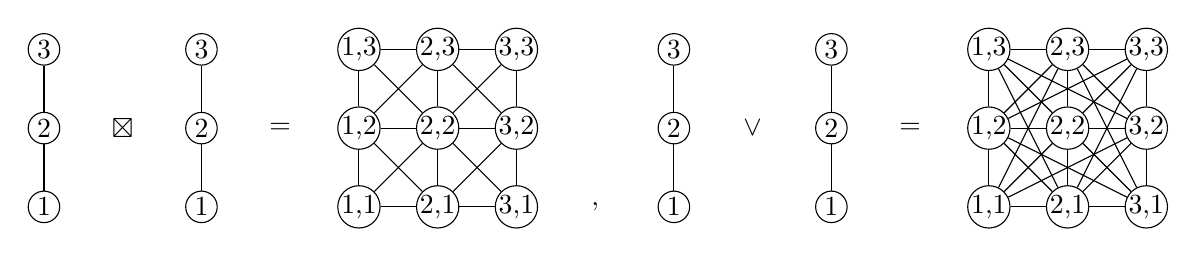
\begin{tikzpicture} 
[
  node distance=0.5cm,
  every node/.style={circle, draw, minimum size=4mm, inner sep=0pt, font = \normalsize},
  every edge/.style={draw, -} 
]

\node[draw=none] (times) at (-2,2) {$\boxtimes$}; 

\node[draw=black] (001) at (-3,1) {1};
\node[draw=black] (002) at (-3,2) {2};
\node[draw=black] (003) at (-3,3) {3}; 

\node[draw=black] (01) at (-1,1) {1};
\node[draw=black] (02) at (-1,2) {2};
\node[draw=black] (03) at (-1,3) {3}; 

\node[draw=none] (equal) at (0,2) {$=$}; 


\node[draw=black] (11) at (1,1) {1,1};
\node[draw=black] (12) at (1,2) {1,2};
\node[draw=black] (13) at (1,3) {1,3}; 

\node[draw=black] (21) at (2,1) {2,1};
\node[draw=black] (22) at (2,2) {2,2};
\node[draw=black] (23) at (2,3) {2,3}; 

\node[draw=black] (31) at (3,1) {3,1};
\node[draw=black] (32) at (3,2) {3,2};
\node[draw=black] (33) at (3,3) {3,3}; 

 

\draw (01) edge (02);
\draw (02) edge (03); 

\draw (11) edge (12);
\draw (12) edge (13); 

\draw (21) edge (22);
\draw (22) edge (23); 

\draw (31) edge (32);
\draw (32) edge (33); 

\draw (001) edge (002);
\draw (002) edge (003); 


\draw (11) edge (21);
\draw (21) edge (31); 

\draw (12) edge (22);
\draw (22) edge (32); 

\draw (13) edge (23);
\draw (23) edge (33); 


\draw (11) edge (22);
\draw (21) edge (32); 

\draw (12) edge (23);
\draw (22) edge (33); 

\draw (12) edge (21);
\draw (22) edge (31); 

\draw (13) edge (22);
\draw (23) edge (32); 


\node[draw=none] (comma) at (4,1) {$,$}; 

\node[draw=none] (times) at (6,2) {$\lor$}; 

\node[draw=black] (661) at (5,1) {1};
\node[draw=black] (662) at (5,2) {2};
\node[draw=black] (663) at (5,3) {3}; 

\node[draw=black] (61) at (7,1) {1};
\node[draw=black] (62) at (7,2) {2};
\node[draw=black] (63) at (7,3) {3}; 

\node[draw=none] (equal) at (8,2) {$=$}; 


\node[draw=black] (71) at (9,1) {1,1};
\node[draw=black] (72) at (9,2) {1,2};
\node[draw=black] (73) at (9,3) {1,3}; 

\node[draw=black] (81) at (10,1) {2,1};
\node[draw=black] (82) at (10,2) {2,2};
\node[draw=black] (83) at (10,3) {2,3}; 

\node[draw=black] (91) at (11,1) {3,1};
\node[draw=black] (92) at (11,2) {3,2};
\node[draw=black] (93) at (11,3) {3,3}; 

 

\draw (61) edge (62);
\draw (62) edge (63); 

\draw (71) edge (72);
\draw (72) edge (73); 

\draw (81) edge (82);
\draw (82) edge (83); 

\draw (91) edge (92);
\draw (92) edge (93); 

\draw (661) edge (662);
\draw (662) edge (663); 


\draw (71) edge (81);
\draw (81) edge (91); 


\draw (72) edge (82);
\draw (82) edge (92); 

\draw (73) edge (83);
\draw (83) edge (93); 


\draw (71) edge (82);
\draw (81) edge (92); 


\draw (72) edge (83);
\draw (82) edge (93); 

\draw (72) edge (81);
\draw (82) edge (91); 

\draw (73) edge (82);
\draw (83) edge (92); 


\draw (71) edge (92);
\draw (71) edge (83); 

\draw (93) edge (81);
\draw (73) edge (81); 



\draw (91) edge (72);
\draw (91) edge (83); 

\draw (73) edge (92);
\draw (93) edge (72); 

\end{tikzpicture}
    }
    \caption{Strong product and OR product of $G$ with itself where $G$ is a path of two edges.}
    \label{fig:strong_or_product_P3}
\end{figure} 

\noindent Examples of strong and OR products appear in Fig. \ref{fig:strong_or_product_P3}.
%The aim is to understand the minimum rate at which Alice can communicate information to Bob such that the function computation is successful with probability 1, i.e., the probability of error is zero. When Alice seeks to communicate the source $X$ to Bob, i.e., when $f(X,Y) = X$, the problem is referred to as source coding with side information.

%The typical setting considers $m$-length blocks of the sources $X_i, Y_i$, for $i \in [m]$ where $[m]= \{1, \dots, m\}$, and the schemes allow the calculation of $f(X_i, Y_i)$ for $i \in [m]$. We consider $m$-length blocks, since it is often the case that computing multiple instances of the function at the same time allows Alice to send less information ``per'' computation than computing them one by one \cite{shannon1956zero}. The problem can formally be posed as follows.








 %There are two different dimensions to this problem. 

% \meng{Additional background}
% Alice may encode her inputs $(X_i)_{i\in[m]}$ with different  communication cost, i.e. the length of bits transmitted may vary in $(X_i)_{i\in[m]}$. We assume Bob knows where message ends and define the cost of a protocol is the longest bits among all possible $(X_i)_{i\in[m]}$. \meng{Define this way because it is a simple way to formulate the problem.} Under this setting, the problem can be formulated using graph-theoretic approach \cite{Witsenhausen_76}. Under classical and quantum communication, the communication cost corresponds to the chromatic number and "orthogonal rank" of a "confusion graph" respectively. 

% The structure of the "confusion graph" under multiple-instance is  crucial for determination of the rate. When "confusion graph" is a "$m$-fold graph OR product", the classical communication rate has a simple expression in terms of one-shot "confusion graph". To the best of our knowledge, all other cases do not have such a simple expression. We ask the question whether a simple condition can be derived such that the multiple-instance "confusion graph" can be written as some graph products.

% Compared with classical communication, it is natural to ask whether quantum communication have less communication cost. This problem can be studied in two scenario. The first scenario is that the function only needs to be computed for one-instance. This scenario is the one-way communication complexity problem and has been extensively studied \meng{cite some survey}. The second scenario is 
% that the function needs to be computed for multiple-instances. One motivation of this paper is to understand how the quantum advantage changes as the number of instances increases and how this change varies under different "confusion graphs".

% \aditya{General comment - replace all instances of such that  with such that}\meng{Done}

%revised
In this work, we examine the zero-error function computation with side information problem under three different settings. In the first setting, Alice transmits   fixed length classical codes to Bob,  (i.e., the setting of \cite{Witsenhausen_76}). In the second setting, Alice transmits   variable length classical codes to Bob,  (i.e., the setting of restricted inputs in  \cite{AlonO_96}). In the third setting, Alice transmits fixed dimension quantum states to Bob. %We utilize the definition of the $m$-instance $f$-confusion graph $G^{(m)}$ below. We will often need to refer to the following definition of the coloring of a graph. 
%\aditya{Can we refer to any work that states that variable length quantum codes are hard to define or consider?}
\begin{definition}
    Let $G=(V,E)$ be a graph. A $k$-coloring of $G$ is a labeling $f:V\mapsto S$, where $S$ is a set of $k$ elements, such that adjacent vertices have different labels. The chromatic number $\chi(G)$ is the minimum $k$ such that there exists a $k$-coloring of $G$.
\end{definition}

%revised
\subsubsection{\bf Fixed Length Classical Code (FLC) Setting}

%\subsection{Problem Formulation: Classical and quantum settings} 

%In the subsequent discussion in this section, let $G = (V, E)$ represent the $f$-confusion graph of $X$ given $Y$ and $G^{(m)} = (V^{(m)}, E^{(m)})$ the corresponding $m$-instance version ({\it cf.} Definition \ref{defn:confusion_graph}).

%Pentagon Figure----------------
%\input{figures/function_computing_diagram}
%-------------------------------

In the fixed length classical code setting, based on the work of Witsenhausen \cite{Witsenhausen_76}, it can be observed that Alice's strategy corresponds to coloring $G^{(m)}$ with the fewest possible colors and transmitting the color of her realization\cite{Witsenhausen_76}. Thus, the FLC rate is defined as follows. %\cite{Witsenhausen_76,FergusonB_75,ahlswede1979coloring}. %\aditya{For completeness, let us keep a proof of this also somewhere}
%revised
\begin{definition} 
\label{defn:witsenhausen_classical_rate} {\it Optimal rate in the FLC setting.} The FLC rate is given by 
\begin{align*}
    R_{\text{FLC}} &= \lim_{m \to \infty} \frac{\log_2 \chi(G^{(m)})}{m} = \inf_m  \frac{\log_2 \chi(G^{(m)})}{m}.
\end{align*}
\end{definition}
The second equality above, follows from the sub-additivity of $\log_2 \chi(G^{(m)})$ \cite{NayakTR06}. In the sequel, we will use $R_{\text{FLC}}^{(1)} = \log_2 \chi(G)$ to denote the single-instance rate. %\aditya{Specify log to base-2}

% , which based on the aboive
% we will often refer to $\log \chi(G)$ as the single-instance rate and $R_{\text{classical}}$ as the asymptotic rate.

%revised
\subsubsection{\bf Variable Length Classical Code (VLC) Setting} \label{subsubsec:VLC_setting}

%In order to discuss the setting of variable-length codes, we recapitulate some well-known definitions within classical source coding.



Let $\{0, 1, \dots, D-1\}$ be a $D$-ary alphabet from which the symbols in a variable length code are chosen, and let $ \{0,\dots, D-1\}^*$ denote the set of all finite-length strings from $\{0, 1, \dots, D-1\}$. A graph $H$  is said to be an induced subgraph of $G$ if its vertex set $V(H)$ is a subset of $V(G)$  and edge set $E(H)$ consists of edges in $E(G)$ whose two endpoints are in $V(H)$. For $\bfy$ of length-$m$, let $G^{(m)}_\bfy$ denote the induced subgraph of $G^{(m)}$ consisting of the subset of $\bfx$ vertices that occur along with $\bfy$ with strictly positive probability, i.e., $V(G^{(m)}_\bfy) = \{\bfx:\bfx\text{ such that }p_{\bfX\bfY}(\bfx,\bfy)>0\}$ and $E(G^{(m)}_\bfy) = \{(\bfx_1,\bfx_2):(\bfx_1,\bfx_2)\in E(G^{(m)})\text{ and }\bfx_1,\bfx_2\in V(G^{(m)}_\bfy)\}$. %\meng{Give a correct definition of induced subgraph and $G^(m)_y$}





%The "restricted inputs" problem in \cite{AlonO_96} can be considered a special case of our problem by setting  $f^{(m)}(\bfx,\bfy)=\bfx$. For the general function $f^{(m)}(\bfx,\bfy)$, we require that Bob should be able to recover $f^{(m)}(\bfx,\bfy)$ from the message received and his $\bfy$. 





%Let $m\in \bbN$ and $\bfX,\bfY$ be length-$m$ i.i.d. sequences of $X,Y$s. 

%In the VLC setting, we define the requirements on the zero-error protocol as follows.
\begin{definition}{\it Non-singular Code.} \label{def:ns_code}
A $m$-instance variable length code consists of an encoding function $\phi_{e}:V(G^{(m)}) \mapsto \{0,\dots, D-1\}^*$ such that $\phi_e$ is a coloring of $G^{(m)}_\bfy$ for all $\bfy$. This means that if $(\bfx_1,\bfx_2)$ is an edge in $G^{(m)}_\bfy$, then $\phi_{e}(\bfx_1) \neq \phi_{e}(\bfx_2)$. In this case, we call the variable length code, non-singular.
\end{definition} 

It is not too hard to see that a non-singular variable length code as described above corresponds to a coloring of the $m$-instance graph $G^{(m)}$. Indeed, $(\bfx_1, \bfx_2) \in E(G^{(m)})$ then there exists a $\bfy$ such that $(\bfx_1, \bfx_2) \in E(G^{(m)}_\bfy)$ and hence $\phi_e(\bfx_1) \neq \phi_e(\bfx_2)$. On the other hand, suppose that we consider a variable length non-singular source code as defined in \cite{CoverT05} (Chapter 5), that encodes a given coloring of $G^{(m)}$. Then, by setting $\phi_e(\bfx)$ to be the encoding of its color, we observe that we arrive at a valid non-singular variable length code for our problem. 

\begin{definition}{\it Prefix-free code.} \label{def:pf_code}
Consider a $m$-instance non-singular variable length code with encoding function $\phi_e: V(G^{(m)}) \mapsto \{0, \dots, D-1\}^*$.
Let $\phi_e(G^{(m)}_\bfy) \triangleq \{\phi_e(\bfx):\text{~where~} \bfx \in V( G^{(m)}_\bfy)\}$ denote the subset of all encodings corresponding to vertices in $G^{(m)}_\bfy$, i.e., $\phi_e(G^{(m)}_\bfy)$ is the image of the map $\phi_e(\cdot)$ when $\bfx$ is restricted to $V( G^{(m)}_\bfy)$. Suppose that for all $\bfy$ we have the following property. Let $\zeta_i \in \phi_e(G^{(m)}_\bfy), i =1,2$ such that $\zeta_1 \neq \zeta_2$. Then, we have that $\zeta_1$ is not a prefix of $\zeta_2$. In this case, we call the variable length code, prefix-free. 
\end{definition}  %\aditya{CHeck this definition} \meng{Done}  

\begin{remark}\label{remark:AlonO_prefix-free}
In \cite{AlonO_96}, the authors define a prefix-free variable length code for the problem of source coding with side information, where they enforce that $\phi_e(\bfx_1)$ is not a prefix of $\phi_e(\bfx_2)$ if $(\bfx_1, \bfx_2) \in E^{(m)}$. As discussed in Section \ref{sec:VLC_rate_graph_entropy}, Example \ref{example:C5_VLC}, this definition is not appropriate for the general function computation problem.
%
%In the general function computation context, the above definition is the appropriate one to use. We will discuss this in Sec. \ref{sec:VLC_rate_graph_entropy} Example \ref{example:C5_VLC}.  
\end{remark} 


\textbf{Extension of a code:} Consider a prefix-free variable length code for a given value of $m$. Then, this code can be extended to all multiples of $m$ by simply concatenating the encodings; this is referred to as an extension of the original code (Chapter 5 of \cite{CoverT05}). For example, the encoding for a length $2m$ vector $[\bfx~ \bfx']$ will be the concatenation $\phi_e(\bfx)\phi_e(\bfx')$. This implies, for instance, that a prefix-free variable length code for $m=1$ can be employed as a code for arbitrary $m$ by extension, such that Bob can instantaneously decode $\phi_e(x_i), i = 1, \dots, m$ from the string $\phi_e(x_1)~\phi_e(x_2)~\dots~\phi_e(x_m)$.

On the other hand, a non-singular code for a given $m$ cannot necessarily be extended so that it is even uniquely decodable \cite{CoverT05} (see Example \ref{example:C5_VLC} in Section \ref{sec:VLC_rate_graph_entropy}). For this reason, henceforth, we will only consider prefix-free variable length codes and define rates accordingly.



%Our definition of a prefix-free variable length protocol, allows for instantaneous decoding by Bob when he receives a concatenated seqe

%\aditya{Should we define both non-singular and prefix-free rates?}

%\aditya{Need to justify why we only deal with prefix-free rate}
\begin{definition}{\it Optimal Rate in VLC setting.} \label{def:VLC_rate}
Consider a prefix-free variable length code for our problem. Let  $|\phi_e(\bfx)|$ denote the length of the encoded $D$-ary  string corresponding to $\phi_e(\bfx)$. Then, the rate of this code is defined as $R_{VLC}^{(m)} \triangleq \frac{1}{m}\sum_{\bfx}p_{\bfX}(\bfx)|\phi_e(\bfx)|$ where $p_{\bfX}(\cdot)$ is the marginal distribution of $\bfX$.
The optimal rate is defined as
\begin{align}
    R_{VLC} &=  \inf_m \min_{\phi_e} R^{(m)}_{VLC},
\end{align}
%\aditya{put in sub-additivity argument}\meng{Done}
where $\min_{\phi_e} R^{(m)}_{VLC}$ is the rate of the optimal $m$-instance encoding. %$\min_{\phi_e} R^{(m+n)}_{VLC}\le \min_{\phi_e} R^{(m)}_{VLC}+ \min_{\phi_e} R^{(n)}_{VLC}$ holds. Fix  encodings $\phi_{e},\phi_{e}'$ for $G^{(m)},G^{(n)}$ respectively. Let $\bfx=(\bfx_1,\bfx_2)\in \calX^{(m+n)}$ where $ \bfx_1 \in \calX^{m }),\bfx_2 \in \calX^{n })$ respectively. We can concatenate encodings $\phi_{e}(\bfx_1)\phi_{e}'(\bfx_2)$. This results in a $(m+n)$-instance encoding. 
\end{definition}



%\aditya{Need a proof that this a valid VLC protocol - put in check}
%\aditya{Also, need to explain the differences that occur that happen in the cases and why only considering the confusion graph is not enough.}\meng{I guess Example 2 works}
%For each $m$, denote  $R^m_{VLC}$ the minimum $R_m$ such that   there exists an $(m, R_m)$ VLC protocol. The optimal
%rate is denoted by $R^{\star}_{VLC}  = \inf_m R^m_{VLC} $. 
%\begin{example}
%Alice is given numbers $x\in \{1,2,3,4\}$  with equal probability, i.e. $\forall x, p(x)=1/4,$ and Bob does not know any side information ($\calY=\emptyset$), and Bob wants to know the parity of $x$, i.e. $f(1)=f(3)=O,f(2)=f(4)=E$ ($O,E$ stand for odd and even respectively). The confusion graph is a cycle with 4 vertices. Suppose  Alice uses the encoding in Fig. \ref{fig:c4_encoding} where adjacent vertices have prefix-free encodings; this meets the criterion of \cite{AlonO_96}. While this is not an optimal encoding, it serves to demonstrate the relevant point.  
%\begin{figure}[h]
%    \centering
%    \input{figures/Fig_C4_example}
%    \caption{Encoding of Alice}
%    \label{fig:c4_encoding}
%\end{figure}
%Since adjacent vertices are not prefix of each other, this  is an encoding that meets the criterion of \cite{AlonO_96}. 
%In the single-instance case, this is a valid protocol. However, if we consider extension of the protocol, the encoding causes error. Consider the following three cases. \aditya{can be shortened}\meng{shortened}
%\begin{enumerate}
%    \item Alice has 2 instances: $(x_1,x_2)=(1,2)$. She uses extension of $\phi_e$ and sends $(\phi_e(x_1),\phi_e(x_2) ) = 101$. The function value should be $(f(1),f(2) )=(O,E )$.
%    \item Alice has 2 instances: $(x_1,x_2)=(3,1)$. She uses extension of $\phi_e$ and sends $(\phi_e(x_1),\phi_e(x_2) ) = 101$. The function value should be $(f(3),f(1) )=(O,O )$.
%\end{enumerate}
%Each of  2 cases has a distinct function value, but the messages sent to Bob are all the same, i.e. "101". Therefore, Bob cannot distinguish the case, and cannot have zero-error decoding. 

%    \aditya{Include example that shows that ALON-ORLITSKY encoding may fail for our case.}\meng{added}
%\end{example}

%\aditya{Should we move the stuff below to the actual section?}\meng{we moved}


% \begin{remark}
% In Definition \ref{def:VLC_rate}, the  constraint 2) guarantees that Bob  knows when the massage ends given his $\bfy$. Other versions of the  constraint 2) were considered in  \cite{CharpenayTR23ISIT} and \cite{AlonO_96} with the same asymptotic optimal rates.
% \end{remark}
\begin{remark}\label{remark:VLC_depends_on_p_X}
    Unlike the fixed length code rate, the variable length code rate depends on the marginal distribution $p_X(\cdot)$ of the random variable $X$.  %\meng{Should we remove this remark?}
\end{remark}
\subsubsection{\bf Quantum Setting} 
The following notions are standard within quantum information theory (see \cite{wilde_17}). A quantum bit (qubit) or more generally a qudit represented by $\ket{\psi}$ (Dirac's bra-ket notation) is a unit-norm column vector in a complex Hilbert space $\calH$. A closed quantum system evolves only via unitary transformations $U$, i.e., $\ket{\psi} \mapsto U \ket{\psi}$, where $U U^\dagger = U^\dagger U = I$ ($\dagger$ denotes conjugate transpose). Two qudits $\ket{\psi_1} \in \calH_A$ and $\ket{\psi_2} \in \calH_B$ lie in the (composite) tensor product space $\calH_A \otimes \calH_B$. Quantum states can be ``pure'' in which case they can be represented as vectors. Quantum states can also be mixed, e.g., pure state $\ket{\psi_x}$ may be prepared with probability $p_X(x)$. For a Hilbert space $\calH$, let $\calL(\calH)$ denote the set of linear operators from $\calH$ to itself; treated as matrices, these are square matrices. When states are mixed, the description of the state is given by a density operator in $\calL(\calH)$,  $\rho_X = \sum_{x \in \calX} p_X(x) \ket{\psi_x} \bra{\psi_x}$. A density operator (or quantum state) is a positive Hermitian operator\footnote{A positive operator $A$ over a complex Hilbert space, denoted $A \succeq 0$ is Hermitian, i.e., $A = A^\dagger$ and has non-negative eigenvalues. Treated as a matrix, it is a Hermitian, positive semi-definite matrix.} with unit-trace. The density operator of a pure state $\ket{\psi_x}$ is written as $\ket{\psi_x}\bra{\psi_x}.$ A quantum measurement is a fundamental operation by which information can be extracted from a quantum system. While there are many different measurement formalisms, here we discuss the positive operator-valued measure (POVM) measurements which are relevant to our work. These are specified by a set of positive operators $\{\Lambda_j\}_{j=1}^{k}$ where $\Lambda_j \succeq 0$ and $\sum_{j=1}^k \Lambda_j = I$ 
 ($I$ denotes the identity operator). The probability of obtaining measurement value $i$ is given by $\Tr \left(\Lambda_i \rho_X \right)$ for $i \in [k]$. Quantum states $\rho$ and $\sigma$ are said to be orthogonal, denoted $\rho \perp \sigma$ if $\Tr (\rho^{\dagger} \sigma) = 0$. This is equivalent to $\rho$ and $\sigma$ having orthogonal supports\footnote{The support of an operator is the orthogonal complement of its kernel. For Hermitian operators (as we consider) the support is its image.}. Two  quantum states $\rho$ and $\sigma$ are said to be perfectly distinguishable if there exists a POVM $\{\Lambda_j\}_{j=1}^{k}$ such that $\Tr \left(\Lambda_i \rho \right)\Tr \left(\Lambda_i \sigma \right) = 0$ for $i \in [k]$, i.e., there exists a POVM $\{\Lambda_j\}_{j=1}^{k}$ which distinguishes $\rho$ and $\sigma$ with zero-error. Such a POVM exists if and only if $\rho$ and $\sigma$ are orthogonal \cite{MEDEIROSD05}. Note that for this case $k=2$ suffices. However, in our discussion later, we need to perfectly distinguish multiple states. 
 
 
 %\meng{Added what means "two states are  perfectly distinguishable"} \aditya{Need to discuss} 
 
 %For composite systems, we consider positive, unit-trace operators that act on the tensor product space $\calH_A \otimes \calH_B$, e.g. state $\rho_{AB} \in \calL(\calH_A \otimes \calH_B)$ is a density operator that lies in the set of linear operators mapping $\calH_A \otimes \calH_B$ to itself. In this case, the state on subsystem $A$, denoted $\rho_A$ is given by the partial trace operator $\Tr_{B} \left(\rho_{AB}\right)$. Quantum states on composite systems can be entangled (see \cite{nielsenC11} for a detailed discussion). For a pure state $\ket{\psi}_{AB}$ on $\calH_A \otimes \calH_B$, this means that $\ket{\psi}_{AB}$ cannot be expressed as $\ket{\sigma}_{A} \otimes \ket{\sigma}_{B}$ for pure states $\ket{\sigma}_A$ and $\ket{\sigma}_B$ on spaces $\calH_A$ and, $\calH_B$ respectively. For instance, the maximally entangled state on the composite system $AB$ can be represented as $\ket{\Phi}_{AB} = \frac{1}{\sqrt{2}} \left(\ket{00}_{AB} + \ket{11}_{AB} \right)$. The judicious usage of entangled states enables protocols \cite{nielsenC11, wilde_2013} such as (i) superdense coding which allows two classical bits to be communicated with one qubit transmission, and (ii) quantum teleportation which allows the transmission of a qubit by only transmitting two classical bits.






Suppose that Alice and Bob have $m$-length sequences $\bfx$ and $\bfy$ and Alice communicates to Bob through an error-free quantum channel that supports the transmission of operators on $\calH$. The quantum code for our problem setting operates as follows.
\begin{itemize}[leftmargin=2mm]
    \item Alice picks a quantum state $\rho_\bfx \in \calL(\calH)$ (where $\dim \calH = d$), that depends on the sequence $\bfx$ and transmits it to Bob.  
    \item Bob performs a POVM measurement\cite[pg. 134]{wilde_17} on the received state. The POVM, which is dependent on $\bfy$, is specified by $\{\Lambda^\bfz_{f(\cdot,\cdot), \bfy}\}_{\bfz \in \calZ^m}$, where the indices $\bfz$ are measurement results and the matrices $\Lambda^\bfz_{f(\cdot,\cdot), \bfy}$ are positive semi-definite matrices that sum to the identity, i.e., $\Lambda^\bfz_{f(\cdot,\cdot), \bfy} \succeq 0$, for $\bfz \in \calZ^m$, and $\sum_{\bfz \in \calZ^m}  \Lambda^\bfz_{f(\cdot,\cdot), \bfy} = I$.
    
    % \begin{align*}
    %     \Lambda^\bfz_{f(\cdot,\cdot), \bfy} \succeq 0, \text{~for~} \bfz \in \calZ^m, \quad \text{~and} \quad 
    %     \sum_{\bfz \in \calZ^m}  \Lambda^\bfz_{f(\cdot,\cdot), \bfy} = I.
    % \end{align*}


    % \begin{align*}
    %     \Lambda^\bfz_{f(\cdot,\cdot), \bfy} &\succeq 0, \text{~for~} \bfz \in \calZ^m, \text{~and},\\
    %     \sum_{\bfz \in \calZ^m}  \Lambda^\bfz_{f(\cdot,\cdot), \bfy} &= I.
    % \end{align*}
\end{itemize}
%We note that Bob's measurement depends on the function $f(\cdot, \cdot)$ and his observed sequence $\bfy$.
The code is deemed successful if $z_i = f(x_i, y_i)$, for $i \in \{ 1, \dots, m\}$ for all possible pairs $(\bfx, \bfy)$. %\meng{maybe mention $z_i$ is measurement result.}
 Alice's rate of transmission is defined as $\frac{1}{m} \log_2 d$.



It can be shown ({\it cf.} Section \ref{sec:orth_rep}), that this code is zero-error if and only if for $(\bfx, \bfx') \in G^{(m)}$ then $\rho_\bfx \perp \rho_{\bfx'}$. If this condition is satisfied, depending on the $\bfy$ sequence observed by Bob, it can be shown that he can prepare the measurement such that   the function value is recovered with zero error. Furthermore, Alice needs to find the suitable set of states in as small of a dimension $d$ as possible, so that the task can be achieved by transmitting the fewest number of quantum bits. The quantum rate is defined formally in Section \ref{sec:orth_rep} (Theorem \ref{thm:witsenhausen_quantum_rate}). As in the classical case, we make a distinction between the single-instance rate and the asymptotic rate.

We point out that the classical FLC code can be considered as an instance of the proposed quantum code, simply by operating in a large enough vector space and labeling the nodes of the $f$-confusion graph by canonical basis vectors (binary vectors with all components zero except one). However, considering general unit-norm vectors provides much more flexibility and therefore the dimension $d$ in which we need to operate in, can be lower; concrete examples can be found ({\it cf.} Section \ref{sec:analysis_bahavior_quantum_advantage}).

%\meng{Added an explanation that we don't consider quantum VLC} 
We emphasize that there are significant difficulties with defining variable length quantum codes. In particular, as pointed out in \cite{BraunsteinFGH98}, determining the quantum message boundaries will itself require measurement, which will, in general, destroy superposition. Thus, in this work we do not consider variable length quantum codes. %\aditya{CHECK}\meng{Fine for me.}
%We do not consider a quantum version of variable-length code, because it is much more difficult.  Bob are forbidden to measure the length of the message, because the measurement may destroy the superposition of the quantum state. As a consequence, Bob does not even know where the message ends. See \cite{BraunsteinFGH98} for more difficulties in building a quantum VLC.
 


\subsection{Related work}\label{subsec:related_work}
A natural conditional entropy defined on the confusion graph provides the precise rate characterization for function computation with side information when the computation is only required to be lossless, i.e., the distortion is asymptotically vanishing; it is not a zero-error scenario \cite{OrlitskyR_01}. The Slepian-Wolf theorem \cite{slepian1973noiseless} addresses the case of source coding with side information.

The exhaustive survey paper \cite{KornerO_98} overviews several aspects of classical zero-error information theory. We first discuss the case of  classical source coding with side information. 
Witsenhausen \cite{Witsenhausen_76} considered the usage of fixed length codes in this setting and showed the optimal rate could be analyzed by considering the chromatic number of the corresponding $f$-confusion graph. We note here that in general, a single-letter characterization of the optimal rate is not available. 
Alon and Orlitsky  \cite{AlonO_96} considered variable length codes and related the rate characterization to an appropriately defined chromatic entropy of $f$-confusion graph. It is well-known that the multiple instance rate can be much less than the single instance rate \cite{KornerO_98}. For instance, it can be observed that the $f$-confusion graph in the pentagon example ({\it cf.} Fig. \ref{fig:pentagon}) can be colored with three colors so that the rate can be $\log_2 3$. However, if we allow computation over two instances, then it can be shown that the corresponding graph can be colored with five colors so that the rate equals $\frac{1}{2} \log_2 5$ \cite{Witsenhausen_76,lovasz1979shannon}. It turns out that this rate is optimal for this problem; this follows from a celebrated result of Lov{\'a}sz\cite{lovasz1979shannon}.  Orlitsky \cite{orlitsky_worst_case90} also considered the case of interactive communication between Alice and Bob. For the variable length codes, \cite{KoulgiTRR_03} expresses the optimal rate as complementary graph entropy of $f$-confusion graph. While this quantity is still hard to compute in general, \cite{CharpenayTR23ISIT} consider certain cases where it can actually be computed. Reference \cite{CharpenayTR23ITW}, considers a zero-error function computation model where side information is also available at the encoder. For this model, under specific conditions on the joint p.m.f. and Alice's side information, they derive a single-letter characterization of the optimal rate.

Function computation has also been studied in the scenario where both $X$ and $Y$ are transmitted by remote entities and Bob seeks to compute $f(X,Y)$ with asymptotically vanishing error. The work of \cite{HanK87} determined a necessary and sufficient condition on $f(\cdot, \cdot)$ such that the optimal rate region coincides with the Slepian-Wolf region. In these scenarios, structured codes often outperform random codes, as pointed out in \cite{KornerM79} for the problem of recreating the modulo-2 sum of binary sources. The work of \cite{NazerG07, wilson_etal10} consider function computation over multiple-access channels. More recently, function computation over quantum many-to-one networks has been considered in \cite{AllaixLYPHCJ24}.


% %In \cite{KrithivasanP09}, lattice coding is shown to outperform Berger-Tung coding \cite{BergerHOSW79}.  
% The structure of function can be utilized to reduce communication . Physical realization of the network (wireless, cable, optical fiber etc.) \cite{NazerG07, AhlswedeCL06, MillerBWK10, GoldenbaumBS12} as well as the structure of function \cite{KornerM79,JiaJ21} can be utilized to reduce communication. Structure of the network (MAC, directed graph) is crucial for the rate region \cite{NazerG07,LiYN03}. Analogs of MAC in quantum network are also considered \cite{AllaixLYPHCJ24,HayashiINRY07,YaoJ24}. \meng{related work for MAC CHECK}


There have been a few works that consider quantum generalizations of classical zero-error problems. The work of \cite{cubitt2010improving} considers communicating with zero error over a noisy discrete memoryless channel (DMC), denoted $W$ in the presence of shared entanglement between the source and the terminal. Let $C_0(W)$ and $C_{SE}(W)$ denote the zero-error capacity of the channel in the absence and in the presence of shared entanglement, respectively. Their work demonstrates that there exist DMCs such that $C_0(W) < C_{SE}(W)$; these are constructed by leveraging Kochen-Specker sets \cite{held2009kochen}. This is rather interesting since the work of Bennett et al. \cite{bennett2002entanglement} shows that the presence of shared entanglement does not increase the capacity of a classical channel when considering asymptotically error-free communication. Following this work, there were several works that considered entanglement-assisted zero-error source-channel coding. The work of \cite{BrietBL_15} considers shared entanglement, but the sources and channels are still classical. The work of Stahlke \cite{stahlke2015quantum} considers quantum sources and quantum channels. However, none of these works consider general functions.% \aditya{CHECK} \meng{Done, this is true}.


Prior work that is most closely related to our work includes \cite{BuhrmanCW_98, GavinskyKKRd_07, Bar-YossefJK08}. For function computation, these works demonstrate that there exists an exponential separation between the classical and the quantum rate. However, these results are for the single-instance case, i.e., they do not discuss the asymptotic rate that considers multiple instances. As discussed above, the classical and quantum rates exhibit interesting behavior when considering multiple instances. This is the central goal of our work.  In the recent work of \cite{GuptaSXCA_23}, they consider a specific function that for which they do consider the asymptotic behavior of the rate. In contrast, in our work, we consider general functions and consider the different possible behaviors of the single-instance and asymptotic rates.

% As pointed out in the previous paragraph, a quantum separation in one-shot case may not hold in multiple-instance case due to the classical rate's discrepancy between one-shot and multiple-instance. The work that is most related to ours is by Gupta et al \cite{GuptaSXCA_23} who considered our setting and a specific function such that demonstrates a quantum advantage, but they did not show that the dynamic of quantum advantage between one-shot and multiple-instance varies among different functions. In contrast, we formulate the general version of the problem in terms of confusion graphs and present examples whose quantum advantage demonstrates different behavior under one-shot and multiple instances.


% We note here that there is a significant amount of literature in the theoretical computer science community on the topic of quantum communication complexity \cite{yao1993quantum, shi2008quantum,gavinsky08,gavinsky19,montanaro2011new,buhrman1998quantum, buhrman2001quantum,RevModPhys.82.665} (see \cite{kushilevitz_nisan_1996} for an excellent book on classical communication complexity). While this literature is quite relevant, it is qualitatively of a different nature since the focus is mainly on the understanding how the function influences the communication complexity. To our best knowledge, there is not a systematic investigation of how the underlying correlation structure of $X$ and $Y$ influences the rate. In addition, the focus is usually on either ``one-shot'' results or ``interactive'' communication in rounds. In particular, computing $m$-instances of the function simultaneously is typically not considered. We emphasize that analyzing the $m$-instance case is what makes the determination of the rate rather hard even in the classical context. We argue that the correlation structure significantly influences rate considerations as we explain in detail

%and its variants    in the case of "restricted inputs", "unrestricted inputs" and other settings    Based on Slepian-Wolf's seminal work \cite{SlepianW_73},  this zero-error or lossless version of this problem has been studied in a distributed manner \cite{DeylamM_23, KornerM_78, DoshiSME_10, FeiziM_14, KoulgiTRR_03}.  For  general functions   and other extensions, recent results appear in Charpenay's PhD thesis \cite{Charpenay_23}. 


% For zero-error source coding with side information (where $f(X,Y) = X$), the rate can be phrased in terms of graph-theoretic parameters of the appropriate graph-products \cite{Witsenhausen_76,FergusonB_75}. The optimal classical transmission strategy for Alice is to color an appropriately defined confusion graph \cite{Witsenhausen_76} and transmit the color to Bob. 
% %Alon and Orlitsky \cite{AlonO_96} showed the rate of the average case is the chromatic entropy of the confusion graph.
% In the case of "restricted inputs",  also called source coding in some other literature, such that the multiple-instance rate is less than the one-shot rate  by a large amount \cite{AlonO_95,LinialV89}. For arbitrary $\chi,\epsilon>0$, there exists a setting where the one-shot rate$\ge\log_2\chi$ and the asymptotic rate$\le 2+\epsilon$ \cite{KornerO_98, McElieceP_71,BergeS_74}. 


%In this work, we consider general functions and a quantum variant where Alice can transmit quantum states to Bob. This version has received much less attention in the literature. In \cite{BrietBL_15,Stahlke_16}, the rate of zero-error source-channel coding has been characterized in the case of entanglement-assisted classical communication and quantum communication, but the case of general functions was not considered. 

%They studied the communication complexity of multiple instances, but their work focused on a specific class of functions, while our work considers  function computation in the most general case.  %\aditya{DISCUSS. Need to be clear}
%\aditya{Need to check carefully and maybe tone down the language}.  
%are to demonstrate the quantum advantage in the function computation with side information problem, even when considering ($m > 1$) instances. Specifically, we demonstrate functions and joint distributions of $X$ and $Y$ such that there is a strict separation between the classical and quantum rates even when $m \to \infty$. \aditya{Was such a result know in the source coding with side information context?}%\meng{As far as I know, only \cite{GuptaSXCA_23} has such examples. Their examples are all such that  (1) the $m$-instance graph is OR products (2) the one-shot confusion graph satisfies $\chi_f(G) > \xi(G)$. It is known in 70s that $\lim_n\frac{1}{n}\log_2\chi(G^{\lor n}) = \chi_f(G)$.}

% \meng{I feel it is better to move this main contribution after I define graph AND/OR product.}
% The main contribution of this work is the following.
% \begin{enumerate}
%     \item We derived simple if-and-only-if conditions for when $G^{(m)} = G^{\boxtimes m}$ and when $G^{(m)} = G^{\lor m}$. Given a graph $G$, we showed two ways to construct function and the pmf such that  the confusion graph is AND products of $G$ and OR products of $G$ respectively.
%     \item We found a simple formula for Lov\'asz number of $G^{(m)}$.
%     \item We found an example  of function $f$ and pmf $p_{XY}(x,y)$ such that  it does not have a quantum advantage in one-shot  case, but  has a quantum advantage in multiple-instance case.
% \end{enumerate}
%{\bf Related Work:} \aditya{Ruoyu, put in a discussion of related work here. This needs to be done properly.}

%{\bf Main contributions:} \aditya{Ruoyu, put in a discussion of main contributions here}

 


%\aditya{General remark: Somewhere earl on we should make it clear that orthogonal rank is strictly stronger than even fractional coloring}

%\meng{need to revise}
\subsection{Contributions and Organization}%TODO
For the source coding with side information problem, it is not hard to see that $G^{(m)} = G^{
\boxtimes m}$ ({\it cf.} Definition \ref{defn:confusion_graph} and Definition \ref{defn:AND_product_OR_product}). In our setting, for a given $f$-confusion graph $G$, we show that the $m$-instance $f$-confusion graph $G^{(m)}$is sandwiched between the strong product ($G^{\boxtimes m}$) and OR-product ($G^{\lor n}$), i.e., $G^{\boxtimes m} \subseteq G^{(m)} \subseteq G^{\lor n}$ ({\it cf.}   Definition \ref{defn:AND_product_OR_product}). Our first contribution is a characterization of necessary and sufficient conditions on the function $f(\cdot, \cdot)$ and joint p.m.f. $p_{XY}(\cdot,\cdot)$ such that $G^{(m)}$ equals  $G^{\boxtimes m}$ or $G^{\lor m}$. 

We use this condition to study classes of $f$-confusion graphs that reveal interesting behavior of the classical (FLC and VLC) and quantum rates for our problem. As discussed above, e.g., when considering the classical FLC rate, a single-instance rate is given by $\chi(G)$. Unfortunately, the behavior of the sequence of chromatic numbers $\chi(G^{(2)}), \chi(G^{(3)}), \dots, \chi(G^{(m)}), \dots$ is not very well understood. However,  if $G^{(m)} = G^{\lor m}$, then a single-letter characterization is available. When considering the classical VLC rate, the $m$-instance rate is characterized by the so-called chromatic entropy of $G^{(m)}$, and a single letter characterization in terms of K\"orner's graph entropy \cite{Korner_73} exists if $G^{(m)} = G^{\lor m}$. The quantum rate for the $m$-instance case can be expressed in terms of the orthogonal rank of the complement of $G^{(m)}$ (see Section \ref{sec:orth_rep}). We define the quantum advantage in the single or asymptotic settings as the ratio of the single-instance or asymptotic classical and quantum rates, respectively.%; this quantity is trivially lower bounded by 1. \meng{Add VLC rate description}
%
 
Our second contribution is to present examples of $f$-confusion graphs that demonstrate a multitude of possible behaviors of the quantum and classical (FLC/VLC) rates when considering the single-instance rate and the asymptotic rate. 
%
%Our second contribution is to present examples of $f$-confusion graphs that demonstrate a multitude of possible behaviors of the quantum advantage and no-advantage, when considering the single-instance rate and the asymptotic rates. 

When considering FLCs, it is not hard to see that the quantum rate will always be lower. We demonstrate that there exist (i) problems where there is no quantum advantage in either single-instance or asymptotic rates, (ii)  problems where there are quantum advantages in both single-instance and asymptotic rates, and (iii) problems where there is a quantum advantage in the single-instance rate but no quantum advantage in the asymptotic rates. The situation is summarized compactly in Table \ref{table:Main_contribution}.

%\aditya{Ruoyu, CHECK all table entries for correctness}\meng{It is checked. The entries are correct.}

The comparison with VLC is more complicated. It turns out that the VLC rate can be lower than the quantum rate in some cases; we refer to this as the VLC advantage. Our main findings are that the quantum advantage continues to hold for certain problems. Nevertheless, there are specific problems that demonstrate the VLC rate (single-instance and asymptotic) can be smaller than the corresponding quantum rate. Section \ref{sec:VLC_rate_graph_entropy} has the complete details. We summarize our findings in Table \ref{table:VLC}.


%We demonstrate that there exist (i) problems where there is a VLC advantage in both single-instance or asymptotic rates. On the other hand, we also show that there are (ii)  problems where there are quantum advantages in both single-instance and asymptotic rates,  (iii) problems where there is a quantum advantage in the single-instance rate but VLC advantage in the asymptotic rates,  (iv) problems where there is a quantum advantage in the single-instance rate but equal   the asymptotic rates,  (v) problems where there is a VLC advantage in the single-instance rate but equal  the asymptotic rates. 

%For most of these examples, we analyze the settings where the $m$-instance graphs are the strong product and the OR product of the single-instance $f$-confusion graph. %Along the way, we find new problem settings where there is an exponential quantum advantage in both single instance and asymptotic rates.  \meng{I found that in Briet's paper, they already gives the same orthogonal representation.}
%\meng{Added comparison with VLC}
 


%\aditya{The first table is for FLC, right?}

%\aditya{Need to discuss VLC comparisons as well}



%The general $m$-instance confusion graph $G^{(m)}$is sandwiched between the strong product ($G^{\boxtimes m}$) and OR-product ($G^{\lor n}$) of the single-instance graph ($G$). We provide a simple necessary and sufficient conditions on the function and the joint p.m.f. such that $G^{(m)}$ equals  $G^{\boxtimes m}$ or $G^{\lor n}$. 

%Next, we study the quantum advantage under one-shot and multiple-instance. We study whether the existence of quantum advantage in one case implies the existence of quantum advantage in the other case. Our finding is shown in the Table \ref{table:Main_contribution}. In particular, we find new family of graphs such that they demonstrate exponential quantum advantage in both one-shot and multiple instance cases.  
%revised
\begin{table}[t]   % 'ht' specifies where the table should appear: here or top
    \centering % Centers the table
    \caption{Quantum advantage within different FLC scenarios} % Adds a caption above the table
    \label{table:Main_contribution}
    \begin{tabular}{|c|c|c|}
        \hline
        Single-instance advantage & Multiple-instance advantage & $f$-Confusion Graphs \\
        \hline
        Yes    & Yes   & $G_{13}^{\lor m} \text{({\it cf.} Sec. \ref{subsubsec:G13})},H_n^{\boxtimes m},H_n^{\lor m} \text{({\it cf.} Sec. \ref{subsubsec:Hn})}$ \\
        \hline
        Yes    & No   & $\frL(G_{13})^{\lor m},\frL(G_{13})^{\boxtimes m} \text{({\it cf.} Sec. \ref{sec:line_graph_eg})}$ \\
        \hline
        No    & Yes   & Unknown \\
        \hline
        No    & No   & $C_5^{\lor m},C_5^{\boxtimes m}$ ({\it cf.} Sec. \ref{subsec:C5})\\
        \hline
    \end{tabular}
    \vspace{5mm}
    \caption{Type of advantage within different VLC scenarios}\label{table:VLC}
    \begin{tabular}{|c|c|c|c|}
        \hline
        Single-instance advantage & Multiple-instance advantage & Is $p_X(x)$ uniform? & $f$-Confusion Graphs   \\
        \hline
        VLC    & VLC & No  & $K_3^{\boxtimes m}  \text{({\it cf.} Sec. \ref{sec:VLC_k3})}$   \\ 
        \hline
          VLC  & Equal   & Yes  & $C_5^{\boxtimes m} \text{({\it cf.} Sec. \ref{sec:VLC_C5_AND})}$ \\
        \hline
         Quantum   & Equal & Yes  & $C_5^{\lor m} \text{({\it cf.} Sec. \ref{sec:VLC_C5_OR})}$ \\
        \hline
        Quantum    & Quantum & Yes  & $G_{13}^{\lor m} \text{({\it cf.} Sec. \ref{sec:VLC_G13})}, H_n^{\boxtimes m},H_n^{\lor m} \text{({\it cf.} Sec. \ref{sec:VLC_Hn})}$ \\
        \hline
        Quantum    & VLC & Yes  & $\frL(G_{13})^{\lor m}$ ({\it cf.} Sec. \ref{sec:VLC_line_graph})\\
        \hline
    \end{tabular}
\end{table}
%\aditya{In the table, include references to the appropriate Section numbers}\meng{Done}
This paper is organized as follows. Preliminary definitions and results from graph theory appear in Section \ref{sec:prelim}. Section \ref{sec:struc_conf_graph} presents the structural characterization of the $m$-instance $f$-confusion graph and conditions under which it equals either $G^{\boxtimes m}$ or $G^{\lor m}$. We discuss orthogonal representations of graphs in Section \ref{sec:orth_rep}, and provide a discussion of various examples that demonstrate the behavior of the quantum advantage compared with FLC in Section \ref{sec:analysis_bahavior_quantum_advantage}. We introduce chromatic entropy and K\"orner's graph entropy in Section \ref{sec:VLC_rate_graph_entropy}, and   characterize  the asymptotic VLC rate in terms of these entropies. In Section \ref{sec:analysis_bahavior_quantum_advantage_vlc}, we present a comparison of VLC rate and quantum rate for several examples. We summarize the conclusions of the paper in Section \ref{sec:conclusion}. %\aditya{org. needs to be fixed} \meng{Done. Added VLC parts}


%We will provide structural characterization of confusion graph in section III. In section IV, we discuss the orthogonal representation of a graph and  quantum rate of this problem. In section V-VII, we discuss examples that behaves differently in their one-shot/multiple-instance quantum advantage.
%\aditya{Need the following sections}
%\section{Background, Problem Formulation and Related work}
%\section{Classical Version of problem}
 
 
%\begin{proof}[Sketch of proof]
% For $(m+n)$-instance case, Alice and Bob can compute the first $m$-instances by the optimal $m$-instance protocol and the last $n$-instances by the optimal $n$-instance protocol. This implies $\frac{1}{m}\text{log} \chi ( {G^{(m)}})$ is subadditive. By Fekete lemma \cite{Fekete_23}, the limit exists as is the $\inf_m \frac{1}{m}\text{log} \chi ( {G^{(m)}})$. 
%\end{proof}

%\meng{This paragraph is not very related to this work. I believe some of Orlitsky's work is more related. Is it better that clearly state what are related work?} 
 
\section{Preliminaries} 
\label{sec:prelim}
%revised
Let $\bbN,\bbN_{\ge1},\bbC$ be the set of natural numbers, the set of  positive natural numbers   and the set of complex numbers respectively. In our discussion, we consider finite directed and undirected graphs. %All graphs that we consider are finite and simple, i.e., they do not have self-loops or contain multiple edges between the same pair of vertices. 
Our discussion will involve directed graphs only in Section \ref{sec:line_graph_eg}. 
Thus, unless otherwise specified, henceforth when we refer to a graph, we are considering undirected graphs. The following definitions are standard within graph theory and can be found, e.g., in \cite{west_2000}. A simple graph is a graph that has no loops  (edges connecting a vertex to itself) and no multiple edges (more than one edge between the same two vertices).  A graph $H=(V',E')$ is said to be a subgraph of $G = (V,E)$ if $V'\subseteq V$ and $E'\subseteq E'$. We say that $G$ is a spanning subgraph of $H$, denoted by $G\subseteq H$  if $V(G) = V(H)$ and $E(G)\subseteq E(H)$. Suppose that $S$ is a subset of $V$. The induced subgraph $G[S]$ is the graph whose vertex set is $S$ and edge set consists of those edges whose endpoints are in $S$.  For a graph $G$, $\overline{G}$ denotes the complementary graph. For $G$, $\alpha(G)$ denotes its independence number (the size of its largest independent set), $\omega(G)$ denotes its clique number (the size of its largest clique) and $\chi(G)$ its chromatic number (minimum number of colors used in a valid vertex coloring).   We will use the following known results (proved in Appendix \ref{app:appendix_A} for completeness) for graphs $G,H$.

\begin{proposition}\label{prop:chi}
\begin{enumerate} [label=(\alph*)]
    \item $\overline{G\boxtimes H} = \overline{G}\lor \overline{H}$.\label{prop:de_morgan}
%    \item $G\boxtimes (H_1\cup H_1) = G\boxtimes H_1 \cup G\boxtimes H_1$.  \label{prop:AND_prod_distrib}
    \item $\alpha(G\lor H)=\alpha(G)\alpha(H) \le \alpha(G\boxtimes H)$. \label{prop:alpha_AND_OR_product}
    \item $\chi(G\boxtimes H)\le \chi(G\lor H)\le \chi(G)\chi(H)$.\label{prop:chi_product}
\end{enumerate}
\end{proposition}
The fractional chromatic number is defined as follows\cite{ScheinermanU97FGT}.
\begin{definition}\label{defn:b-fold_coloring} %revised 
%\aditya{Check orig submission}
%
%We say that $G$ has a $a:b$-coloring if we can assign a subset of $b$-colors out of a set of $a$ colors to each vertex of $G$ such that adjacent vertices get disjoint sets of $b$ colors. This means the following. There is an underlying set $[a]=\{1,\dots, a\}$. Each vertex $v$ is associated a subset $S(v)\subseteq [a]$ of   $b$-elements such that if $u,v\in V(G)$ are adjacent, then $S(u)$ and $S(v)$ are disjoint subsets.

Suppose that there is an underlying set $[a]=\{1,\dots, a\}$ and that each vertex $v$ is associated with a subset $S(v)\subseteq [a]$ with $|S(v)| = b$ such that if $u,v\in V(G)$ are adjacent, then $S(u)$ and $S(v)$ are disjoint, i.e., $S(u) \cap S(v) = \emptyset$. In this case, we say that $G$ has a $a:b$ coloring.
%
%We say that $G$ has a $a:b$-coloring if we can assign a subset of $b$-colors out of a set of $a$ colors to each vertex of $G$ such that adjacent vertices get disjoint sets of $b$ colors. This means the following. There is an underlying set $[a]=\{1,\dots, a\}$. Each vertex $v$ is associated a subset $S(v)\subseteq [a]$ of   $b$-elements such that if $u,v\in V(G)$ are adjacent, then $S(u)$ and $S(v)$ are disjoint subsets.
%
The least $a$ for which $G$ has a $a:b$ coloring is called the $b$-fold chromatic number of $G$, denoted $\chi_b(G)$. The fractional chromatic number $\chi_f(G)$ is defined as
\begin{align*}
    %\chi_f(G):= \inf_b\{\frac{a}{b}:\text{ there exists an $a:b$-coloring of $G$.}\}
    \chi_f(G):= \inf_b \frac{\chi_b(G)}{b}.
\end{align*}
\end{definition}
 Since $\chi_1(G) = \chi(G)$, we have 
\begin{equation}\label{eqn:chi>=chi_f}
    \chi(G) \ge \chi_f(G).
\end{equation}

%\aditya{Not sure that lemma below is needed}\meng{LP formulation of $\chi_f(G)$ is moved to appendix}
 


%\aditya{Should we combine propositions 5 and 6 into one and call them subparts. Also we need to discuss the notion of fractional chromatic number better and in more detail to help the reader.} 
 \begin{proposition}  \label{prop:chi_frac}
Let $G,H$ be simple graphs. Then,
\begin{enumerate} [label=(\alph*)]
    \item $\chi_f(G\lor H) = \chi_f(G)\chi_f(H)$ (Corollary 3.4.2 of \cite{ScheinermanU97FGT}).\label{prop:OR_chi_f}
    \item $\chi_f(G) = \inf_m \chi(G^{\lor m})^{1/m}$ (Corollary 3.4.3 of \cite{ScheinermanU97FGT}).\label{prop:OR_Witsenhausen_rate}
\end{enumerate} 
 \end{proposition} 

%revised
 
\section{Structure of $f$-confusion graph}
\label{sec:struc_conf_graph} 

\begin{table*}[t]
\centering 
\begin{minipage}{.32\textwidth}
  \centering
  \begin{tabular}{c|c|ccccc}
    \multicolumn{2}{c|}{} & \multicolumn{5}{c}{\( x \)} \\
    \cline{3-7}
    \multicolumn{2}{c|}{\multirow{-2}{*}{\( \tilde f(x,y) \)}} & 1 & 2 & 3 & 4 & 5 \\
    \hline
    \multirow{5}{*}{\( y \)} 
    & 1 & 1 & 0 & * & * & * \\
    & 2 & * & 1 & 0 & * & * \\
    & 3 & * & * & 1 & 0 & * \\
    & 4 & * & * & * & 1 & 0 \\
    & 5 & 0 & * & * & * & 1 
  \end{tabular}
  \caption{Function $\tilde f$}
  \label{table:simple_eg1}
\end{minipage}% 
\begin{minipage}{.32\textwidth}
  \centering
  \begin{tabular}{c|c|ccccc}
    \multicolumn{2}{c|}{} & \multicolumn{5}{c}{\( x \)} \\
    \cline{3-7}
    \multicolumn{2}{c|}{\multirow{-2}{*}{\( \tilde g(x,y) \)}} & 1 & 2 & 3 & 4 & 5 \\
    \hline
    \multirow{5}{*}{\( y \)} 
    & 1 & 1 & 0 & 1 & * & * \\
    & 2 & * & 1 & 0 & 1 & * \\
    & 3 & * & * & 1 & 0 & 1 \\
    & 4 & 1 & * & * & 1 & 0 \\
    & 5 & 0 & 1 & * & * & 1 
  \end{tabular}
  \caption{Function $\tilde g$}
  \label{table:simple_eg2}
\end{minipage} 
\begin{minipage}{.32\textwidth}
  \centering
  \begin{tabular}{c|c|ccccc}
    \multicolumn{2}{c|}{} & \multicolumn{5}{c}{\( x \)} \\
    \cline{3-7}
    \multicolumn{2}{c|}{\multirow{-2}{*}{\(\tilde  h(x,y) \)}} & 1 & 2 & 3 & 4 & 5 \\
    \hline
    \multirow{5}{*}{\( y \)} 
    & 1 & 1 & 0 & 1 & * & * \\
    & 2 & * & 1 & 0 & * & * \\
    & 3 & * & * & 1 & 0 & * \\
    & 4 & * & * & * & 1 & 0 \\
    & 5 & 0 & * & * & * & 1 
  \end{tabular}
  \caption{Function $\tilde h$}
  \label{table:simple_eg3}
\end{minipage}% 
\end{table*}  

In this section, we explore the dependence of the $m$-instance $f$-confusion graph $G^{(m)}$ on the underlying joint p.m.f. $p_{XY}(\cdot, \cdot)$ and the function $f(\cdot, \cdot)$. Our main result is a compact characterization of the conditions under which $G^{(m)}$ equals either $G^{\boxtimes m}$ or $G^{\lor m}$.

%We now demonstrate  that the $m$-instance confusion graph depends strongly on the underlying joint pmf $p_{XY}(x,y)$ and the function $f(x,y)$. 
%revised
Towards this end, consider the following three scenarios, all of which have identical single instance $f$-confusion graphs but very different $m$-instance $f$-confusion graphs. These examples appear in  Table \ref{table:simple_eg1}-\ref{table:simple_eg3}. The functions are denoted $\tilde f,\tilde g$ and $\tilde h$. The rows corresponding to \( y \) and columns corresponding to \( x \). Within the table, numerical entries represent the value of the function with input $(x,y)$ and $*$ entries indicate that $p_{XY}(x,y)=0$. It can be verified that $G_{\tilde f}=G_{\tilde g}=G_{\tilde h}=C_5$ (pentagon graph). However, we have distinct $m$-instance $f$-confusion graphs: $G_{\tilde f}^{(m)}=C_5^{\boxtimes m}, G_{\tilde g}^{(m)}=C_5^{\lor m},C_5^{\boxtimes m}\ne G_{\tilde h}^{(m)}\ne C_5^{\lor m}$. See Appendix \ref{app:2_fold_graphs} for two-fold $f$-confusion graphs of $\tilde f,\tilde g, \tilde h$. % by Theorem \ref{thm:theorem4} that is shown later. 



In what follows, we assume the following condition on the joint p.m.f.; this rules out uninteresting cases.
%Without loss of generality, we may assume $\mathcal{X} =\text{ support of }p_X, \mathcal{Y} =\text{ support of }p_Y$. Therefore, the following assumption is true. \aditya{Non-standard notation.}
%If there exists $x\in \calX$ such that $p_{XY}(x,y)= 0$ for all $y\in \calY$, Alice may remove $x$ from $\calX$.  Therefore, we assume the opposite holds for the rest of this paper.
\begin{assumption}\label{assume:irreducible}
    $\forall x \in \calX, \exists y\in \calY\text{ such that  }p_{XY}(x,y)>0.$
\end{assumption} 
For a $f$-confusion graph $G$, the following proposition states that $G^{(m)}$ is sandwiched between $G^{\boxtimes m}$ and $G^{\lor m}$. The proof appears in Appendix \ref{app:pf_prop5}.
\begin{proposition}\label{prop:AND_power_m-instance_graph_OR_power}
  $G^{\boxtimes m} \subseteq G^{(m)} \subseteq G^{\lor m}$ for $m\ge 1$.
\end{proposition}
%revised
\begin{remark}
Combining Proposition \ref{prop:AND_power_m-instance_graph_OR_power}  and Proposition \ref{prop:chi_frac} \ref{prop:OR_Witsenhausen_rate}, we note  $\log_2\chi_f(G)$ is an upper bound on the asymptotic FLC rate for an arbitrary confusion graph. %\aditya{This should be logarithm of fractional chromatic no.?}\meng{Yes, it is revised}%\aditya{CHECK}\meng{Checked and shortened.}
%
%where the $f$-confusion graph does not have to be the OR product $G^{\lor m}$.
\end{remark}
% \begin{proof}
% %\meng{To show subadditivity of $\frac{\text{log }\xi(\overline{G^{(m)}})}{m}$, $G^{(m)} \boxtimes G \subseteq G^{(m+1)}$ is a must-need. Subadditivity is a must-need for Fekete lemma.}    
% See 
% \end{proof}   
Consider two trivial cases. If $G$ is edge-less, i.e., $G$ is a set of isolated vertices, then $G^{\lor m}$ is edge-less and thus $G^{( m)}$ is edge-less. Similarly, if $G$ is complete, then $G^{\boxtimes m}$ is complete and thus $G^{( m)}$ is complete. In both cases, we have $G^{\boxtimes m}= G^{(m)}=G^{\lor m}$.  If $G$ is neither complete nor edge-less, we say that $G$ is nontrivial. Accordingly, we now investigate conditions under which $G^{(m)} = G^{\boxtimes m}$ and $G^{(m)} = G^{\lor m}$ when $G$ is nontrivial.

%\meng{Environment "observation" is not defined}
\begin{observation}
Let $G$ be a nontrivial $f$-confusion graph. Then, for distinct $x, x'\in V(G)$, $(x,x')\notin E(G)$   can be due to either one of the  following mutually exclusive conditions.
\begin{itemize}[leftmargin=5mm]
    \item $C1:$ there is no  $y \in \calY$  such that  $p_{XY}(x,y)p_{XY}(x',y)> 0$.
    \item  $C2: \exists y$ such that $p_{XY}(x,y)p_{XY}(x',y)> 0$ but for all such $y$,  we have $f(x,y) = f(x',y)$.
\end{itemize}    
\end{observation}
Examples of $C1,C2$ can be observed in the functions $\tilde f,\tilde g,\tilde h$ from Table \ref{table:simple_eg1}-\ref{table:simple_eg3}. For instance, consider $x=1,x'=3$ in Table \ref{table:simple_eg1}. Since there does not exist $y$ such that $p_{XY}(x,y)p_{XY}(x',y)>0$, $x,x'$ are non-adjacent due to $C1$. In contrast, for the same $x,x'$ in Table \ref{table:simple_eg2}, there exists $y$ such that $p_{XY}(x,y)p_{XY}(x',y)>0$. For such $y$, i.e. $y=1$, we have   $\tilde f(x,y)=\tilde f(x',y)=1 $.   $x,x'$ are non-adjacent due to $C2$.  Upon inspection, we can conclude that all non-adjacent $(x,x')$s in Table \ref{table:simple_eg1} are due to $C1$.  Similarly, all non-adjacent $(x,x')$s in Table \ref{table:simple_eg2} are due to $C2$. In contrast, in Table \ref{table:simple_eg3} non-adjacent $(x,x')$ occur both due to $C1$ and $C2$. %\aditya{CHECK along with Ruoyu}

%Examples of $C1,C2$ above can be observed in the functions $f,g,h$ from Table \hyperref[table:simple_eg1]{1-3}. For the function $f$, $1,3$ are non-adjacent because there is no $y$ such that  $p_{XY}(1,y)p_{XY}(3,y)>0$. It is easy to check that all non-adjacent pairs of vertices are due to $C1$. It is different for the case of $g$, because we have  $p_{XY}(1,1)p_{XY}(3,1)>0$. They are still non-adjacent because their function values are such that  $g(1,1)=g(3,1)$. Similarly, all   non-adjacent pairs of vertices are due to $C2$. For function $h$, we have $1,3$ being non-adjacent due to $C2$, because  $p_{XY}(1,1)p_{XY}(3,1)>0$ and $h(1,1)=h(3,1)$. Meanwhile, $2,4$ is non-adjacent due to $C1$. Therefore, $h$ contains both non-adjacent pairs of vertices of $C1$ and that of $C2$.

%In general, we know the equalities in Proposition \ref{prop:AND_power_m-instance_graph_OR_power} do not hold.  However, for each equality, there is a necessary and sufficient condition based on $C1,C2$ above in the case that $f(x,y)$ and $p_{XY}(x,y)$ satisfy the irreducible and nontrivial condition.


\begin{theorem}\label{thm:theorem4}
%Let $f:\calX\times \calY\mapsto \calZ$ be a function and $p_{XY}(x,y)$. Recall 
%
Let $G$ and $G^{(m)}$ be $f$-confusion graphs over one-instance and $m$-instances respectively for a function $f$ and source pair $(X,Y)$ with joint p.m.f. $p_{XY}(\cdot, \cdot)$. Suppose that $G$ is nontrivial. Then,
    \begin{enumerate}[label=(\alph*)]
\item  $G^{(m)} = G^{\boxtimes m}$ for all $m\in\bbN_{\ge 1}$ if and only if all $x\ne x'$ and $(x,x')\notin E(G)$ are due to condition $C1$.\label{thm:theorem4_part_a}
    \item $G^{(m)} = G^{\lor m}$ for all $m\in\bbN_{\ge 1}$ if and only if all $x\ne x'$ and $(x,x')\notin E(G)$ are due to condition $C2$. \label{thm:theorem4_part_b}
\end{enumerate}
\end{theorem}

\begin{proof}[Proof of Theorem \ref{thm:theorem4} (a)]
$\Rightarrow:$ We show the contrapositive, i.e., if there exists $(x,x')\notin E(G)$ such that  it is due to condition $C2$, then $G^{(m)}\ne G^{\boxtimes m}$. In particular, we show $G^{(2)}\ne G^{\boxtimes 2}$ by showing that $E(G^{(2)})\ne E(G^{\boxtimes 2})$.

Let $x_1\ne x_1'$ and $(x_1,x_1')\notin E(G)$ due to condition $C2$ and $(x_2,x_2')\in E(G)$. Such $(x_2,x_2')$ exists as $G$ is nontrivial. Denote $\bfx=[x_1,x_2],\bfx'=[x_1',x_2']$.    Note that $(\bfx,\bfx')\notin E(G^{\boxtimes 2})$ as $(x_1,x_1')\notin E(G)$.

By condition $C2$, there exists $y_1$ such that $$p_{XY}(x_1,y_1)p_{XY}(x_1',y_1)>0\text{ and }f(x_1,y_1)= f(x_1',y_1). $$
Moreover, $(x_2,x_2')\in E(G)$ implies the existence of $y_2$ such that  $$
p_{XY}(x_2,y_2)p_{XY}(x_2',y_2)>0\text{ and } f(x_2,y_2) \ne f(x_2',y_2). 
$$
Denote $\bfy=[y_1,y_2]$.  Then it follows that  
\begin{align*}
    &\prod_{i=1}^2p_{XY}(x_i,y_i)p_{XY}(x_i',y_i)>0,\text{ and}\\
    &f^{(2)}(\bfx,\bfy)\ne f^{(2)}(\bfx',\bfy),
\end{align*}because $f(x_2,y_2)\ne f(x_2',y_2)$. Therefore, we have $(\bfx,\bfx')\in E(G^{(2)})$, which implies $E(G^{(2)})\ne E(G^{\boxtimes 2})$. 

$\Leftarrow:$ By Proposition \ref{prop:AND_power_m-instance_graph_OR_power} and the fact that $V(G^{\lor m})  = V(G^{\boxtimes m})$, it suffices to show $E(G^{(m)}) \subseteq E(G^{\boxtimes m})$. We prove it by showing $E(\overline{G^{(m)}}) \supseteq E(\overline{G^{\boxtimes m}}).$

Now let $\bfx\ne \bfx'$ and $ (\bfx,\bfx') \notin E(G^{\boxtimes m})$ be arbitrary. Then, there is an index $i$ such that   $(x_i,x_i')\notin E(G)$. Since all $(x,x')\notin E(G)$ are due to condition $C1$,   $p_{XY}(x_i,y_i)p_{XY}(x_i',y_i)=0$ for all $y_i\in \calY$, which implies  $p_{\bfX\bfY}(\bfx,\bfy)p_{\bfX\bfY}(\bfx',\bfy)= 0$ for all choices of $\bfy$. Thus, we have $(\bfx,\bfx') \notin E(G^{(m)})$. Since $(\bfx,\bfx') \notin E(G^{\boxtimes m})$ is arbitrary, this implies that $E(G^{(m)}) \subseteq E(G^{\boxtimes m})$.
\end{proof} 
\begin{proof}[Proof of Theorem \ref{thm:theorem4} (b)] 
$\Rightarrow:$ Since $G$ is nontrivial, there  exists $(x_1,x_1')\in E(G), (x_2,x_2')\notin E(G)$ and $x_2\ne x_2'$. Denote $\bfx=[x_1,x_2],\bfx'=[x_1',x_2']$ and note $(\bfx,\bfx')\in G^{\lor 2}$. By the assumption that $G^{\lor m} = G^{(m)}$ for $m\ge 1$ and setting $m=2$, there exists $\bfy = [y_1,y_2]$ such that  $p_{\bfX\bfY}(\bfx,\bfy)p_{\bfX\bfY}(\bfx',\bfy)>0$, which implies $p_{XY}(x_2,y_2)p_{XY}(x_2',y_2)>0$. Therefore, $(x_2,x_2')\notin E(G)$ is not due to condition $C1$. 

$\Leftarrow:$ By Proposition \ref{prop:AND_power_m-instance_graph_OR_power} and the fact $V(G^{\lor m})=V(G^{\boxtimes m})$, it suffices to show $E(G^{\lor m  })\subseteq E(G^{(m)})$.  Let $(\bfx,\bfx')\in E(G^{\lor m})$. Without loss of generality (w.l.o.g.), we may assume $\bfx,\bfx'$ is such that  
$$\begin{cases}
    (x_i,x_i')\in E(G)\text{~for~}i\in\{1,\dots,k_1\},\\
    (x_i,x_i')\notin E(G)\text{~and~} x_i\ne x_i'\text{~for~}i\in\{k_1+1,\dots,k_2\}, \text{~and}\\
    x_i=x_i'\text{~for~}i\in\{k_2+1,\dots,m\},\\
\end{cases}$$  for some $1\le k_1\le k_2\le m$. To show $(\bfx,\bfx')\in E(G^{(m)}),$ it suffices to find $\bfy=[y_1,\dots,y_m]$ such that  $p_{\bfX\bfY}(\bfx,\bfy)p_{\bfX\bfY}(\bfx',\bfy)>0$ and $f^{(m)}(\bfx,\bfy)\ne f^{(m)}(\bfx',\bfy).$

For $i\in\{1,\dots,k_1\}$, choose $y_i$   such that    $p_{XY}(x_i,y_i)p_{XY}(x_i',y_i)>0$ and $f(x_i,y_i)\ne f(x_i',y_i)$. Such $y_i$ exists as $(x_i,x_i')\in E(G)$. For $i\in\{k_1+1,\dots,k_2\}$, choose $y_i$  such that    $p_{XY}(x_i,y_i)p_{XY}(x_i',y_i)>0$ and $f(x_i,y_i)= f(x_i',y_i)$. Such $y_i$ exists because $(x_i,x_i')\notin E(G)$ and because  all $(x,x')\notin E(G)$ are due to condition $C2$.  For $i\in\{k_2+1,\dots,m\}$, choose $y_i$  such that  $p_{XY}(x_i',y_i)=p_{XY}(x_i,y_i) >0$. Such $y_i$ exist because $p_{XY}(x,y)$ satisfies Assumption \ref{assume:irreducible}.  Then, $p_{\bfX\bfY}(\bfx,\bfy)p_{\bfX\bfY}(\bfx',\bfy)=\prod_{i=1}^mp_{XY}(x_i,y_i)p_{XY}(x_i',y_i)>0$. We have $f^{(m)}(\bfx,\bfy)\ne f^{(m)}(\bfx',\bfy)$ because $f(x_i,y_i)\ne f(x_i',y_i)$ for $i\in\{1,\dots,k_1\}$.

Therefore, $(\bfx,\bfx')\in E(G^{(m)})$ holds. Since $(\bfx,\bfx')\in E(G^{\lor m})$ is arbitrary, we have $E(G^{\lor m})\subseteq E(G^{(m)})$.
\end{proof} 
As a consequence of Theorem \ref{thm:theorem4}, given a simple graph $G$, we can always construct functions $f$ and $g$ such that the $m$-instance $f$-confusion graphs of $f$ and $g$ are  $G^{\boxtimes m}$ and $G^{\lor m}$ respectively. 
\begin{theorem}\label{thm:construct_function_based_on_G}
Let $G$ be a simple graph. 
\begin{enumerate}[label=(\alph*)]
\item There exists a function $f(\cdot,\cdot)$ and a joint p.m.f. $p_{XY}(\cdot,\cdot)$ such that  the   $f$-confusion graph over $m$-instances is $G^{\boxtimes m}$.
\item There exists a function $g(\cdot,\cdot)$ and a joint p.m.f. $p_{XY}(\cdot,\cdot)$ such that  the $g$-confusion graph over $m$-instances  is $G^{\lor m}$.
\end{enumerate}
\end{theorem}
\begin{proof}[Proof of Theorem 2 (a)]
Let $\calX = V(G)$ and $\calY = E(G)$. Choose any valid p.m.f $p_{XY}(\cdot,\cdot)$ such that  $p_{XY}(x,y)>0$ if and only if vertex $x$ is incident with edge $y$.  Then, we set $f(x,y) = x$. Denote $f$-confusion graph by $G_f$.


For $x, x' \in \calX$ and $x \neq x'$, $(x,x')\notin E(G_f)$ implies that $p_{XY}(x,y)p_{XY}(x',y)=0$ for all $y \in \calY$, i.e., $(x,x')\notin E(G_f)$ is due to C1.
%For $x\ne x'\in \calX$, $(x,x')\notin E(G_f)$ if and only if there does not exist $y\in \calY$ such that  $p_{XY}(x,y)p_{XY}(x',y)>0$ if and only if $(x,x')\notin E(G)$. Therefore, $G_f=G$ and  all $(x,x')\notin E(G_f)$ is due to C1 as $x\ne x'\in \calX$ are arbitrary. 
By Theorem \ref{thm:theorem4}, we have that $G^{(m)} = G^{\boxtimes m}$ for $m\ge 1$.
\end{proof} 
\begin{proof} [Proof of Theorem 2 (b)]
Let $\calX = V(G)$ and $\calY=\{\{i,j\} : i,j\in V(G) \text{~and~} i\neq j\}$. Choose any valid p.m.f. $p_{XY}(\cdot,\cdot)$ such that  $p_{XY}(x,y)>0$ if and only if vertex $x$ is an element of set $y$.     The function evaluation is such that  $$ g(x,y) = \begin{cases}
    x,\text{ if }y\in E(G),\\
    \boxplus,\text{ if }y\notin E(G),
\end{cases}$$ 
where symbol $\boxplus \notin \calX$. Denote $g$-confusion graph by $G_g$. Now we show that $G_g=G$ is $g$-confusion graph. For each $x\ne x'\in \calX$, there is exactly one choice of $y$, that is $\{x,x'\}$, such that  $p_{XY}(x,y)p_{XY}(x',y)>0$. $g(x,\{x,x'\})= g(x',\{x,x'\})$ if and only if $\{x,x'\}\notin E(G)$. This implies $G_g= G$ and all $(x,x')\notin E(G_g)$ is due to C2 as $x\ne x'\in \calX$ are arbitrary.  By Theorem \ref{thm:theorem4}, we have that $G^{(m)} = G^{\lor m}$ for $m\ge 1$.
\end{proof}

%revised

%\aditya{I don't think the lemma below is needed. Think about it and discuss}
\begin{remark}\label{remark:free_to_choose_p_x}
    We point out that for a given $f$-confusion graph, for all $x\in\calX,y \in \calY$, we can always choose $p_{XY}(x,y)$ in such a way that $p_X(x)$ is uniform. Since $p_{XY}(x,y)= p_X(x) \cdot p_{Y|X}(y|x)$, we can set $p_X(x)$ be uniform and then choose $ p_{Y|X}(y|x)$ accordingly. %\aditya{CHECK}\meng{ It looks good to me.}
\end{remark} 

%\input{figures/Charpeny_model} 
We note here that the work of Charpenay et al. \cite{CharpenayTR23ITW}, considers a related problem in the classical zero error setting. %\aditya{Need to explain and include here} \aditya{Discussion in para below will change based on what Ruoyu has figured out} \meng{This paragraph is  updated.}
For $m$-instances, they consider a model where Alice has access to side information $g(Y_t)$, $t \leq m$ in addition to $X$. 
%
%the model in Fig. \ref{fig:charpenay_diag}  where $g:\calY\mapsto\calV$ is a deterministic function. Their model is equivalent to ours in Fig. \ref{fig:func_computing_diag} in the following sense: our model can be viewed as their model taking  $g(y)$ as a constant. Meanwhile, their model can be viewed as our model by setting $\calX = \calW\times \calV$,  the function $\tilde f(x,y) := f(w,y)$    and the p.m.f. $P_{XY}(x,y)=P_{WY}(w,y)$  if $ g(y)=v$, otherwise $P_{XY}(x,y)=0$, where $x=(w,v)$. 
%
%They consider the variable-length code, whereas we consider the fixed-length code setting. 
Their work \cite{CharpenayTR23ITW}, considers a pairwise shared side information condition (Definition IV.1 of \cite{CharpenayTR23ITW}) and shows that in this case the $m$-instance $f$-confusion graph can be written as a
disjoint union of OR products. If $g(y)$ is a constant for all $y\in \calY$, this corresponds to our model. In this case, the pairwise shared side information condition implies that all $\bfx,\bfx'\notin E(G^{(m)})$ and $\bfx\ne \bfx'$ are due to condition C2, i.e., the if-part of Theorem \ref{thm:theorem4} (b) holds. In contrast, we provide an if-and-only-if characterization that covers both the strong product and OR product scenarios.



\section{Orthogonal representation of graphs}\label{sec:orth_rep}

Orthogonal representations of graphs generalize  vertex coloring and are the appropriate notion to consider within quantum codes for our problem setting.
%We now discuss ``orthogonal representations'' of graphs.

 

 

\begin{definition}
An orthogonal representation\footnote{
Our definition of the orthogonal representation aligns with Lov\'asz's number defined in \cite{lovasz1979shannon}.  
The orthogonal representation is sometimes defined such that  \textbf{adjacent} vertices are assigned orthogonal vectors. The other definition is related to ours by taking graph complement. }
of a graph $G$ is a mapping $\phi:V(G)\mapsto \bbC^m$ for some $m\ge 1$ such that  each $\phi(v)$ is a complex unit-norm vector and distinct \textbf{non-adjacent}  vertices are assigned orthogonal vectors. The orthogonal rank of $G$, denoted by $\xi(G)$, is the minimum dimension $m$ such that  there exists an orthogonal representation of $G$.
\end{definition}  
%We will use the following propositions of  and $\xi(G)$. The proof   appears in Appendix \ref{app:appendix_C}. Let $G,H$ be finite simple graphs.  
We will use the following results (proved in Appendix \ref{app:appendix_C} for completeness).
\begin{proposition}\label{prop:xi}
\begin{enumerate}[label=(\alph*)]
    \item 
\label{prop:subgraph_xi}
If $G\subseteq H$, then $\xi(H)\le \xi(G)$.
\item \label{prop:xi_product}
$\xi(G\lor   H)\le  \xi(G\boxtimes  H)\le \xi(G)\xi(H)$.
\item \label{prop:xi_chi_compare}
$\xi(G)\le \chi(\overline{G})$. \label{prop:quan_less_than_class}
\end{enumerate} 
\end{proposition} 

 



 
%\aditya{Need to discuss with Ruoyu. Where do we use this? For upper bound on ortho rank?} \meng{They are used in calculation of $\xi(\calL(G_{13}))$ and calculation of other graphs.}
 

%Next, we define the Lov\'asz number  over  vector spaces in $\bbR$.  
\begin{definition}{\it Lov\'asz number.} 
Let $G$ be     a finite simple graph. Its Lov\'asz number $\vartheta(G)$ \cite{lovasz1979shannon} is
$$
\vartheta(G) = \min_{\phi,c}\max_{i\in V(G)}\frac{1}{|\braket{c, \phi(i)}|^2}
$$
where the minimization is over all orthogonal representations $\phi$ such that every vertex is mapped to a real vector, and over all unit-norm real vectors $c$ ($c$ is called the handle).
\end{definition}  
%\aditya{I don't think we need keep a separate definition for projector. It can be inline only. However, if this causes lots of changes to the response document, then let it be.}\meng{I removed definition}

A projector $P$ is a Hermitian matrix in $\bbC^{d\times d}$ such that $P^2=P.$
\begin{definition}{\it Projective rank \cite{Roberson_13}.}  
A $d/r$-projective representation of a graph
$G$ is an assignment of rank $r$ projectors in $\bbC^{d\times d}$ to the vertices of $G$ such that distinct \textbf{non-adjacent}
vertices are assigned orthogonal projectors. We say that the value of a $d/r$-representation
is the rational number $d/r$. The projective rank of $G$, denoted by $\xi_f(G)$, is defined by
\begin{align*}
    \xi_f(G) =\inf_{d,r}\bigg{\{}\frac{d}{r}:G\text{ has a }d/r\text{-projective representation}\bigg{\}}.
\end{align*}
\end{definition} 
We note that a $d/1$-projective representation is an orthogonal representation, so $\xi_f(G)\le \xi(G)$.
\begin{lemma}\label{lemma:lovasz}
\begin{enumerate}[label=(\alph*)]
\item \label{prop:lovasz_number_subgraph}
If $G\subseteq H$, then $\vartheta(G) \ge \vartheta (H)$.
    \item  \label{lemma:lovasz_number_indep_compare}
$\alpha(G)\le \vartheta(G)$ (Lemma 3 of \cite{lovasz1979shannon}). 
\item \label{lemma:lovasz_number_AND_product}
$\vartheta(G\lor H) =\vartheta(G\boxtimes H) = \vartheta(G)\vartheta(H)$ (Theorem 7 of \cite{lovasz1979shannon})\footnote{Lov\'asz noted that $\vartheta(G\lor H) = \vartheta(G)\vartheta(H)$ follows from the arguments in \cite{lovasz1979shannon}. We provide an explicit proof in Appendix \ref{app:vartheta_multiplicity} for completeness.}.
\item $\vartheta(G) \le \xi_f({G})\le \xi({G})$ (Section 6 of  \cite{Mancinska16}).\label{lemma:lovasz_number_xi_compare}
\end{enumerate}
%revised
Using the results in parts (b), (c) and (d), we have
\begin{align}
&  \alpha(G^{\boxtimes m}) \le\vartheta(G ^{\boxtimes m}) =   \vartheta(G )^m  = \vartheta(G ^{(m)}) = 
\vartheta(G ^{\lor m})\le \xi(  G ^{\lor m}). \label{eq:sandwich}
\end{align}
$\vartheta(G ^{(m)}) = \vartheta(G )^m  $ comes from the following. Proposition \ref{prop:AND_power_m-instance_graph_OR_power} states that $G^{\boxtimes m} \subseteq G^{(m)} \subseteq G^{\lor m}$ for $m\ge 1$. Part (b) of the above Lemma gives 
\begin{align*}
    \vartheta(G ^{\boxtimes m}) \ge \vartheta(G ^{(m)})  \ge  
\vartheta(G ^{\lor m}).
\end{align*}
Part (c)  the above Lemma gives $ \vartheta(G ^{\boxtimes m})=\vartheta(G ^{\lor m}) = \vartheta(G )^m$. Then, the conclusion follows.
\end{lemma} 

%In \cite{lovasz1979shannon}, Lov\'asz  proved that $ \vartheta(G)\vartheta(H)\le \vartheta(G\boxtimes H) \le \vartheta(G)\vartheta(H)$. The first inequality is  sufficient  to compute the Shannon capacity of $C_5$. Lov\'asz noted that his proof of the first inequality can be strength to $\vartheta(G)\vartheta(H)\le \vartheta(G\lor H)$. This can be used to show that $\vartheta(G)\vartheta(H) = \vartheta(G\lor H)$. We prove it in Appendix \ref{app:vartheta_multiplicity} for completeness.  

 %   \aditya{The paper Quantum Homomorphisms by Mancinska and Roberson, J. Comb. Theory Series B, 2016 seems to have this proof. We can cite it. You can retain this argument in a different tech report. }\meng{done}




% Generally, it seems hard to know any information of an $f$-confusion graph over $m$-instances $G^{(m)}$. However, the following theorem allows us to calculate  $\vartheta(G^{(m)})$ from $\vartheta(G)$.



% \begin{theorem}\label{sandwich}
% Let $G$ be a $f$-confusion graph and $G^{(m)}$ be its $f$-confusion graph over $m$-instances. We have
% \begin{align*}
% &  \alpha(G^{\boxtimes m}) \le\vartheta(G ^{\boxtimes m}) =   \vartheta(G )^m  =\\& \vartheta(G ^{(m)}) = 
% \vartheta(G ^{\lor m})\le \xi(  G ^{\lor m}).
% \end{align*}
% \end{theorem}
% \begin{proof}
%     See Appendix \ref{app:pf_thm3}.
% \end{proof} 

 


%\meng{Add a proposition for perfect distuighish-ability} 
\begin{lemma}\label{lemma:lemma4}
For a function $f:\calX\times\calY \mapsto\calZ$ with p.m.f. $p_{XY}(\cdot,\cdot)$, let $G$ denote the $f$-confusion graph. The optimal quantum rate for computation over $m$ instances is $\frac{\log_2\xi(\overline{G^{(m)}})}{m}$ ($\overline{G^{(m)}}$ denotes the complement of the $f$-confusion graph over $m$-instances $G^{(m)}$).
\end{lemma}
\begin{proof}
An orthogonal representation $\phi:\overline{G^{(m)}}\mapsto \bbC^{\xi(\overline{G^{(m)}})}$  induces a quantum code as follows. Suppose Alice and Bob get  $\bfx $ and $\bfy$ respectively.  Alice sends $\ket{\phi(\bfx)}\bra{\phi(\bfx)}$ to Bob.  Bob chooses his POVM to be $\{\Pi^{\bfz,\bfy}  :\bfz\in \calZ^m\}$ where $\Pi^{\bfz,\bfy}$ is the projector onto $S_{\bfz,\bfy}:=\text{span}\{\ket{\phi(\bfx)}:p_{\bfX\bfY}(\bfx,\bfy)>0, f^{(m)}(\bfx,\bfy) 
 = \bfz \}$. 
 If $\sum_{\bfz}\Pi^{\bfz,\bfy}\ne I$, Bob adds $I-\sum_{\bfz}\Pi^{\bfz,\bfy}$ to complete a POVM. If $\bfx,\bfx'$ is such that $p_{\bfX\bfY}(\bfx,\bfy)p_{\bfX\bfY}(\bfx',\bfy)>0$, and $f^{(m)}(\bfx,\bfy)=\bfz,f^{(m)}(\bfx',\bfy)=\bfz'$ for some $\bfz\ne \bfz'$, then $\ket{\phi(\bfx)} \in S_{\bfz,\bfy}$ and $\ket{\phi(\bfx')}\in S_{\bfz',\bfy}$. Since $\phi$ is an orthogonal representation of $\overline{G}$, then  $\Pi^{\bfz,\bfy}\perp\Pi^{\bfz',\bfy}$, which implies that  the code is zero-error.   The code has rate $\frac{1}{m}\log_2\xi(\overline{G^{(m)}})$ as the orthogonal representation $\phi$ is $\xi(\overline{G^{(m)}})$-dimensional.

%Now, we show the protocol is zero-error. Let $\bfx$ and $\bfy$ be the same as the  paragraph above.  Denote $\bfz  = f^{(m)}(\bfx,\bfy)$. Since $\ket{\phi(\bfx)}\in S_{\bfz,\bfy}$ and $\ket{\phi(\bfx)}\notin S_{\bfz',\bfy}$ for all $\bfz\ne \bfz'$, Bob's measurement result will be $\bfz$ with probability $1$.   
%\aditya{Is this para needed?} \meng{The paragraph is obsorbed into the previous paragraph}

%\meng{One reviewer mentioned that the braket notation is not defined, but I feel it is well-known for people in quantum information.} 
Conversely, a code   of rate $\frac{1}{m}\log_2d$ induces an orthogonal representation $\psi:V(G^{(m)})\mapsto \bbC^{d}$. Let $\rho_{\bfx}$ be a $d\times d$  density operator associated with input $\bfx$. If $\rho_{\bfx}$ is a pure state $\ket{v}\bra{v}$ for some $\ket{v}\in \bbC^d$, then we set  
 $\psi(\bfx) = \ket{v}$. If $\rho_{\bfx}$ is a mixed state with its density operator written as  
 $\rho_{\bfx} =\sum_{i=1}^k \lambda_i\ket{v_i}\bra{v_i}\text{ with }\lambda_i\ne 0\text{ for }i=1,\dots,k.$
Then let $l\in[k]$ be arbitrary and $\psi(\bfx ) = \ket{v_l}$. 

%\meng{I modified the next paragraph such that a reviewer not knowing QIT can understand from the perfectly distinguishable states that I just added in section I-A quantum setting.}


Now we check it is indeed an orthogonal representation. Let    $(\bfx,\bfx')\in E(G^{(m)})$ be such that $p_{\bfX\bfY}(\bfx,\bfy)p_{\bfX\bfY}(\bfx',\bfy)>0$ and $f^{(m)}(\bfx,\bfy)\ne f^{(m)}(\bfx',\bfy)$.  This code  is zero-error, so the POVM $\{\Lambda^\bfz_{f(\cdot,\cdot), \bfy}\}_{\bfz \in \calZ^m}$ must distinguish $\rho_{\bfx},\rho_{\bfx'}$ perfectly. This implies that $\rho_{\bfx}\perp\rho_{\bfx'}$. We have 
%Now we check it is indeed an orthogonal representation. Let    $(\bfx,\bfx')\in E(G^{(m)})$.  This protocol  is zero-error, so $\rho_{\bfx} =\sum_{i=1}^k \lambda_i\ket{v_i}\bra{v_i},\rho_{\bfx'} =\sum_{i=1}^k \lambda_i'\ket{v_i'}\bra{v_i'}$ must be perfectly distinguishable, i.e. $\rho_{\bfx}\perp\rho_{\bfx'}$. We have 
\begin{align*}
   &  \sum_{i=1}^k \lambda_i\ket{v_i}\bra{v_i}  \perp  \sum_{i=1}^k \lambda_i'\ket{v_i'}\bra{v_i'}  \Rightarrow \ket{v_i}\perp\ket{v_j'}\text{ for all }i,j
%   \\& 
   \Rightarrow \psi(\bfx) \perp \psi(\bfx').
\end{align*}
Since $(\bfx,\bfx')\in E(G)$ is arbitrary, it implies that $\psi$ is an orthogonal representation.  
\end{proof}



 

\begin{theorem}\label{thm:witsenhausen_quantum_rate}  The rate in the quantum setting is given by 
\begin{align*}
    R_{\text{quantum}} &= \inf_m \frac{\log_2\xi(\overline{G^{(m)}})}{m}.
\end{align*}
\end{theorem} 
\begin{proof} 
It can be seen that $\log_2\xi(\overline{G^{(m+n)}})\le\log_2\xi(\overline{G^{(m)}})+\log_2\xi(\overline{G^{(n)}})$. Indeed, fix a code for $G^{(m)}$ and $G^{(n)}$ respectively. If Alice and Bob have inputs $\bfx = (\bfx_1,\bfx_2)\in \calX^{m+n}$ and $\bfy = (\bfy_1,\bfy_2) \in \calY^{m+n}$ where $\bfx_1\in \calX^m,\bfx_2\in \calX^n,\bfy_1\in\calY^m,\bfy_2\in\calY^n$, they can run the codes for $G^{(m)}$ and $G^{(n)}$ separately associated with inputs $(\bfx_1,\bfy_1)$ and $(\bfx_2,\bfy_2)$ respectively. This results in an $(m+n)$-instance code. %\aditya{This argument actually shows the sub-additivity of the logarithm?}
By Fekete lemma \cite{Fekete_23}, the limit exists and is $\inf_m \frac{1}{m}\text{log}\, \xi (\overline{G^{(m)}})$.
\end{proof}
%revised

%\aditya{Read in detail. May need to explain better. Also, need to point out that in the case of perfect graphs, the classical rate can also be characterized.}

We emphasize that single-letter characterizations for the quantum rate and the FLC/VLC rates are not known in general. However,  for specific classes of $f$-confusion graphs, it is possible to obtain a single-letter characterization. 

%Proposition \ref{prop:chi_frac} \ref{prop:OR_Witsenhausen_rate} implies that if $G^{(m)}$ is graph OR product, then fractional chromatic number $\chi_f(G)$ gives a singles-letter characterization for FLC rate. Also,


%If the confusion graph $G$ is a perfect graph (defined below), then the asymptotic FLC and quantum rates can be expressed simply %in terms of $\chi(G)$ and $\xi(\overline{G})$ respectively. We also discuss an alternate condition below that allows for a single-letter characterization of the quantum rate, but not the classical rate.

In Lemma \ref{lemma_single_letter} below, if a) holds, then we have a single-letter characterization for quantum rate (asymptotic in $m$), but may not have a single-letter characterization for FLC rate. If (b) holds, i.e., if the confusion graph is perfect, then both quantum and FLC rate are equal and have a single-letter characterization. 
%Towards this end, we first discuss perfect graphs.

%This characterization is not single-letter in general. We point out some special cases where a single-letter characterization is available. 
\begin{definition}{\it Perfect Graph, (Chapter 8 of \cite{west_2000}).}
A graph $G$ is perfect if $\chi(H)=\omega(H)$ for every induced subgraph $H$ of $G$.
\end{definition}


\begin{lemma}\label{lemma_single_letter}
    \begin{enumerate}[label=(\alph*)]
        \item If $\vartheta(\overline{G}) = \xi(\overline{G})$, then $\frac{1}{m}\log \xi(\overline{G^{(m)}}) =\xi (\overline{G})$ for all $m\ge 1$.  \label{lemma_single_letter_part_a}
        \item If $G$ is perfect, then $\xi(\overline{G^{(m)}})^{\frac{1}{m}} =\xi (\overline{G}) = \chi(G)=\chi(G^{(m)})^{\frac{1}{m}}$ for all $m\ge 1$.\label{lemma_single_letter_part_b} 
    \end{enumerate}
\end{lemma} The proof is given in Appendix \ref{app:proof_lemma_single_letter}. %If (a) holds, then we have a single-letter characterization for quantum rate (asymptotic in $m$), but may not have a single-letter characterization for FLC rate. If (b) holds, then both quantum and FLC rate have an equal single-letter characterization. 
Suppose $G$ satisfies $\vartheta(\overline{G}) = \xi(\overline{G})$ or  is perfect. Taking infimum over $m$, we obtain a single-letter characterization  $\inf_m \frac{\log_2\xi(\overline{G^{(m)}})}{m} =\xi (\overline{G})$.  We point out that condition \ref{lemma_single_letter_part_b} implies condition \ref{lemma_single_letter_part_a} in the above Lemma. This is because if $G$ is perfect, then
\begin{align*}
    \omega(G) = \alpha(\overline{G}) \overset{(a)}{\le}  \vartheta(\overline{G})\overset{(b)}{\le}\xi(\overline{G})\overset{(c)}{\le}\chi(G) =\omega(G).
\end{align*}
where $(a),(b)$ are from  Lemma \ref{lemma:lovasz} \ref{lemma:lovasz_number_indep_compare} and \ref{lemma:lovasz_number_xi_compare} respectively, and $(c)$ is from Proposition \ref{prop:xi} \ref{prop:xi_chi_compare}. On the other hand, the condition in Lemma \ref{lemma_single_letter} \ref{lemma_single_letter_part_a} does not imply the condition in Lemma \ref{lemma_single_letter} \ref{lemma_single_letter_part_b} as there exist graphs such that $\vartheta(\overline{G}) = \xi(\overline{G})$, which are not perfect. One such example will be discussed in Section \ref{subsubsec:G13}.  %\aditya{CHECK rewording}\meng{Fixed some typo, now looks good to me}

\section{Analyzing the behavior of quantum advantage in FLC}\label{sec:analysis_bahavior_quantum_advantage}
%\meng{need to revise}
%TODO
For any $m$-instance $f$-confusion graph $G^{(m)}, m \geq 1$, it is evident that the quantum rate is at most the classical FLC rate ({\it cf.} Proposition \ref{prop:xi} \ref{prop:quan_less_than_class}). We refer to the ratio of classical FLC and quantum rates as the quantum advantage in this section. As discussed in Section \ref{subsec:related_work}, there are several results in the literature that discuss the quantum advantage in the single-instance case. However, depending on the problem, a quantum advantage in the single-instance setting may not necessarily translate into a quantum advantage when considering $R_{\text{quantum}}$ and $R_{\text{FLC}}$.

In this section, we consider several examples of problems within function computation with side information and explore the behavior of the quantum advantage in the different settings (single-instance and asymptotic rate). For all the settings, we consider the quantum advantage under the two extremes of the corresponding $f$-confusion graph, namely $G^{\boxtimes m}$ and $G^{\lor m}$.%\aditya{Need to discuss that we consider strong product and OR product as well.}

\subsection{No quantum advantage in both single-instance and multiple-instance settings.\label{subsec:C5}}

Consider the functions $\tilde f$ and $\tilde g$ described in the  Table \ref{table:simple_eg1} and \ref{table:simple_eg2}. The $m$-instance $f$-confusion graphs for $\tilde f$ and $\tilde g$ are strong and OR products of $C_5$ respectively.   The next proposition shows that there is no quantum advantage in both single-instance and multiple-instance cases for both $\tilde f$ and $\tilde g$. 
\begin{proposition}\label{prop:C5_AND_rates} The following statements hold. (i) $\xi(\overline{C_5}) = \chi(C_5)=3$, and (ii)
$R_{\text{quantum}}(\tilde f)  = R_{\text{FLC}}(\tilde f) = \frac{1}{2}\log_2 5$, (iii)
$R_{\text{quantum}}(\tilde g)  = R_{\text{FLC}}(\tilde g) =  \log_2 \frac{5}{2}$. 
%\end{align*} 
%where  $R_{\text{quantum}}(\tilde f)$, $ R_{\text{classical}}(\tilde f)$ and $R_{\text{quantum}}(\tilde g)$, $ R_{\text{classical}}(\tilde g)$  are the quantum and classical rates corresponding to $\tilde f$ and $\tilde g$ respectively.
\end{proposition}
\begin{proof}
    See Appendix \ref{app:pf_prop10}.
\end{proof}


 


\subsection{Quantum advantage in both single-instance and multiple-instance settings.}
%\meng{Not sure if we should include the Hidden Boolean matching problem as an example. It is an example the separation is exponential for both AND and OR products.}
%In this subsection, we have two examples. One example corresponds to graph OR product and the other corresponds to graph strong product.
\subsubsection{Example associated with graph OR product\label{subsubsec:G13}}
\begin{definition}{\it The thirteen vertex graph $G_{13}$.} 
\label{defn:G_thirteen}
    Let 
    \begin{align*}
    &S = \{A = (1,0,0), B = (0,1,0), C = (0,0,1), L = (0,1,\\&1), M = (0,1,-1), N = (1,0,1), P = (1,0,-1), Q = (1,1,\\&0), R = (1,-1,0), Y = (1,1,-1),X = (1,-1,1),
    Z = \\&(-1,1,1),W = (1,1,1)\}\subseteq \bbC^3. 
    \end{align*}
      $G_{13}$, the graph in Fig  \ref{fig:G13_4_coloring}, is the graph with vertex set $S$. Two vertices $u=(x_1,y_1,z_1),v=(x_2,y_2,z_2)$ are adjacent if $x_1x_2+y_1y_2+z_1z_2=0.$
\end{definition}
The graph $G_{13}$ was introduced in \cite{YuO12}.
Consider a function whose $m$-instance $f$-confusion graph is $G_{13}^{\lor m}$ for $m\ge 1$.
\begin{figure}[t]
    \centering
 
\begin{tikzpicture} 
%define style of nodes and edges
[
  node distance=0.5cm,
  every node/.style={circle, draw, minimum size=4mm, inner sep=0pt, font = \normalsize},
  every edge/.style={draw, -} 
]

% Adding nodes
\node[draw=red, fill = red!20] (W) at (\xW,\yW) {W};
\node[draw=green, fill = green!20] (X) at (\xX,\yX) {X};
\node[draw=blue, fill = blue!20] (Y) at (\xY,\yY) {Y};
\node[draw=blue, fill = blue!20] (Z) at (\xZ,\yZ) {Z};

\node (M)[draw=green, fill = green!20] at (\xM,\yM) {M};
\node (L)[draw=red, fill = red!20] at (\xL,\yL) {L};
\node (N)[draw=green, fill = green!20] at (\xN,\yN) {N};
\node (P)[draw=blue, fill = blue!20] at (\xP,\yP) {P};
\node (Q)[draw=yellow, fill = yellow!20] at (\xQ,\yQ) {Q};
\node (R)[draw=green, fill = green!20] at (\xR,\yR) {R};

\node (A)[draw=blue, fill = blue!20] at (\xA,\yA) {A};
\node (B)[draw=yellow, fill = yellow!20] at (\xB,\yB) {B};
\node (C)[draw=red, fill = red!20] at (\xC,\yC) {C}; 

% Adding edges

\draw (A) edge  (B);
\draw (A) edge  (C);
\draw (B) edge  (C);

\draw (L) edge  (M);
\draw (A) edge  (M);
\draw (A) edge  (L);

\draw (N) edge  (P);
\draw (B) edge  (N);
\draw (B) edge  (P);

\draw (Q) edge  (R);
\draw (Q) edge  (C);
\draw (R) edge  (C);

\draw (X) edge  (P);
\draw (Y) edge  (R);
\draw (N) edge  (Z);
\draw (M) edge  (Z);
\draw (L) edge  (Y);
\draw (Q) edge[bend left = 10]  (Z); 
\draw (W) edge  (M);
\draw (X) edge[bend right = 10]  (L);
\draw (R) edge  (W);
\draw (X) edge  (Q);
\draw (P) edge  (W);
\draw (N) edge[bend left = 10]  (Y); 
\end{tikzpicture}
    \caption{$G_{13}$ with a $4$-coloring.}
    \label{fig:G13_4_coloring}
\end{figure}
\begin{proposition}\label{prop:G_13_quantum_rate}
$$\xi(\overline{G_{13}^{\lor m}})  = \xi(\overline{G_{13}})^m = 3^m, \chi_f(G_{13}) = 35/11. $$    
\end{proposition}
\begin{proof}
     The work of \cite{GuptaSXCA_23} demonstrates that $\chi_f(G_{13}) = \frac{35}{11}$ via a numerical calculation. As $\chi(G_{13}) \geq \lceil \chi_f(G_{13}) \rceil$, this implies that $\chi(G_{13}) \ge 4$. In fact, $\chi(G_{13}) = 4$ as we have a 4-coloring as depicted in Fig. \ref{fig:G13_4_coloring}. Since the labeling in Definition \ref{defn:G_thirteen} provides an orthogonal representation of $\overline{G_{13}}$, this implies that there is a quantum advantage in the single-instance case. 
     
     Next, we compare the asymptotic rates. Since making all vectors in $S$ unit-norm yields an orthogonal representation of $\overline{G_{13}}$ in $\bbC^3$, we have that $\xi(\overline{G_{13}^{\lor m}}) = \xi(\overline{G_{13}}^{\boxtimes m}) \le \xi(\overline{G_{13}})^m \le 3^m$. Since $A,B,C$ are mutually orthogonal, they form a triangle ($K_3$) in $G_{13}$. Therefore, there is a $\overline{K_3^{\lor m}} = \overline{K_{3^m}}$ in $\overline{G_{13}^{\lor m}}$. It is an independent set of $3^m$ vertices. Any orthogonal representation of $\overline{G_{13}^{\lor m}}$ has to assign these vertices mutually orthogonal vectors. Therefore, $\xi(\overline{G_{13}^{\lor m}})\ge3^m$. 
\end{proof}
  We have that 
\begin{align*}
   & \chi(G^{\lor m})^{\frac{1}{m}} \ge \chi_f(G^{\lor m})^{\frac{1}{m}} =  \chi_f(G)  \\&= (35/11)  >3=\xi(\overline{G^{\lor m}})^{\frac{1}{m}}
\end{align*}
where the first equality holds from   (\ref{eqn:chi>=chi_f}), the first equality holds from Proposition \ref{prop:chi_frac} \ref{prop:OR_chi_f}.
Therefore, there is a quantum advantage in computing this function over $m$ instances for $m\ge 1$.

%revised
\begin{remark}
    The above example shows that there exists $G$ such that $\inf_m\frac{1}{m}\,\text{log}_2\,\xi(\overline{G^{\lor m}}) < \chi_f(G)$. It implies that the quantum rate is strictly smaller than the fractional chromatic number. Also,  \cite{ManinskaR16} (Section 4.1) showed that $\vartheta(\overline{G_{13}})= 3=\xi(\overline{G_{13}})$ and $\omega(G_{13})=3\ne 4=\chi(G_{13})$. This implies that $G_{13}$ satisfies  Lemma \ref{lemma_single_letter} (a) but does not satisfy Lemma \ref{lemma_single_letter} (b).
\end{remark} 

\subsubsection{Example associated with graph strong product\label{subsubsec:Hn}}
We consider a family of graphs $\{H_n:n=4p^l-1, l\ge 1, p\ge 11\text{ is a prime number}\}$ from \cite{BrietBL_15} (Definition 2.2). $H_n$ is defined as follows. The vertex set $V(H_n)$ consists of vectors in $\{-1,1\}^n$ with an even number of ``$-1$'' entries. The edge set consists of the pairs with inner product  $-1$. In \cite{BrietBL_15}, the authors show that $H_n$ has an exponential quantum advantage between entanglement-assisted and classical source coding. We point out that their result also implies an exponential separation in our setting.
%\aditya{CHECK corollary no. from paper below.}\meng{chekced and it is correct}
\begin{proposition}[Corollary 5.8 of \cite{BrietBL_15}]\label{prop:lower_bound_H_n}
    \begin{align*}
       \chi(H_n^{\lor m})^{\frac{1}{m}} \ge \chi(H_n^{\boxtimes m})^{\frac{1}{m}} \ge 2^{0.154n - 1}\text{ for }m\ge 1.
    \end{align*}
\end{proposition}
%\meng{I found that the orthogonal representation I used is already in the Briet's paper, so I revised the next proposition.}
%\aditya{CHECK corollary no. from paper below.}\meng{I assume you want to check lemma no. and it is correct.}
\begin{proposition}(Lemma 5.2 of \cite{BrietBL_15})\label{prop:xi_of_H_n}
    \begin{align*}
 \xi(\overline{H_n}) \le n+1\text{ for }m\ge 1.
    \end{align*}
\end{proposition}
%\begin{proof} The first and the second inequalities follows from Proposition \ref{prop:xi} \ref{prop:subgraph_xi} and \ref{prop:xi_product}.
%    If $(x_i)_{i=1}^n,(y_i)_{i=1}^n\in E(H_n)$, then their inner product is $-1$, i.e. $\sum_{i=1}^nx_iy_i=-1$. Define 
%    \begin{align*}
%        \varphi:V(H_n)\mapsto \bbC^{n+1}: (x_1,\dots,x_n)\mapsto \frac{1}{\sqrt{n+1}}(1,x_1,\dots,x_n).
%    \end{align*}
%Each vertex is mapped to a unit-norm vector and, if $xy\in E(H_n)$, then
%\begin{align*}
%    \braket{\varphi(x),\varphi(y)} =\frac{1}{n+1}(1+\sum_{i=1}^nx_iy_i) =\frac{1}{n+1} (1-1)=0.
%\end{align*}    
%Therefore, $\varphi$ is an orthogonal representation in $\bbC^{n+1}$. Then, we have $\xi(\overline{H_n}) \le n+1$.
%\end{proof}
We have $\xi(\overline{H_n^{\boxtimes m}})^{\frac{1}{m}} \le \xi(\overline{H_n^{\lor m}})^{\frac{1}{m}} \le \xi(\overline{H_n})$
by Proposition \ref{prop:xi}  \ref{prop:xi_product}. 
Combining this and Proposition \ref{prop:lower_bound_H_n} and noting that $2^{0.154n-1} > n+1$ for $n=4p^l-1,l\ge 1,p\ge 11$, we have,
\begin{align*}%\revised
&\chi(H_n^{\lor m})^{\frac{1}{m}} \ge\chi(H_n^{\boxtimes m})^{\frac{1}{m}} \ge 2^{0.154n - 1} >n+1
%\\&    
\ge \xi(\overline{H_n^{\lor m}})^{\frac{1}{m}} \ge \xi(\overline{H_n^{\boxtimes m}})^{\frac{1}{m}}\text{ for }m\ge 1.
\end{align*}
This gives the desired result. 

%\aditya{CHECK paragraph below}
We point out that a qualitatively similar result can be obtained by considering the work of \cite{Bar-YossefJK08}. The $f$-confusion graph used in \cite{Bar-YossefJK08}, denoted by $F_n$ where $n=4p$ and $p$ is an odd prime number, is defined as follows (Theorem 6.2 of \cite{Bar-YossefJK08}). The vertex set of the $f$-confusion graph $F_n$ consists of all $n$-bit binary strings. $(x,x')\in E(F_n)$ if and only if their Hamming distance\footnote{Hamming distance between two strings of equal length is the number of positions where they differ.} is $n/2$.   $H_{n-1}$ is the induced subgraph of $F_n$ on the set of binary strings with even Hamming weight\footnote{Hamming weight of a binary string is the number of $1$'s in the string.} and the first entry of every binary string is $0$ (Definition 2.2 of \cite{BrietBL_15}).  Proposition \ref{prop:AND_power_m-instance_graph_OR_power} states that for any $m$-instance $f$-confusion graph $G$, $G^{\boxtimes m}\subseteq G^{(m)}\subseteq G^{\lor m}$ for all $m\ge 1$. Therefore, $H_{n-1}^{\boxtimes m} $ is a subgraph (not necessarily induced) of $F_n^{(m)}$ as $H_{n-1}^{\boxtimes m}$ is a subgraph of $F_n^{\boxtimes m}$.  Proposition \ref{prop:lower_bound_H_n} implies the classical rate is lower bounded by $0.154 (n-1) - 1=\Omega(n)$. In \cite{Bar-YossefJK08}, a $O(\log_2 n)$-bits quantum code is presented for the single-instance case, which implies the quantum rate is at most $O(\log_2 n)$. It can be observed that this quantum advantage continues to hold even when considering $m$-instances.

\subsection{Quantum advantage in single-instance setting, but no quantum advantage in multiple-instance setting.\label{sec:line_graph_eg}}
%We now demonstrate a scenario where there exists a quantum advantage, but the advantage disappear as the number of instances $m$ goes to infinity. To define it, we will use the following definition.

For constructing this scenario, we require a few auxiliary definitions, which utilize directed graphs. We emphasize that we only consider simple graphs.%, i.e., the graphs do not have self-loops or multiple edges between the same pair of vertices.
%\aditya{multiple directed edges between same pair is disallowed?}\meng{I added a remark}
\begin{definition}{\it Line graph of a directed graph.} \label{defn:directed_line_graph}
    Let $G = (V,E)$ be a directed graph. Its line graph $\mathfrak{L}_D(G)$ is an undirected graph defined as follows.  The vertex set $V(\mathfrak{L}_D(G))$ is $E$. $(u_1,v_1),(u_2,v_2)\in E$ are adjacent if and only if $(u_1,v_1),(u_2,v_2)$ form a directed walk of length 2, i.e., one of the following is true.
    \begin{align*}
    \big ( u_1 = v_2\text{ and }u_2 = v_1 \big )\text{ or }\\
    \big ( u_1 \ne v_2\text{ and }u_2 = v_1 \big )\text{ or }\\
    \big ( u_1 = v_2\text{ and }u_2 \ne v_1 \big ).
    \end{align*}
    If $G$ is an undirected graph, we view $G$ as a directed graph where each undirected edge is replaced with two directed edges with opposite orientations and $\frL_D(G)$ is then defined as above.
\end{definition}
% \begin{remark}
%     If $G$ has multiple directed edges between the same ordered pair $(u,v)$, then each such edge is a distinct vertex  in $\calL(G)$. However, our choice of $G$ does not contain such a pair.
% \end{remark}

\begin{proposition}\label{prop:chi_and_xi_of_line_graph}
    Let $G$ be an undirected graph. Then $\chi(\frL_D(G) )\le \chi(G)$ and $\xi(\overline{\frL_D(G)}) \le \xi(\overline{G})$. 
\end{proposition}
\begin{proof}
%\aditya{Use something other than f and g since we already use them for functions}
Let $\psi:V(G) \mapsto [\chi(G)]$ be a $\chi(G)$-coloring of $G$. Define
\begin{align*}
    \phi:V(\frL_D(G)) \mapsto [\chi(G)], \phi(u,v) \mapsto \psi(u).
\end{align*}
Suppose $(u_1,v_1),(u_2,v_2)$ are adjacent in $\frL_D(G)$. By symmetry, we assume that $v_1 = u_2$. We have that $\phi(u_1,v_1)=\psi(u_1),\phi(u_2,v_2)=\psi(u_2)=\psi(v_1)$. 
By Definition \ref{defn:directed_line_graph}, $(u_1,v_1)$ are also adjacent in the undirected graph $G$. Since $\psi$ is a $\chi(G)$-coloring of $G$, we have $\psi(u_1)\ne \psi(v_1)$. Therefore, $\phi$ is a proper coloring of $\frL_D(G)$.

The second claim can be proved similarly. Specifically, now let $\psi:V(\overline{G}) \mapsto [\xi(\overline{G})]$ be a $\xi(\overline{G})$-dimensional orthogonal representation of $\overline{G}$. Define
\begin{align*}
    \phi:V(\overline{\frL_D(G)}) \mapsto [\xi(\overline{G})], \phi(u,v) \mapsto \psi(u).
\end{align*}
Suppose $(u_1,v_1),(u_2,v_2)\notin E(\overline{\frL_D(G)})$. It follows that $(u_1,v_1),(u_2,v_2)\in E(\frL_D(G))$. By symmetry, we assume that $v_1 = u_2$. We have that $\phi(u_1,v_1)=\psi(u_1),\phi(u_2,v_2)=\psi(u_2)=\psi(v_1)$. 
By Definition \ref{defn:directed_line_graph}, $(u_1,v_1)$ are also adjacent in the undirected graph $G$. Since $\psi$ is a $\xi(\overline{G})$-dimensional orthogonal representation of $\overline{G}$, we have $\psi(u_1)\perp \psi(v_1)$. Therefore, $\phi$ is a $\xi(\overline{G})$-dimensional orthogonal representation of $\frL_D(G)$.
\end{proof}



% The following also holds with a similar proof.
% \begin{proposition}\label{prop:xi_of_line_graph}
%     Let $G$ be an undirected graph. Then $\xi(\overline{\calL_D(G)}) \le \xi(\overline{G})$. 
% \end{proposition}
% \begin{proof}
% Let $f:V(\overline{G}) \mapsto [\xi(\overline{G})]$ be a $\xi(\overline{G})$-dimensional orthogonal representation of $\overline{G}$. Define
% \begin{align*}
%     g:V(\overline{\calL_D(G)}) \mapsto [\xi(\overline{G})], g(u,v) \mapsto f(u).
% \end{align*}
% Suppose $(u_1,v_1),(u_2,v_2)\notin E(\overline{\calL_D(G)})$. It follows that $(u_1,v_1),(u_2,v_2)\in E(\calL_D(G))$. By symmetry, we assume that $v_1 = u_2$. We have that $g(u_1,v_1)=f(u_1),g(u_2,v_2)=f(u_2)=f(v_1)$. 
% By Definition \ref{defn:directed_line_graph}, $(u_1,v_1)$ are also adjacent in the undirected graph $G$. Since $f$ is a $\xi(\overline{G})$-dimensional orthogonal representation of $\overline{G}$, we have $f(u_1)\perp f(v_1)$. Therefore, $g$ is a $\xi(\overline{G})$-dimensional orthogonal representation of $\calL_D(G)$.
% \end{proof}

 


Denote $H=\frL_D(G_{13}).$ We will show  that 
% \begin{equation}
% \begin{split}
%      &\chi  (H) > \xi(\overline{H}) \text{ and} \inf_m\chi( {H^{\lor m}})^{1/m} = \inf_m \xi(\overline{H^{\lor m}})^{1/m} =\\
%       & \inf_m\chi( {H^{\boxtimes m}})^{1/m} = \inf_m \xi(\overline{H^{\boxtimes m}})^{1/m} =3. \label{eqn:calL_D(G13)_rates}
% \end{split}
% \end{equation} 
\begin{align} 
%\begin{split}
     &\chi  (H) > \xi(\overline{H}) \text{ and } \inf_m\chi( {H^{\lor m}})^{1/m} = \inf_m \xi(\overline{H^{\lor m}})^{1/m} = \nonumber
     \\& \inf_m\chi( {H^{\boxtimes m}})^{1/m} = \inf_m \xi(\overline{H^{\boxtimes m}})^{1/m} =3. \label{eqn:calL_D(G13)_rates}
%\end{split}
\end{align} 
We discuss the consequence of the above equations before we prove them. Pick a function and a valid p.m.f. such that the single-instance $f$-confusion graph is $H$. It has a quantum advantage in the single-instance case as $\chi(H) > \xi(\overline{H})$. Proposition \ref{prop:AND_power_m-instance_graph_OR_power} states that $H^{\boxtimes m}\subseteq H^{(m)}\subseteq H^{\lor m}$ for $m\ge 1$. By Proposition \ref{prop:xi} \ref{prop:subgraph_xi}, we have 
\begin{align*}
   \chi( {H^{\boxtimes m}})^{1/m}  \le \chi( {H^{(m)}})^{1/m} \le  \chi( {H^{\lor m}})^{1/m}, \text{~and}\\
   \xi( \overline{H^{\boxtimes m}})^{1/m}  \le \xi( \overline{H^{(m)}})^{1/m} \le  \xi( \overline{H^{\lor m}})^{1/m}.
\end{align*}
%Taking logarithm and infimum over $m$ gives 
%\begin{align*}
%\inf_m\frac{1}{m}    \chi( {H^{(m)}}) = \inf_m\frac{1}{m} \xi( {H^{(m)}}) = \log_2 3.
%\end{align*}
%revised
Then,  \eqref{eqn:calL_D(G13)_rates}  implies that there is a quantum advantage in the single-instance setting, but the advantage disappears in the asymptotic setting. We will prove  (\ref{eqn:calL_D(G13)_rates}) in the rest of this subsection.


 
\begin{claim}\label{claim:claim2}
    \begin{align*}
        \xi(\overline{H^{\boxtimes m}})=\xi(\overline{H^{\lor m}})    =3^m\text{ for }m\ge 1.
    \end{align*}
\end{claim}
\begin{proof}
Let $m\ge 1$. Since $\xi(\overline{G_{13}}) = 3$ and $H = \frL_D(G_{13})$, Proposition \ref{prop:chi_and_xi_of_line_graph} gives $\xi(\overline{H}) \le 3$. Therefore,
    \begin{align*}
    \xi(\overline{H^{\boxtimes m}})\le \xi(\overline{H^{\lor m}})=\xi(\overline{H}^{\boxtimes m}) \le \xi(\overline{H})^{m}     \le 3^m
    \end{align*}
where the first inequality holds by Proposition \ref{prop:xi}  \ref{prop:subgraph_xi}, the first equality holds by Proposition \ref{prop:chi}  \ref{prop:de_morgan}, the second inequality holds by Proposition \ref{prop:xi} \ref{prop:xi_product}. 

Next we show that $\xi(\overline{H^{\boxtimes m}})\ge 3^m$ for $m\ge 1$. Since $A,B,C$ form a triangle in $G_{13}$, $(A,B)(B,C)(C,A)$ form a triangle in $\frL_D(G_{13})$.  Therefore, there is a $\overline{K_3^{\boxtimes m}} = \overline{K_{3^m}}$ in $H^{\boxtimes m}$. It is an independent set of $3^m$ vertices. Any orthogonal representation of $\overline{H^{\boxtimes m}}$ has to assign these vertices mutually orthogonal vectors. Therefore, $\xi(\overline{H^{\boxtimes m}})\ge3^m$. 
\end{proof}


\begin{claim}
    \begin{align*}
     \inf_m\chi( {H^{\boxtimes m}})^{1/m} =   \inf_m\chi( {H^{\lor m}})^{1/m} = \chi_f(H) = 3
    \end{align*}
\end{claim}
\begin{proof}
In the proof of Claim \ref{claim:claim2}, we showed $H^{\boxtimes m}$ contains a subgraph $K_{3^m}$. Therefore, $\omega(H^{\boxtimes m}) \ge 3^m$ and then  $\inf_m\chi( {H^{\boxtimes m}})^{1/m} \ge 3$. 
$\inf_m\chi( {H^{\boxtimes m}})^{1/m} \le   \inf_m\chi( {H^{\lor m}})^{1/m}$ because $\chi( H^{\boxtimes m})\le \chi(H^{\lor m})$ for all $m\ge 1$.
$\inf_m\chi( {H^{\lor m}})^{1/m} = \chi_f(H)$ holds by Proposition \ref{prop:chi_frac} \ref{prop:OR_Witsenhausen_rate}. $\chi_f(H) = 3$ holds by the computation discussed in Remark \ref{remark:chi_f_line_graph_computation} below. Thus, we have equality.   
\end{proof}
\begin{remark}\label{remark:chi_f_line_graph_computation}
We computed $\chi_f(H)$ in two different ways.  In the first way, we used the built-in method from SageMath\cite{sagemath} to calculate the value of $\chi_f(H)$, which yields $\chi_f(H)=3$.  In the second way, we used the LP in Definition \ref{defi:Fraction_chromatic_number} in Appendix \ref{app:chi_f_LP}. We found a point $(X_I)_{I\in \calI}$ that is feasible in the LP with objective function value $3$.   This implies that $\chi_f(H) \leq 3$. On the other hand, the above argument shows that $\chi(\overline{H^{\lor m}}) \ge 3^m$, which implies $\chi_f(H) \ge 3$. Python code recreating our results is available at \cite{meng2024github}.
\end{remark}

%\aditya{This prop already appears before? Why repeated?} \meng{Deleted}
   

%revised 
\begin{claim} \label{claim:chi(L(G13)=4} For $H = \frL_D(G_{13})$, we have $\chi(H) =4$.
%\aditya{The footnote looks like a power; is it really needed?}
\end{claim} 

Since $\chi( {G_{13}}) = 4$ \cite{ManinskaR16} and $H = \frL_D(G_{13})$, Proposition \ref{prop:chi_and_xi_of_line_graph} gives $\chi( {H}) \le 4$. To show $\chi(H) >3$, we need the following tools.
\begin{definition}{\it Directed walk.} 
Let $D$ be a directed graph. A $k$-walk of $D$ is a collection of edges $e_1,\dots, e_k$ such that  the head of $e_{i-1}$ is the tail of $e_i$ for $i=2,\dots,k$. 
\end{definition}
\begin{definition}{\it  Edge chromatic number of directed graphs.}  %revised
Let $D$ be a directed graph. A (proper) $k$ edge coloring of $D$ is  a mapping $c: E(D)\mapsto [k]$ such that  there is no $2$-walk whose two edges have the same color. The smallest $k$ such that  there is a $k$-edge-coloring of $D$ is the edge chromatic number $\chi_e(D)$.
\end{definition}


%Denote $\chi(G)$ the vertex chromatic number of an undirected graph $G$.
\begin{proposition}
Let $D$ be a directed graph. Then,
    $$\chi_e(D) = \chi \big (\frL_D(D)\big).
    $$
\end{proposition}
\begin{proof}
The result follows from the following equivalences.
$c$ is an edge coloring of $D$ \newline $\Leftrightarrow$ 
 for every 2-walk $(a,b),(b,c)$, we have $c(a,b)\ne c(b,c)$\newline $\Leftrightarrow$ $c$ is a vertex coloring of $\frL_D(D)$.
\end{proof}
 
Viewing each edge of $G_{13}$ as two directed edges with opposite directions, we obtain the directed graph in Fig. \ref{fig:G13}.  We will use the following proposition from \cite{ManinskaR16}; a proof is given for completeness.
\begin{proposition}[Pg. 8 of \cite{ManinskaR16}]\label{prop:G13_strcture}
    Let the graph be $G_{13}$ and $\{M,L,N,P,Q,R,X,Y,Z,W\}$ be vertices in $G_{13}$ (see Fig. \ref{fig:G13}). Let  $u\in\{M,L\},v\in \{N,P\}, w\in \{Q,R\}$ be arbitrary and $\overline{u},\overline{v},\overline{w}$ be the other vertex in $ \{M,L\},\{N,P\} ,\{Q,R\}$ respectively. 
    Then, exactly one of the following will hold.
    \begin{enumerate}
        \item $u,v,w$ have a common neighbor in $\{X,Y,Z,W\}$.
        \item $\overline{u},\overline{v},\overline{w}$ have a common neighbor in $\{X,Y,Z,W\}$.
    \end{enumerate}  
\end{proposition}
\begin{proof}
For $u,v,w$ described above, denote $N(u,v,w)$ and $N(\overline{u},\overline{v},\overline{w})$ as the common neighbor sets of $u,v,w$ and $\overline{u},\overline{v},\overline{w}$  in $\{X,Y,Z,W\}$ respectively. There are eight cases, but we only need to check four cases as the role of $u,v,w$ and $\overline{u},\overline{v},\overline{w}$ are symmetric.
These are checked in Table \ref{table:check_G13}.  
\begin{table}[t]
\centering
\begin{tabular}{|ccc|ccc|c|c|}
\hline
$u$ & $v$ & $w$ & $\overline{u}$ & $\overline{v}$ & $\overline{w}$ & $N(u,v,w)$ & $N(\overline{u},\overline{v},\overline{w})$ \\ \hline
$M$ & $N$ & $Q$ & $L$ & $P$ & $R$ & $\{Z\}$ & $\emptyset$ \\ \hline
$M$ & $N$ & $R$ & $L$ & $P$ & $Q$ & $\emptyset$ & $\{X\}$ \\ \hline
$M$ & $P$ & $Q$ & $L$ & $N$ & $R$ & $\emptyset$ & $\{Y\}$ \\ \hline
$M$ & $P$ & $R$ & $L$ & $N$ & $Q$ & $\{W\}$ & $\emptyset$ \\ 
\hline
\end{tabular}
\vspace{3mm}
\caption{Each possible case in Proposition \ref{prop:G13_strcture}.}
\label{table:check_G13}
\end{table}
\end{proof}

%\aditya{The figures need to be drawn properly.}
\begin{figure}[t]
    \centering
 
\begin{tikzpicture} 
%define style of nodes and edges
[
  node distance=0.5cm,
  every node/.style={circle, draw, minimum size=4mm, inner sep=0pt, font = \normalsize},
  every edge/.style={draw, postaction={decorate}, decoration={markings, mark=at position 0.8 with {\arrow{Stealth}}}}
] 

% Adding nodes
\node (W) at (\xW,\yW) {W};
\node (X) at (\xX,\yX) {X};
\node (Y) at (\xY,\yY) {Y};
\node (Z) at (\xZ,\yZ) {Z};

\node (M) at (\xM,\yM) {M};
\node (L) at (\xL,\yL) {L};
\node (N) at (\xN,\yN) {N};
\node (P) at (\xP,\yP) {P};
\node (Q) at (\xQ,\yQ) {Q};
\node (R) at (\xR,\yR) {R};

\node (A) at (\xA,\yA) {A};
\node (B) at (\xB,\yB) {B};
\node (C) at (\xC,\yC) {C}; 

% Adding edges

\draw (A) edge  (B);
\draw (B) edge  (A);
\draw (A) edge  (C);
\draw (C) edge  (A);
\draw (B) edge  (C);
\draw (C) edge  (B);

\draw (L) edge  (M);
\draw (M) edge  (L);
\draw (A) edge  (M);
\draw (M) edge  (A);
\draw (A) edge  (L);
\draw (L) edge  (A);

\draw (N) edge  (P);
\draw (P) edge  (N);
\draw (B) edge  (N);
\draw (N) edge  (B);
\draw (B) edge  (P);
\draw (P) edge  (B);

\draw (Q) edge  (R);
\draw (R) edge  (Q);
\draw (Q) edge  (C);
\draw (C) edge  (Q);
\draw (R) edge  (C);
\draw (C) edge  (R);

\draw (X) edge  (P);
\draw (P) edge  (X);
\draw (Y) edge  (R);
\draw (R) edge  (Y);
\draw (N) edge  (Z);
\draw (Z) edge  (N);
\draw (M) edge  (Z);
\draw (Z) edge  (M);
\draw (L) edge  (Y);
\draw (Y) edge  (L);
\draw (Q) edge[bend left = 10]  (Z);
\draw (Z) edge[bend right = 10]  (Q); 
\draw (W) edge  (M); 
\draw (M) edge  (W);
\draw (X) edge[bend right = 10]  (L);
\draw (L) edge[bend left = 10]  (X);
\draw (R) edge  (W);
\draw (W) edge  (R);
\draw (X) edge  (Q);
\draw (Q) edge  (X);
\draw (P) edge  (W);
\draw (W) edge  (P);
\draw (N) edge[bend left = 10]  (Y);
\draw (Y) edge[bend right = 10]  (N); 
\end{tikzpicture} 
    \caption{$G_{13}$ with each undirected edge viewed as two opposite directed edges.}
    \label{fig:G13}
\end{figure}
%\meng{Not sure whether this proof is easy to follow especially when I need to illustrate using Fig. 2./3./4. If it is not clear, I need some advise.}
%revised: the following is moved
%Viewing each edge of $G_{13}$ as two directed edges of opposite directions shown. We obtain a directed graph in Fig. \ref{fig:G13}. 
\begin{proposition}
    $$
 \chi(\frL_D(G_{13}))= \chi_e(G_{13}) >3
    $$
\end{proposition}
\begin{proof}
%\aditya{I think the proof is fine, but needs discussion}
%revised
We prove this by contradiction.  Suppose $G_{13}$ has a 3-edge-coloring with colors in $\{1,2,3\}$. Let $S=\{A,B,C\}$ and consider the induced subgraph $G_{13}[S]$ (we refer to Fig. \ref{fig:coloring_ABC}).  $A$ has two incoming edges and two outgoing edges. Since there are three colors, there are two edges having the same color among these four edges. The two edges with the same color cannot be exactly one incoming edge and one outgoing edge because that forms a 2-walk whose two edges have the same color. Therefore, these  two edges must be either both incoming edges or both outgoing edges. Since reversing the direction of each edge of $G_{13}$ gives an isomorphism of $G_{13}$, we may assume w.l.o.g. that these two edges are both outgoing edges.   

By symmetry of $1,2,3$, we may assume $(A,B),(A,C)$ have color $1$ and $(B,A)$ has color $2$ and $(C,A)$ has color $3$. Since $(A,B)$ has color 1 and $(C,A)$ has color 3, $(B,C)$ must have color 2. For a similar reason, $(C,B)$ must have color 2. Then, the induced subgraph $G_{13}[S]$ are colored as Fig. \ref{fig:coloring_ABC}.  $B$ has incoming edges of colors $1$ and $3$. It implies that all outgoing edges of $B$ must have color $2$. Similarly,
all outgoing edges of $A$ and $C$ must have color $1$ and $3$ respectively. 
\begin{figure}[t]
    \centering
    \scalebox{0.7}{%
\begin{tikzpicture}
% Adding nodes with different styles using commands
\node[node_1] (A) at (\xA,\yA) {A};
\node[node_1] (B) at (\xB,\yB) {B};
\node[node_1] (C) at (\xC,\yC) {C};

\node[node_2] (BC) at (\xBC,\yBC) {2};
\node[node_2] (CB) at (\xCB,\yCB) {3};
\node[node_2, rotate = -60] (AC) at (\xAC,\yAC) {1};
\node[node_2, rotate = -60] (CA) at (\xCA,\yCA) {3};
\node[node_2, rotate = 60] (BA) at (\xBA,\yBA) {2};
\node[node_2, rotate = 60] (AB) at (\xAB,\yAB) {1};


% Adding edges with different styles and labels using commands
\draw  (A) edge[edge_1]  (AB);
\draw  (AB) edge[edge_2]  (B);
\draw  (B) edge[edge_1]  (BA);
\draw  (BA) edge[edge_2]  (A);

\draw  (C) edge[edge_1]  (CB);
\draw  (CB) edge[edge_2]  (B);
\draw  (B) edge[edge_1]  (BC);
\draw  (BC) edge[edge_2]  (C);

\draw  (A) edge[edge_1]  (AC);
\draw  (AC) edge[edge_2]  (C);
\draw  (C) edge[edge_1]  (CA);
\draw  (CA) edge[edge_2]  (A);

\end{tikzpicture}
    }
    \caption{Edge coloring of $G_{13}[A,B,C]$. The color is the label in the middle of each edge.}
    \label{fig:coloring_ABC}
\end{figure} 
Now consider the subgraph induced by vertices $A,B,C,M,N,L,P,Q,R$. Since all outgoing edges of $A,B,C$ must have color $1,2,3$ respectively. We must color these outgoing edges with the corresponding colors like Fig. \ref{fig:subgraph_phase2}. Consider Fig. \ref{fig:subgraph_phase2}. Denote the color of  $(L,M)$ (the red "?") $a\in \{1,2,3\}$. $a\ne 1$ because otherwise $(A,L),(L,M)$ is a 2-walk of color $1$. 

If $a=2$, then $M$ has 2 incoming edges of color $1$ and $2$ respectively. This implies that all outgoing edges of $M$ are of color $3$. In particular, $(M,L)$ is of color $3$ and $L$ has 2 incoming edges of color $1$ and $3$ respectively. It means that all outgoing edges of $L$ are of color $2$. The case $a=3$ is similar. Therefore, the following holds. %We can conclude that  %\aditya{we already use g for function. Use different symbol for labeling}
\begin{enumerate}
    \item For each $v\in \{M,L\}$, the outgoing edges of $v$ have the same color, call it $\psi(v)$.
    \item Let $\overline{v}$ be the other vertex in $\{M,L\}$ and the corresponding color be $\psi(\overline{v})$. We have that $\{\psi(v)\}\cup \{\psi(\overline{v})\}\cup\{1\}= \{1,2,3\}$.
\end{enumerate} 
Similar arguments hold for the case of $\{N,P\}$ and $\{Q,R\}$. Let $\psi(X)$ be the color of the outgoing edges for $X\in \{M,N,L,P,Q,R\}$.  Let $u\in \{M,L\},v\in\{N,P\},w\in\{Q,R\}$ such that $\psi(u) = 2, \psi(v)=3,\psi(w)=1$ and $\overline{u},\overline{v},\overline{w}$ be the other vertex in $ \{M,L\},\{N,P\} ,\{Q,R\}$ respectively. Note that $\psi(\overline{u}) =3, \psi(\overline{v}) =1, \psi(\overline{w}) =2$. By Proposition \ref{prop:G13_strcture}, we have that exactly one of the following holds.
    \begin{enumerate}
        \item $u,v,w$ have a common out-neighbor in $\{X,Y,Z,W\}$.
        \item $\overline{u},\overline{v},\overline{w}$ have a common out-neighbor in $\{X,Y,Z,W\}$.
    \end{enumerate}  
Let $z\in\{X,Y,Z,W\}$ be the common out-neighbor above. Since the colors of the incoming edges from either $u,v,w$ or $\overline{u},\overline{v},\overline{w}$ equals $\{1,2,3\}$, outgoing edges of $z$ have no color to choose. This gives the desired contradiction.
\begin{figure}[t]
    \centering
    \scalebox{0.55}{%

  
\begin{tikzpicture}
% Adding nodes with different styles using commands
\node[node_1] (A) at (\xA,\yA) {A};
\node[node_1] (B) at (\xB,\yB) {B};
\node[node_1] (C) at (\xC,\yC) {C}; 

\node[node_2] (BC) at (\xBC,\yBC) {2};
\node[node_2] (CB) at (\xCB,\yCB) {3};
\node[node_2, rotate = -60] (AC) at (\xAC,\yAC) {1};
\node[node_2, rotate = -60] (CA) at (\xCA,\yCA) {3};
\node[node_2, rotate = 60] (BA) at (\xBA,\yBA) {2};
\node[node_2, rotate = 60] (AB) at (\xAB,\yAB) {1};



% Adding edges with different styles and labels using commands
\draw  (A) edge[edge_1]  (AB);
\draw  (AB) edge[edge_2]  (B);
\draw  (B) edge[edge_1]  (BA);
\draw  (BA) edge[edge_2]  (A);

\draw  (C) edge[edge_1]  (CB);
\draw  (CB) edge[edge_2]  (B);
\draw  (B) edge[edge_1]  (BC);
\draw  (BC) edge[edge_2]  (C);

\draw  (A) edge[edge_1]  (AC);
\draw  (AC) edge[edge_2]  (C);
\draw  (C) edge[edge_1]  (CA);
\draw  (CA) edge[edge_2]  (A);

\node[node_1] (M) at (\xMM,\yMM) {M};
\node[node_1] (L) at (\xLL,\yLL) {L};

\node[node_2] (ML) at (\xML,\yML) {$\hphantom{1}$};
\node[node_2, text=red,font=\Large] (LM) at (\xLM,\yLM) {?};
\node[node_2, rotate = 60] (AL) at (\xAL,\yAL) {1};
\node[node_2, rotate = 60] (LA) at (\xLA,\yLA) {$\hphantom{1}$};
\node[node_2, rotate = -60] (MA) at (\xMA,\yMA) {$\hphantom{1}$};
\node[node_2, rotate = -60] (AM) at (\xAM,\yAM) {1};



% Adding edges with different styles and labels using commands
\draw  (A) edge[edge_1]  (AL);
\draw  (AL) edge[edge_2]  (L);
\draw  (L) edge[edge_1]  (LA);
\draw  (LA) edge[edge_2]  (A); 

\draw  (A) edge[edge_1]  (AM);
\draw  (AM) edge[edge_2]  (M);
\draw  (M) edge[edge_1]  (MA);
\draw  (MA) edge[edge_2]  (A); 

\draw  (M) edge[edge_1]  (ML);
\draw  (ML) edge[edge_2]  (L);
\draw  (L) edge[edge_1]  (LM);
\draw  (LM) edge[edge_2]  (M); 


\node[node_1] (N) at (\xNN,\yNN) {N};
\node[node_1] (P) at (\xPP,\yPP) {P};

\node[node_2] (NB) at (\xNB,\yNB) {$\hphantom{1}$};
\node[node_2] (BN) at (\xBN,\yBN) {2};
\node[node_2, rotate = 60] (BP) at (\xBP,\yBP) {2};
\node[node_2, rotate = 60] (PB) at (\xPB,\yPB) {$\hphantom{1}$};
\node[node_2, rotate = -60] (NP) at (\xNP,\yNP) {$\hphantom{1}$};
\node[node_2, rotate = -60] (PN) at (\xPN,\yPN) {$\hphantom{1}$};


\draw  (B) edge[edge_1]  (BN);
\draw  (BN) edge[edge_2]  (N);
\draw  (N) edge[edge_1]  (NB);
\draw  (NB) edge[edge_2]  (B); 

\draw  (B) edge[edge_1]  (BP);
\draw  (BP) edge[edge_2]  (P);
\draw  (P) edge[edge_1]  (PB);
\draw  (PB) edge[edge_2]  (B); 

\draw  (P) edge[edge_1]  (PN);
\draw  (PN) edge[edge_2]  (N);
\draw  (N) edge[edge_1]  (NP);
\draw  (NP) edge[edge_2]  (P); 


\node[node_1] (Q) at (\xQQ,\yQQ) {Q};
\node[node_1] (R) at (\xRR,\yRR) {R};
  

\node[node_2] (RC) at (\xRC,\yRC) {$\hphantom{1}$};
\node[node_2] (CR) at (\xCR,\yCR) {3};
\node[node_2, rotate = -60] (CQ) at (\xCQ,\yCQ) {3};
\node[node_2, rotate = -60] (QC) at (\xQC,\yQC) {$\hphantom{1}$};
\node[node_2, rotate = 60] (RQ) at (\xRQ,\yRQ) {$\hphantom{1}$};
\node[node_2, rotate = 60] (QR) at (\xQR,\yQR) {$\hphantom{1}$};


\draw  (C) edge[edge_1]  (CR);
\draw  (CR) edge[edge_2]  (R);
\draw  (R) edge[edge_1]  (RC);
\draw  (RC) edge[edge_2]  (C); 

\draw  (C) edge[edge_1]  (CQ);
\draw  (CQ) edge[edge_2]  (Q);
\draw  (Q) edge[edge_1]  (QC);
\draw  (QC) edge[edge_2]  (C); 

\draw  (Q) edge[edge_1]  (QR);
\draw  (QR) edge[edge_2]  (R);
\draw  (R) edge[edge_1]  (RQ);
\draw  (RQ) edge[edge_2]  (Q); 


\end{tikzpicture}
    }
    \caption{Partial coloring of the subgraph induced by $A,B,C,M,N,L,P,Q,R$. An edge with an empty label in the middle means the edge is not colored yet.}
    \label{fig:subgraph_phase2}
\end{figure}
\end{proof}
%\aditya{Need to conclude the section by reiterating what has been shown}
%revised

\begin{remark}
    We also numerically verified that $\chi(\frL_D(G_{13}))=4$ (code available at \cite{meng2024github}).  %\aditya{reference to code?} \meng{Added the reference}
\end{remark}


\section{VLC rate and graph entropies}\label{sec:VLC_rate_graph_entropy} %\meng{Example is moved to here. Also added an introduction paragraph for this section.}

In Section \ref{subsec:problem_formulation}, we formally defined a classical VLC for our problem and its corresponding rate. In this section, we present further results on the VLC rate. In particular, we first discuss the connection between the asymptotic optimal VLC rate ({\it cf.} Definition \ref{def:VLC_rate}) and appropriately defined graph entropies. Following this, we discuss previous definitions of VLCs for the problem of source coding with side information \cite{AlonO_96} and 
point out how our definition captures the more general function computation with side information problem. Lastly, we discuss some properties of graph entropy that are useful for our rate analyses.
%In the one-shot case,  we make more clarification on prefix-free code and compare it with the criterion in \cite{AlonO_96}.   Lastly, we present some properties of graph entropy.

 

In the discussion below, we use standard definitions within source coding ({\it cf.} Chapter 5 of \cite{CoverT05}).\\  Let $H_D(X),H_D(X|Y),I_D(X,Y)$ be the $D$-ary entropy, conditional entropy and mutual information. If we omit the subscript $D$, it means the $D=2$. %Note that $H(X) = \frac{\ln D}{\ln 2}H_D(X),H(X|Y) = \frac{\ln D}{\ln 2}H_D(X|Y),I(X;Y) = \frac{\ln D}{\ln 2}I_D(X;Y).$ 

\begin{definition}{ \it $D$-ary  Chromatic entropy.}\label{def:chromatic_entropy}
Let $G=(V,E)$ be a graph and $p_X(\cdot)$ be a distribution over $V$.  The $D$-ary chromatic
entropy $H_{\chi,D}(G,X)$ is defined by
\begin{align*}
    H_{\chi,D}(G,X)=\inf \{H_D(c(X))|\text{ $c$ is a coloring of $G$}\}.
\end{align*}
If $D=2$, we omit subscript $2$ and denote $H_{\chi}(G,X)$ (Section II of \cite{AlonO_96}).% We define the $D$-ary chromatic entropy for adapting for encoding over a $D$-ary alphabet; Section II of \cite{AlonO_96} defines it for $D=2$. 

%, though it was  originally defined over binary alphabet (Section II of \cite{AlonO_96}), i.e. log is base 2. We note that binary and $D$-ary chromatic entropy differ only by a scalar, i.e. $H_{\chi}(G,X) = \frac{\ln D}{\ln 2}H_{\chi,D}(G,X)$.
\end{definition}


\begin{theorem}\label{thm:VLC_optimal_rate}
Let $G^{(m)}$ be the $m$-instance $f$-confusion graph and let $p_\bfX(\cdot)$ (induced by $p_{\bfX\bfY}(\cdot,\cdot)$) be the distribution over $V(G^{(m)})$, and the alphabet be $D$-ary.  The optimal VLC rate  is
    \begin{align*}
        R_{VLC}    = \lim_m\frac{1}{m} H_{\chi,D}(G^{(m)},\bfX).
    \end{align*}
\end{theorem}
 %\meng{Add definition for $l_{r.n.s.}(X,D),l_{r.p.f.}(X,D)$.} \meng{We may have a confusion here.  The  prefix-free/non-singular encoding of $X$ is different from  prefix-free/non-singular encoding of vertices of confusion graph. Therefore, I must use a different definition to distinguish the case}
 
%In the upcoming proofs, we will use a different prefix-free/non-singular encoding of a source $X$. 
The literature on classical source coding also uses the terminology of prefix-free and non-singular encodings of sources \cite{CoverT05}. To avoid any confusion with our definitions that are stated in the context of function computation with side information we refer to these encodings as regular. In particular, we have the following definitions.
%It is the one used in  \cite{CoverT05}. To distinguish the cases, the definition follows.
\begin{definition}
Let $X$ be a random variable taking value on a finite set $\calX$, and $\phi_{e}:\calX\mapsto\{0,\dots, D-1\}^*$ be an $D$-ary encoding map. We say that $\phi_{e}$ is regular non-singular if  $x_1\ne x_2 \implies \phi_{e}(x_1)\ne \phi_{e}(x_2)$, and $\phi_{e}$ is regular prefix-free if $\phi_e(x_1)$ is not a prefix of $\phi_e(x_2)$ for all distinct $x_1,x_2\in \calX$.

Furthermore, we denote $l_{r.n.s.}(X,D),l_{r.p.f.}(X,D)$ the minimum expected length of any regular non-singular/regular prefix-free encoding of $X$ over a $D$-ary alphabet. 
\end{definition}


% The following is well-known in information theory.
% \begin{definition}\cite{CoverT05}
%    Let $X$ be a random variable supported on set $\calX$. An encoding map $\phi_{e}:\bfX\mapsto\{0,1\}^*$ is said to be non-singular if 
%    \begin{align*}
%        \bfx_1\ne \bfx_2 \implies \phi_{e}(\bfx_1)\ne \phi_{e}(\bfx_2).
%    \end{align*}
% $\phi_{e}:\bfX\mapsto\{0,1\}^*$ is said to be prefix-free if $\phi_e(x_1)$ is not a prefix of $\phi_e(x_2)$ for all distinct $x_1,x_2\in \calX$. Denote $l_{n.s.}(X),l_{p.f.}(X)$ the minimum expected length of any non-singular/prefix-free encoding of $X$.

%\aditya{adapt Dunham proof for the case of D-ary for lower bound. I think upper bound of H(X)+1 (to base-D) will suffice}\meng{Done}
 

\begin{lemma}  The following holds. \label{lemma:11_pf_encoding_bounds}
\begin{enumerate}[label=(\alph*)]
    \item $H_D(X)\le l_{r.p.f.}(X,D)\le H_D(X)+1$ (see pg. 87 of \cite{CoverT05}).\label{lemma:11_pf_encoding_bounds_part_1}
    \item $H_D(X)  - \log_D\left(\frac{D}{D-1}\right) - \log_D(1+\ln |\calX|) \le l_{r.n.s.}(X,D)$. This bound essentially follows from \cite{Dunham80} who proved it for the binary case. We prove a $D$-ary version for completeness in Appendix H.  \label{lemma:11_pf_encoding_bounds_part_2}
\end{enumerate} 
% \begin{claim}\label{claim:encoding_is_coloring}
%     Let $\phi_d,\phi_e$ be the $m$-instance protocol in Definition \ref{def:VLC_rate} achieving $R^m_{VLC}$. We claim that an encoding map $\phi_e$ a coloring of $G^{(m)}$.
% \end{claim}
% \begin{proof}
%     Fix $\bfx_1\bfx_2\in E(G^{(m)})$. Since $\bfx_1\bfx_2\in E(G^{(m)})$, there exists $\bfy$ such that
%     \begin{align*}
%         p_{\bfX\bfY}(\bfx_1,\bfy) p_{\bfX\bfY}(\bfx_2,\bfy)>0 \text{ and }f(\bfx_1,\bfy)\ne f(\bfx_2,\bfy).
%     \end{align*}
%     Since the protocol is zero-error, then
%     \begin{align*}
%         \phi_d(\phi_e (\bfx_1),\bfy) =f^{(m)}(\bfx_1,\bfy)\ne f^{(m)}(\bfx_2,\bfy)=\phi_d(\phi_e (\bfx_2),\bfy).
%     \end{align*}
%     This implies $\phi_e (\bfx_1)\ne \phi_e (\bfx_2).$ Since $\bfx_1\bfx_2$ is arbitrary, $\phi_e$ is a coloring. 
% \end{proof}

%\aditya{Discuss why we talk about the identity map on the encoding function} \meng{Done. It is located where I use it in the proof.}
Our proof of Theorem \ref{thm:VLC_optimal_rate} is similar to the one in \cite{AlonO_96} and appears below. %It is given here for completeness. 
\begin{proof}[Proof of Theorem \ref{thm:VLC_optimal_rate}] 
    Let $\phi_e$ be the $m$-instance code in Definition \ref{def:VLC_rate} achieving $R^{(m)}_{VLC}$. Then, $\phi_e$ is a coloring of $G^{(m)}$ by definition. The "color" $\phi_e(\bfX)$ is a random variable taking values in the image set of $\phi_e$ over $V(G^{(m)})$. Its  distribution function is   $\Pr (\,\phi_e(\bfX)=c\,) = \sum_{\substack{\bfx\in \phi_e^{-1}(c)}} p_{\bfX}(\bfx)$ where $\phi_e^{-1}(c)$ is the set of $\bfx$ such that $\phi_e (\bfx)=c$, and $p_{\bfX}(\cdot)$ is the marginal distribution of $p_{\bfX\bfY}(\cdot,\cdot)$.
    
    The identity map on  $\phi_e(\bfX)$ is a regular non-singular encoding of itself. We consider the identity map so that Lemma \ref{lemma:11_pf_encoding_bounds} \ref{lemma:11_pf_encoding_bounds_part_2} can be applied. This gives %\aditya{Ruoyu will fix proof below}\meng{Done and   adapted to log base d}
    \begin{align*} 
    R^{(m)}_{VLC}\ge &\frac{1}{m}l_{r.n.s.}(\phi_e(\bfX),D)\\
    \ge & \frac{1}{m}\big ( H_D(\phi_e(\bfX)) - \log_D\left(\frac{D}{D-1}\right)  - \log_D(1+\ln |\text{Im}(\phi_e)|)\big )\\
    \ge & \frac{1}{m}\big ( H_D(\phi_e(\bfX))- \log_D\left(\frac{D}{D-1}\right)   - \log_D(1+\ln |V(G)|^m)    \big )\\
    \ge & \frac{1}{m}\big ( H_{\chi,D}(G^{(m)},\bfX)- \log_D\left(\frac{D}{D-1}\right)   - \log_D(1+\ln |V(G)|^m)    \big )
    \end{align*}
where the first inequality holds because identify map on $\phi_e(\bfX)$ is a regular non-singular encoding of itself, the second inequality holds by the lower bound of Lemma \ref{lemma:11_pf_encoding_bounds}  \ref{lemma:11_pf_encoding_bounds_part_2} and $\text{Im}(\phi_e)$ denotes the image set of $\phi_e$, the third inequality holds because the number of colors in $\phi_e$ is at most size of vertex set, i.e. $|\text{Im}(\phi_e)|\le |V(G^{(m)})|=|V(G )|^m$, the fourth inequality holds because $\phi_e(\bfX)$ is a coloring, and $H_D(\phi_e(\bfX))\ge H_D(G^{(m)},\bfX)$.

On the other hand, let $C$ be any coloring of $G$ such that $H_D(C(\bfX))$ achieves $H_{\chi,D}(G^{(m)},\bfX)$. Any regular prefix-free encoding of   $C(\bfX)$ corresponds to a  code in Definition \ref{def:VLC_rate}. Therefore, 
    \begin{align*}
        R^{(m)}_{VLC}\le  \frac{1}{m}l_{r.p.f.}(C(\bfX),D)\le \frac{1}{m}\big ( H_{ D}(C(\bfX))+1\big ) = \frac{1}{m}\big ( H_{\chi,D}(G^{(m)},\bfX)+1\big ).
    \end{align*}
Combining the inequalities and taking limits we have,
\begin{align*}
  %&\frac{1}{m}\big ( H_{\chi,D}(G^{(m)},\bfX)- \log_D\left(\frac{D}{D-1}\right)   - \log_D(1+\ln |V(G)|^m)    \big )\\
  %&\le    R^{(m)}_{VLC}  \le \frac{1}{m}\big ( H_{\chi,D}(G^{(m)},\bfX)+1\big )\\
  &R_{VLC}  =\lim_m \frac{1}{m} H_{\chi,D}(G^{(m)},\bfX).
\end{align*}
Furthermore, $\lim_m\frac{1}{m} H_{\chi,D}(G^{(m)},\bfX) = \inf_m\frac{1}{m} H_{\chi,D}(G^{(m)},\bfX)$ because of Fekete Lemma \cite{Fekete_23}. This means the following. Let $G^{(m)},G^{(n)}$ be associated with $\bfX_1,\bfX_2$ respectively where $\bfX_1,\bfX_2$ are independent. Suppose $C_1,C_2$ are colorings of $G^{(m)}$ and $G^{(n)}$  such that $H_D(C_1(\bfX_1)),H_D(C_1(\bfX_2))$ achieves $H_{\chi,D}(G^{(m)},\bfX_1),H_{\chi,D}(G^{(n)},\bfX_2)$  respectively. Let $\bfX=(\bfX_1,\bfX_2)$ where $\bfX_1,\bfX_2$ are the first $m$ and last $n$ components of $\bfx$ respectively. Then, define
\begin{align*}
    C_1\times C_2(\bfX) := (C_1(\bfX_1),C_2(\bfX_2)),
\end{align*}
which is a valid coloring for $G^{(m+n)}$. %\aditya{CHECK}
Use $p(C_1\times C_2(\bfx)),p(C_1(\bfx)), p(C_2(\bfx))$ as a shorthand for $p_{C_1\times C_2(\bfX)}(C_1\times C_2(\bfx)),p_{C_1(\bfX)}(C_1(\bfx)), p_{C_2(\bfX)}(C_2(\bfx))$ respectively. Then 
\begin{align*}  
    H_{\chi, D}(G^{(m+n)},\bfX )\le&  H_D(C_1\times C_2(\bfX)) \\
    =&\sum_{C_1\times C_2(\bfx)} -p(C_1\times C_2(\bfx))\log_D \big( C_1\times C_2(\bfx) \big)\\
    =&\sum_{C_1(\bfx_1)}\sum_{C_2(\bfx_2)} -p\big (C_1(\bfx_1)\big )p\big ( C_2(\bfx_2)\big )\Big (\log_D \big( C_1 (\bfx_1) )\big)+\log_D \big( C_2(\bfx_2) \big)\Big )\\
    =&\sum_{C_1(\bfx_1)}-p\big (C_1(\bfx_1)\big ) \log_D \big( C_1( \bfx_1) )\big) +  \sum_{C_2(\bfx_2)} - p\big ( C_2(\bfx_2)\big ) \log_D \big( C_2(\bfx_2) \big) \\
    =& H_D(C_1(\bfX_1)) + H_D(C_2(\bfX_2))\\ 
    =&H_{\chi,D}(G^{(m)},\bfX_1)+H_{\chi,D}(G^{(n)},\bfX_2). 
\end{align*}
Then, Fekete Lemma implies $\inf_m\frac{1}{m} H_{\chi,D}(G^{(m)},\bfX)=\lim_m\frac{1}{m} H_{\chi,D}(G^{(m)},\bfX)$.
\end{proof}
\end{lemma}  
%\meng{Point out non-singular and prefix-free has same asymptotic}
\noindent From the proof above, we can see that the non-singular and prefix-free codes have the same asymptotic rate.   % \meng{Since we only consider prefix-free codes. Do we still need this?}

%\meng{Here is "Replace the current example by C_5 example that demonstrates (i) ALON-ORLITSKY definition is not the correct one for us, (ii) that our prefix-free definition is different from simply prefix-free coloring of the confusion graph."}

We emphasize that we consider only prefix-free codes even in the single-instance case because they can always be extended to instantaneously decodable codes ({\it cf.} Section \ref{subsubsec:VLC_setting}). The upcoming Example \ref{example:C5_VLC} shows that non-singular codes cannot be extended in this manner in general. We point out that the work of \cite{AlonO_96} places different requirements on a prefix-free variable length code in the source coding with side information context ({\it cf.} Remark \ref{remark:AlonO_prefix-free}). Example \ref{example:C5_VLC} also shows that their definition may not allow for extension to instantaneously decodable codes, and hence our definition is the correct one to use. 

One way to arrive at a prefix-free variable length code is to simply choose a coloring of the $m$-instance graph $G^{(m)}$ and then encode the colors using a regular prefix-free encoding. Example \ref{example:C5_VLC_f} demonstrates that there are variable length prefix-free codes ({\it cf.} Definition \ref{def:pf_code}) that do not belong to these class of encodings. %\aditya{table formatting needs to be improved}\meng{Done}


%(ii) The prefix-free condition in \cite{AlonO_96} may not have extension. Recall their definition is that  $\phi_e(\bfx_1)$ is not prefix of $\phi_e(\bfx_2)$ if $(\bfx_1, \bfx_2) \in E(G^{(m)})$.   The following Example \ref{example:C5_VLC_f} shows that our prefix-free code is not just regular prefix-free encoding on a coloring of the confusion graph.

\begin{table*}[h]
\centering 
\begin{minipage}{.32\textwidth}
  \centering
  \begin{tabular}{c|c|ccccc}
    \multicolumn{2}{c|}{} & \multicolumn{5}{c}{\( x \)} \\
    \cline{3-7}
    \multicolumn{2}{c|}{\multirow{-2}{*}{\( P_{XY}(x,y) \)}} & 1 & 2 & 3 & 4 & 5 \\
    \hline
    \multirow{5}{*}{\( y \)} 
    & 1 & $\frac{1}{2}$ & $\frac{1}{2}$ & * & * & * \\
    & 2 & * & $\frac{1}{2}$ & $\frac{1}{2}$ & * & * \\
    & 3 & * & * & $\frac{1}{2}$ & $\frac{1}{2}$ & * \\
    & 4 & * & * & * & $\frac{1}{2}$ & $\frac{1}{2}$ \\
    & 5 & $\frac{1}{2}$ & * & * & * & $\frac{1}{2}$ \vspace{3mm}
  \end{tabular} 
  \caption{$P_{XY}(x,y)$ for the scenario of $\tilde f$}
  \label{table:simple_eg1_pxy}
\end{minipage}% 
\quad\quad
\begin{minipage}{.32\textwidth}
  \centering
  \begin{tabular}{c|c|ccccc}
    \multicolumn{2}{c|}{} & \multicolumn{5}{c}{\( x \)} \\
    \cline{3-7}
    \multicolumn{2}{c|}{\multirow{-2}{*}{\( P_{XY}(xy) \)}} & 1 & 2 & 3 & 4 & 5 \\
    \hline
    \multirow{5}{*}{\( y \)} 
    & 1 & $\frac{1}{3}$ & $\frac{1}{3}$ & $\frac{1}{3}$ & * & * \\
    & 2 & * & $\frac{1}{3}$ & $\frac{1}{3}$ & $\frac{1}{3}$ & * \\
    & 3 & * & * & $\frac{1}{3}$ & $\frac{1}{3}$ & $\frac{1}{3}$ \\
    & 4 & $\frac{1}{3}$ & * & * & $\frac{1}{3}$ & $\frac{1}{3}$ \\
    & 5 & $\frac{1}{3}$ & $\frac{1}{3}$ & * & * & $\frac{1}{3}$ \vspace{3mm}
  \end{tabular}
  \caption{$P_{XY}(x,y)$ for the scenario of  $\tilde g$}
  \label{table:simple_eg2_pxy}
\end{minipage}  
\end{table*}  
\begin{example}\label{example:C5_VLC}
Consider the computation of the function $\tilde g$ ({\it cf.} Table \ref{table:simple_eg2}) where the probability distribution is given in Table \ref{table:simple_eg2_pxy}. Suppose that Alice uses the encoding in Fig. \ref{fig:c5_vlc_encoding}. %where adjacent vertices have prefix-free encodings; this meets the criterion of \cite{AlonO_96}. 
It is also a non-singular encoding according to our Definition \ref{def:ns_code}.
\begin{figure}[h]
    \centering

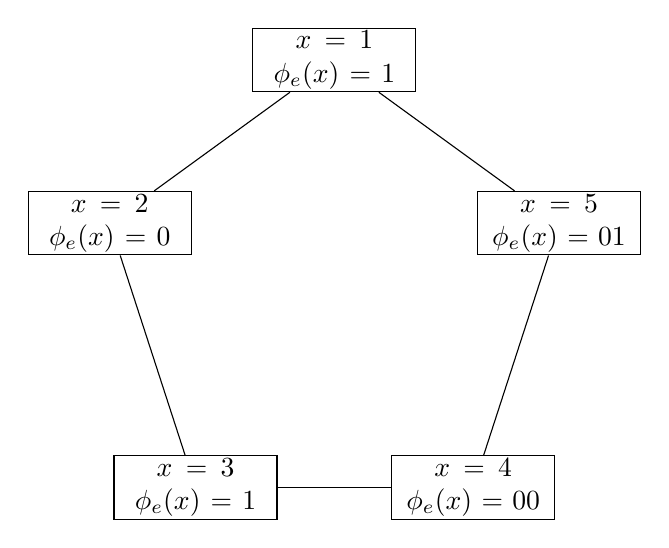
\begin{tikzpicture} 
[
  node distance=0.5cm,
  every node/.style={ draw, minimum size=4mm, inner sep=1pt, font = \normalsize, text width = 2 cm, align = center},
  every edge/.style={draw, -} 
]

\node[draw=black] (1) at (0,3) {$x=1$ \\ $\phi_e(x) = 1$};
\node[draw=black] (2) at (-2.8531,0.9271) {$x=2$ \\ $\phi_e(x) = 0$};
\node[draw=black] (3) at (-1.7634,-2.4271) {$x=3$ \\ $\phi_e(x) = 1$};
\node[draw=black] (4) at (1.7634,-2.4271) {$x=4$ \\ $\phi_e(x) = 00$}; 
\node[draw=black] (5) at (2.8531,0.9271) {$x=5$ \\ $\phi_e(x) = 01$}; 

\draw  (1) edge (2);
\draw  (3) edge (2);
\draw  (3) edge (4);
\draw  (4) edge (5);
\draw  (5) edge (1);
\end{tikzpicture}
    \caption{Variable length code employed by Alice.}
    \label{fig:c5_vlc_encoding}
\end{figure}
Since adjacent vertices are not prefixes of each other, this is an encoding that meets the criterion of \cite{AlonO_96} and is a non-singular code. 
In the single-instance case, this is a valid code. However, if we consider extension of the code, the encoding causes error. Suppose Bob observes $[2 ~ 4]$. Consider the following two cases. %\aditya{can be shortened}\meng{shortened}
\begin{enumerate}
    \item Suppose that Alice observes $[2~ 5]$. She uses the extension of $\phi_e$ and sends $(\phi_e(2),\phi_e(5) ) = 001$. The function value should be $[\tilde g(2,2)~\tilde g(5,4)]=[1~0]$. %\aditya{Should be tilde-g}\meng{Done}
    \item Suppose that Alice observes $[4~ 1]$. She uses the extension of $\phi_e$ and sends $(\phi_e(4),\phi_e(1) ) = 001$. The function value should be $[\tilde g(4,2)~\tilde g(1,4)]=[1~1]$. %\aditya{Should be tilde-g}\meng{Done}
\end{enumerate}
We observe that the function evaluations in the cases above are different, but the messages sent to Bob are all the same, i.e. "001". Therefore, Bob cannot unambiguously distinguish between the cases.%, and cannot have zero-error decoding. 
\end{example}

\begin{example}  \label{example:C5_VLC_f} Consider the computation of the function $\tilde f$ ({\it cf.} Table \ref{table:simple_eg1}) where the probability distribution is given in Table \ref{table:simple_eg1_pxy}. Suppose  Alice still uses the same encoding as the previous example, i.e., the encoding in Fig. \ref{fig:c5_vlc_encoding}. Compared to Example \ref{example:C5_VLC}, the same encoding meets the prefix-free code criterion ({\it cf.} Section \ref{subsubsec:VLC_setting}) because  $(X,Y)$ is taking value in a smaller set. Therefore, this code can be extended. 

This encoding is a $4$-coloring of the graph. However, it is not a regular prefix-free encoding of the colors. For example, $\phi_e(2)=0$ is a prefix of $\phi_e(4)=00$ and $\phi_e(5)=01$.  
\end{example}

The following results will be used to bound the optimal VLC rates. See  Appendix \ref{app:proof_lemma_graph_entropy} for the proof of Lemma \ref{lemma:prefix_free_OR_prod}, Lemma \ref{lemma:ont_shot_entropy_OR_prod} and Lemma \ref{lemma:graph_entropy} \ref{lemma:chromatic_entropy_chi_upper_bound} and \ref{lemma:korner_entropy_chi_f_upper_bound}.% \aditya{statement of lemma needs to change}\meng{Done, proof is also modified}
\begin{lemma}\label{lemma:prefix_free_OR_prod}
%Suppose all $x\ne x'$ and $(x,x')\notin E(G)$ are due to C2. 
For a $f$-confusion graph $G$, suppose that all $(x,x')\notin E(G)$ are due to C2.  Let $\phi_e$ be an arbitrary prefix-free encoding function for $G^{(m)}$, and  $\text{Im}(\phi_e)$ be the image set of encoding $\phi_e$. If $(\zeta_1,\zeta_2)$ is such that  $\zeta_1\ne \zeta_2$ and $\zeta_1,\zeta_2\in \text{Im}(\phi_e)$,  then $\zeta_1$ is not a prefix of $\zeta_2$ and vice versa. %\aditya{rewrote, CHECK}\meng{Done}
\end{lemma} 
%\aditya{maybe give an example here}\meng{The new way I state this lemma should be clear enough.}
\begin{lemma}\label{lemma:ont_shot_entropy_OR_prod}
Let the alphabet be $D$-ary. For a $f$-confusion graph $G$, suppose that all $(x,x')\notin E(G)$ are due to C2. Then $R_{VLC}^{(1)} \ge H_{\chi,D}(G,X)$ where $X$ has distribution function $p_X(\cdot)$.%, i.e. the marginal distribution from $p_{XY}(x,y)$.
    %Let the alphabet be $D$-ary. If all $x\ne x'$ and $(x,x')\notin E(G)$ are due to C2, then $R_{VLC}^1 \ge H_{\chi,D}(G,X)$ where $X$ has distribution function $p_X(x)$, i.e. the marginal distribution from $p_{XY}(x,y)$.
\end{lemma}%\meng{lemma is re-stated for new definition, proof is updated to d-ary}

%\aditya{General comment - need to be clear on what the entropy base is.}\meng{Done}
%revised
\begin{definition}{\it $D$-ary K\"orner's graph entropy.} 
\label{def:korner_entropy}
Let $\Gamma(G)$ denote the set of all independent sets of $G$. Let $X$ be distributed over the vertices of $G$. Then, the $D$-ary K\"orner's graph entropy $H_{\kappa}(G,X)$ is 
\begin{align*}
    H_{\kappa,D}(G,X)=\min_{X\in Z\in\Gamma(G)}I_D(X;Z)
\end{align*}
where   the minimization is taken over all conditional distributions $p_{Z|X}(z|x)$ with $Z$ taking value in $\Gamma(G)$. The constraint "$X\in Z\in\Gamma(G)$"  means that  the random variable $X$ belongs to the random independent set $Z$ with probability one. If $D=2$, then we just denote it $H_{\kappa}(G,X)$.
\end{definition} 
\begin{lemma} \label{lemma:graph_entropy}
\begin{enumerate}[label=(\alph*)]
    \item $\lim_{m\to \infty}\frac{1}{m}H_{\chi,D}(G^{\lor m},\bfX) = H_{\kappa,D}(G,X)$ (Theorem 5 of \cite{AlonO_96}). \label{lemma:chromatic_entropy_OR_prod_limit}
    \item If $\bfX$ is uniformly distributed over   $V(G^{(m)})$, then $H_{\chi,D}(G^{(m)},\bfX) \ge \log_D \left(\frac{|V(G^{(m)})|}{\alpha(G^{(m)})}\right)$ (Lemma 10 of \cite{AlonO_96}).\label{lemma:chromatic_entropy_ind_set_lower_bound}
    \item  $H_{\chi,D}(G^{(m)},\bfX) \le \log_D \chi(G^{(m)}).$   \label{lemma:chromatic_entropy_chi_upper_bound}
    \item  $H_{\kappa,D}(G^{(m)},\bfX) \le H_{\chi,D}(G^{(m)},\bfX)$ (Section V-B of \cite{AlonO_96}). \label{lemma:korner_vs_chromatic_entropy}
    \item $H_{\kappa,D}(G^{(m)},\bfX) \le \log_D \chi_f(G^{(m)})$. \label{lemma:korner_entropy_chi_f_upper_bound}
\end{enumerate}
\end{lemma} 
%\meng{Proof of part 3) 5) of above lemma is adapted to D-ary.}
For  Lemma \ref{lemma:graph_entropy} \ref{lemma:chromatic_entropy_OR_prod_limit}, \ref{lemma:chromatic_entropy_ind_set_lower_bound}, \ref{lemma:korner_vs_chromatic_entropy}, \cite{AlonO_96} proved the binary case, i.e., $D=2$. The binary case immediately implies the $D$-ary case because $H(X) = \frac{\ln D}{\ln 2}H_D(X),I(X;Y) = \frac{\ln D}{\ln 2}I_D(X;Y).$

\section{Analyzing the behavior of quantum advantage with VLC}\label{sec:analysis_bahavior_quantum_advantage_vlc} 

%\aditya{needs some rewording to smoothen the language} \meng{Done some attempt.}
In this section, we compare variable length prefix-free codes with quantum codes. The alphabet is binary throughout. %We use $H(X),I(X,Y),H_{\chi}(G,X),H_{\kappa}(G,X)$ for entropy, mutual information, chromatic entropy and K\"orner's graph entropy respectively. 
The comparison is for both single-instance and multiple instances. In the single-instance setting, we compare $\log_2\xi(\overline{G})$ and $R^{(1)}_{VLC}$ ({\it cf.} Definition \ref{def:VLC_rate}). In the multiple-instance setting, we compare $R_{\text{quantum}}$ ({\it cf.} Theorem \ref{thm:theorem4}) and $R_{VLC}$ ({\it cf.} Definition \ref{def:VLC_rate}).  There are three possibilities.  The rate of VLC can be strictly less than, or strictly larger than, or equal to  the quantum rate. We call them VLC advantage, quantum advantage and equivalent rates respectively. We will revisit examples that are used in the quantum vs. FLC comparison where $p_X(\cdot)$ is uniform. While some of them have a similar result as the FLC case, there are  examples leading to different results.

\subsection{VLC advantage   in both single-instance and multiple-instance  setting\label{sec:VLC_k3}}
 
%\aditya{Carefully think about examples and see if anything needs to change}
As pointed out in Remark \ref{remark:VLC_depends_on_p_X}, the VLC rate also depends on $p_{\bfX}(\cdot)$. On the other hand, the quantum rate and the FLC rate only depend upon $G^{(m)}$. Thus, the rate of the VLC rate can be very small for a ``favorable'' marginal distribution $p_{\bfX}(\cdot)$. We demonstrate this by means of an example below.


%As a consequence,    $p_{XY}(x,y)$ can be chosen such that   VLC rate is very low. One strategy  is to let the probability $p_{X}(x)$ concentrate on a small subset of $\calX$. Here is the example. 

Let $\epsilon>0$ be sufficiently small, $\calX=\{x_0,x_1,x_2\}$, and $\calY=\{y_0\}$ and $f(x,y) = x$.  We set 
\begin{align*}
 p_{XY}(x,y) =&\begin{cases}
     1-\epsilon,\text{ if }(x,y)=(x_0,y_0),\\
     \epsilon/ 2 \text{ if }(x,y) = (x_1,y_0),\\
     \epsilon/2  \text{ if }(x,y) = (x_2,y_0),
 \end{cases}%\text{ and }  f(x,y) = x. 
\end{align*} 
The single-instance $f$-confusion graph is $K_3$, and the multiple-instance $f$-confusion graph is $K_3^{\boxtimes m}=K_3^{\lor m}$. Therefore, the single-instance and multiple-instance quantum rate is $\log_2 3 = 1.58$.

In comparison, in the single-instance setting, Alice can use the following encoding:
\begin{align*}
    x_0\mapsto 0, x_1\mapsto 10, x_2\mapsto 11. 
\end{align*}
The expected code length is $(1-\epsilon)\cdot 1 + \frac{\epsilon}{2}\cdot 2+ \frac{\epsilon}{2}\cdot 2 = 1+\epsilon < \log_2 3$ for sufficiently small $\epsilon$. In the multiple-instance case, suppose Alice sends $\bfx$ using the Huffman code, then the asymptotic rate is $H(1-\epsilon,\epsilon/2,\epsilon/2) = H_2(\epsilon) + \epsilon$. This can be made arbitrarily close to $0$ by letting $\epsilon \to 0$.

\subsection{VLC advantage in single-instance setting, but equivalent rate  in multiple-instance setting.\label{sec:VLC_C5_AND}}
Consider function $\tilde f$. Let $p_{XY}(\cdot,\cdot)$  be shown in Table \ref{table:simple_eg1_pxy}. Recall that the $f$-confusion graph is $C_5^{\boxtimes m}$. From Proposition \ref{prop:C5_AND_rates}, we have $\log_2\xi(\overline{C_5}) =\log_23\approx 1.585$, $R_{\text{quantum}}(\tilde f)  =\frac{1}{2}\log_2 5$. The following proposition proved in Appendix \ref{app:proof_VLC_rate_c5} shows $\tilde f$ is the example we need.
\begin{proposition}\label{prop:VLC_rate_c5_AND}
\begin{enumerate}
    \item $R^{(1)}_{VLC}(\tilde f) = 1.4$.
    \item $R_{VLC}(\tilde f)=\frac{1}{2}\log_2 5$.
\end{enumerate}
\end{proposition}


%\aditya{Have to explain that we have to resort to numerical calculation of Korner entropy based on Blahut-Arimoto algorithm}

\subsection{Quantum advantage in single-instance setting, but equivalent rate  in multiple-instance setting.\label{sec:VLC_C5_OR}}
Consider function $\tilde g$. Let $p_{XY}(\cdot,\cdot)$  be shown in Table \ref{table:simple_eg2_pxy}. Then, $f$-confusion graph is $C_5^{\lor m}$. From Proposition \ref{prop:C5_AND_rates}, we have $\log_2\xi(\overline{C_5}) =\log_23\approx 1.585$,   $R_{\text{quantum}}(\tilde g) =  \log_2 \frac{5}{2}$. The following proposition proved in Appendix \ref{app:proof_VLC_rate_c5} shows  $\tilde g$ is the example we need.
\begin{proposition}\label{prop:VLC_rate_c5_OR}
\begin{enumerate}
    \item $ R^{(1)}_{VLC}(\tilde g) = 1.6$.
    \item  $R_{VLC}(\tilde g) =  \log_2 \frac{5}{2}$.
\end{enumerate}
\end{proposition}
\begin{remark}
   For Sections \ref{sec:VLC_C5_AND} and \ref{sec:VLC_C5_OR}, if we allow ternary ($D=3$) alphabet for classical communication and qutrits for quantum communication, then they would have same single-instance rate, which equals 1. This is because the rate is at least one. For quantum communication, $\xi(C_5) =3$ implies only one qutrit is needed. For VLC, the $3$-coloring of $C_5$ already induces an encoding of expected length 1.
   %
   %Why? We note the (expected) number of trit or qutried needed is at least 1.  For quantum communication, $\xi(C_5) =3$ implies only one qutrit is needed. For VLC,    the $3$-coloring of $C_5$ already induces an encoding of expected length 1.
\end{remark} 
\subsection{Quantum advantage both in single-instance and in multiple-instance setting.\label{sec:VLC_quantum_in_single_and_multi_instance}}

In this section, we use the characterization of the asymptotic VLC rate corresponding to $G^{\lor m}$ as the {K\"orner} entropy ({\it cf.} Definition \ref{def:korner_entropy}). A numerical computation of  {K\"orner} graph entropy requires optimizing over the class of independent sets in $G$. For smaller graphs, such an enumeration is feasible. Moreover, the work of \cite{HarangiNB24} provides a Blahut-Arimoto-like algorithm for computing  K\"orner's graph entropy. We use their method in our calculations.

\subsubsection{Example associated with OR product.}  \label{sec:VLC_G13}
By Theorem \ref{thm:construct_function_based_on_G} and Remark \ref{remark:free_to_choose_p_x}, there exists a function and a joint distribution such that its $m$-instance $f$-confusion graph is $G_{13}^{\lor m}$ ({\it cf.} \ref{subsubsec:G13}) and $p_X(\cdot)$ is uniform over $\calX$.  From Proposition \ref{prop:G_13_quantum_rate}, we have that $  R_{\text{quantum}}(G_{13}) = \log_2\xi(G_{13}) = \log_2 3=1.585$. 

 By Theorem \ref{thm:VLC_optimal_rate} and  Lemma \ref{lemma:graph_entropy}     \ref{lemma:chromatic_entropy_OR_prod_limit}, $R_{VLC} = \lim_m\frac{1}{m} H_{\chi,D}(G_{13}^{\lor m},\bfX) = H_{\kappa}(G_{13},X)$. By Lemma \ref{lemma:ont_shot_entropy_OR_prod} and  Lemma \ref{lemma:graph_entropy}  \ref{lemma:korner_vs_chromatic_entropy}, $R_{VLC}^{(1)}(G_{13},X)\ge H_{\chi}(G_{13},X)\ge H_{\kappa}(G_{13},X)$. 

%We numerically calculated in \cite{meng2024github}  by using  

We used the method provided  in \cite{HarangiNB24} and obtained $H_{\kappa}(G_{13},X) \approx 1.646$ (code available at \cite{meng2024github}). %\aditya{Ruoyu include link} \meng{Done} 
This implies there is a   quantum advantage in both multiple-instance and single-instance setting. 

\subsubsection{Example associated with strong product.} \label{sec:VLC_Hn}
Consider a function and a joint distribution such that its single-instance $f$-confusion graph $H_n$ ({\it cf.} \ref{subsubsec:Hn}) and $p_X(\cdot)$ is uniform over $\calX$.  By Theorem \ref{thm:construct_function_based_on_G} and Remark \ref{remark:free_to_choose_p_x}, there exists such a function and a joint distribution.

%\meng{Just in case you ask. I also checked Lemma no. from the paper of Lemma below, and it is correct.}
\begin{proposition}[Lemma 5.5 of \cite{BrietBL_15}]\label{prop:upper_bound_alpha_H_n}
    \begin{align*}
       \alpha((H_n^{\lor m})^{\frac{1}{m}} \le \alpha((H_n^{ ( m)})^{\frac{1}{m}}\le \alpha((H_n^{\boxtimes m})^{\frac{1}{m}} < 2^{0.846n}\text{ for }m\ge 1.
    \end{align*}
\end{proposition}
Lemma 1 part \ref{lemma:chromatic_entropy_ind_set_lower_bound} and the above Proposition gives
\begin{align*}
\frac{1}{m}H_{\chi}(G^{(m)},\bfX)\ge \frac{1}{m} \log \frac{|V(G^{(m)})|}{\alpha(G^{(m)})} \ge \log \frac{2^{n}}{2^{0.864n}} = {0.154 n}.
\end{align*}
%\meng{I found that the orthogonal representation I used is already in the Briet's paper, so I revised the next proposition.} 
We already showed in Section \ref{subsubsec:Hn} that  
\begin{align*} n+1  \ge \xi(\overline{H_n^{\lor m}})^{\frac{1}{m}}\ge\xi(\overline{H_n^{(m)}})^{\frac{1}{m}} \ge \xi(\overline{H_n^{\boxtimes m}})^{\frac{1}{m}}\text{ for }m\ge 1.
\end{align*}
Then we have
\begin{align*}
    R_{VLC} \ge 0.154n > \log (n +1)\ge  \frac{\log_2\xi(\overline{H_n^{\boxtimes }})}{m}\ge R_{\text{quantum}}.
\end{align*}
This gives the following conclusion. If the marginal distribution $p_X(\cdot)$ is uniform, then both $H^{\lor m},H^{\boxtimes m}$ are $f$-confusion graphs where the quantum rate is exponentially smaller than the VLC rate.% exponential quantum advantage.

\subsection{Quantum advantage   in single-instance setting, but VLC advantage in multiple-instance setting.\label{sec:VLC_line_graph}}



Consider a function and a joint distribution such that its $m$-instance $f$-confusion graph $\frL(G_{13})^{\lor m}$ ({\it cf.} \ref{sec:line_graph_eg}) and $p_X(\cdot)$ is uniform over $\calX$. From Section \ref{sec:line_graph_eg}, we have that $R_{\text{quantum}}(\frL(G_{13}))=\log_2\xi(\frL(G_{13}))=\log_2 3.$ 

Since the $f$-confusion graph is the OR product, all $x\ne x'$ and $(x,x')\notin E(G)$ are due to condition $C2$ by Theorem \ref{thm:theorem4} \ref{thm:theorem4_part_b}. Then,  $R_{VLC}^{(1)}(\frL(G_{13}),X)\ge H_{\chi}(\frL(G_{13}),X)$ by Lemma \ref{lemma:ont_shot_entropy_OR_prod}. We obtained a lower bound on $H_{\chi}(\frL(G_{13}),X)$ by numerical calculation (code available at \cite{meng2024github}), which is described as follows.  

We found $\alpha(\frL(G_{13}))=18$  by numerical calculation. Since every independent set of a graph is a clique of its complement graph, $\alpha(\frL(G_{13}))= \omega(\overline{\frL(G_{13})})$. We used Bron-Kerbosch algorithm \cite{BronKerbosch73} on $\overline{\frL(G_{13})}$ to enumerate all maximal clique sets and calculated $\omega(\overline{\frL(G_{13})})$. 

 Let $c$ be the coloring of  $\frL(G_{13})$ that achieves $H_{\chi}(G,X)$, and $C_1,C_2,\dots, C_k$ each color class (vertex set of same color). Recall that Claim \ref{claim:chi(L(G13)=4} states $\chi(\frL(G_{13})) = 4$. Then, the number of colors  $k\ge \chi(\frL(G_{13}))=4$.  Define  $\beta_i:=|C_i|,i\in k$. Since $p_X(\cdot)$ is uniform, we have 
\begin{align*}
  H_{\chi}(\frL(G_{13}),X)= \sum_{i=1}^k - \frac{|C_i|}{|V(\frL(G_{13}))|} \log_2 \Big  (\frac{|C_i|}{|V(\frL(G_{13}))|}\Big  )= \sum_{i=1}^k - \frac{\beta_i}{|V(\frL(G_{13}))|} \log_2 \Big (\frac{\beta_i}{|V(\frL(G_{13}))|}\Big ).
\end{align*} 
Since each color class is an independent set, $\beta_i\le \alpha(\frL(G_{13})) = 18$ for each $i$. The sum of size of all color classes must equal the number of vertices.  Therefore, we have
\begin{equation}\label{eq:line_graph_color}
        \sum_{i=1}^k\beta_i=|V(\frL(G_{13}))| = 48\text{ and }\beta_i\le 18, \forall i\in[k].
\end{equation}
Without loss of generality, we assume that $\beta_1\ge \beta_2 \ge \dots \ge \beta_k$. It turns out $(\beta_1, \beta_2 , \dots , \beta_k)$ can be viewed as an integer partition of 48 such that the number of parts $k$ is at least $\chi(\frL(G_{13})=4$  and each part  $\beta_i$  is at most $\alpha(\frL(G_{13})=18$. In particular, Sagemath has a built-in method to enumerate all such $(\beta_1, \beta_2 , \dots , \beta_k)$'s. Upon calculating the quantity 
\begin{align*}
    \sum_{i=1}^k - \frac{\beta_i}{|V(\frL(G_{13}))|} \log_2 \Big (\frac{\beta_i}{|V(\frL(G_{13}))|}\Big ),
\end{align*}
the minimum value obtained was $1.66$ (code available at \cite{meng2024github}). Therefore, we conclude that 
\begin{align*}
     H_{\chi}(\frL(G_{13}),X)\ge 1.66>\log_2 3.
\end{align*}
 By Theorem \ref{thm:VLC_optimal_rate} and  Lemma \ref{lemma:graph_entropy} \ref{lemma:chromatic_entropy_OR_prod_limit}, $R_{VLC} = \lim_m\frac{1}{m} H_{\chi,D}(\frL(G_{13})^{\lor m},\bfX) = H_{\kappa}(\frL(G_{13}),X)$. Using the method in \cite{HarangiNB24} we obtained $H_{\kappa}(\frL(G_{13}),X) = 1.45 < \log_2 3$ (code available at \cite{meng2024github}).
   
\section{Conclusions and Future Work}
\label{sec:conclusion}

In this work, we considered the problem of function computation with side information under the zero-error constraint. Alice and Bob have sources $X$ and $Y$ respectively with joint p.m.f. $p_{XY}(X,Y)$ and Bob wants to compute $f(X,Y)$. In all three settings (FLC, VLC and quantum), the $f$-confusion graph $G$ and its $m$-instance version $G^{(m)}$ plays a key role in the analysis of the optimal rate. We provided a characterization of necessary and sufficient conditions on the function $f(\cdot, \cdot)$ and joint p.m.f. $p_{XY}(\cdot,\cdot)$ such that $G^{(m)}$ equals  $G^{\boxtimes m}$ (strong product) or $G^{\lor m}$ (OR product). In general, $G^{(m)}$ lies in between these two extremes. We compared quantum rate versus FLC rate and  quantum rate versus VLC rate, and presented several examples of $f$-confusion graphs that demonstrate the varied behavior of the quantum advantage, when considering the single-instance and asymptotic rates. 

%It would be interesting to examine whether there are $f$-confusion graphs where there is no quantum advantage in the single-instance rate, but there is a quantum advantage in the asymptotic rate in the quantum-FLC comparison.
%\meng{TODO: Conclusion needs to discuss VLC}
%----------------------------------------
%
%----------------------------------------
 
\newpage


  
\bibliographystyle{IEEEtran}
\bibliography{ref} 

\newpage
\thispagestyle{empty} % Makes the page style empty (no headers/footers)

% Insert a completely blank page
\mbox{}

% Force the compiler to create the blank page
\appendices





 \section{Proofs of proposition \ref{prop:chi}} \label{app:appendix_A}


\subsection{Proof of Proposition \ref{prop:chi} \ref{prop:de_morgan}}
\begin{proof}
We only need to show that $E\big (    \overline{G\boxtimes H} \big ) = E\big (    \overline{G}\lor \overline{H}  \big )$. Toward this end, note that
\begin{align*}
&\big( (v_1,u_1),(v_2,u_2) \big)\in E\big (    \overline{G\boxtimes H} \big )\\
\Leftrightarrow&\big( (v_1,u_1),(v_2,u_2)\big) \notin E\big (    G\boxtimes H  \big )\text{~and~}(v_1,u_1)\ne(v_2,u_2)\\
\Leftrightarrow&\big( v_1\ne v_2\text{ and }(v_1,v_2)  \notin E(G) \big )\text{ or } \\
&\big( u_1\ne u_2\text{ and }(u_1,u_2) \notin E(H) \big ) \\
\Leftrightarrow&\big( (v_1,u_1),(v_2,u_2) \big)\in E\big (    \overline{G}\lor \overline{H}  \big ).
\end{align*}
We conclude that $E\big (    \overline{G\boxtimes H} \big ) = E\big (    \overline{G}\lor \overline{H}  \big )$.
\end{proof}



%\subsection{Proof of Proposition \ref{prop:chi} \ref{prop:AND_prod_distrib}}
%\begin{proof}
%    \begin{align*}
%        V(G\boxtimes (H_1\cup H_2)) = &V(G)\times V(H_1\cup H_2)\\
%        = &V(G)\times V(H_1)\cup V(G)\times V(H_2) .
%    \end{align*}
%    Let  $u_1,u_2\in V(G), v_1, v_2\in V(H_1\cup H_2)$ be arbitrary. Case $u_1=u=u_2$ for some $u\in V(G)$:
%    \begin{align*}
%&       \big( (u,v_1),(u,v_2)\big)\in E(G\boxtimes (H_1\cup H_2))\\
%       \Leftrightarrow& (  v_1 ,v_2 )\in E( H_1\cup H_2 )\\
%        \Leftrightarrow&  ( v_1 ,v_2 )\in E( H_1)\text{ or }(v_1 ,v_2)\in E( H_2 )\\
%        \Leftrightarrow& \big( (u,v_1),(u,v_2)\big)\in E( G\boxtimes H_1)\\&\text{ or }\big((u,v_1),(u,v_2)\big)\in E( G\boxtimes H_2 ).
%    \end{align*}
%Case   $v_1=v=v_2$ for some $v\in V(H_1\cup H_2)$:
%    \begin{align*}
%&        \big((u_1,v),(u_2,v)\big)\in E(G\boxtimes (H_1\cup H_2))\\
%        \Leftrightarrow&  ( u_1 ,u_2 )\in E( G )\\ 
%        \Leftrightarrow& \big( (u_1,v),(u_2,v) \big)\in E( G\boxtimes H_1)\\&\text{ or }\big( (u_1,v),(u_2,v) \big)\in E( G\boxtimes H_2 ).
%    \end{align*}
%Case   $u_1\ne u_2, v_1\ne v_2$:
%    \begin{align*}
%&       \big( (u_1,v_1),(u_2,v_2)\big)\in E(G\boxtimes (H_1\cup H_2))\\
%        \Leftrightarrow& ( u_1 ,u_2 )\in E( G ) \text{ and }( v_1 ,v_2) \in E( H_1\cup H_2 )\\
%        \Leftrightarrow&  ( u_1 ,u_2 )\in E( G ) \\&\text{ and }\Big ( (v_1 ,v_2) \in E( H_1)\text{ or }(v_1 ,v_2)\in E( H_2 ) \Big )\\
%        \Leftrightarrow& \big( (u_1,v_1),(u_2,v_2) \big)\in E( G\boxtimes H_1)\\&\text{ or }\big( (u_1,v_1),(u_2,v_2) \big)\in E( G\boxtimes H_2 ).
%    \end{align*}
%It follows that $E(G\boxtimes (H_1\cup H_2)) =  E(G\boxtimes H_1)\cup E(G\boxtimes H_2) $
%\end{proof}




\subsection{Proof of Proposition \ref{prop:chi} \ref{prop:alpha_AND_OR_product}}
\begin{proof} 




    Let $S_1$ and $S_2$ be independent sets in $G$ and $H$ respectively. Then, $S_1\times S_2$ is independent in $G\lor H$. Thus, $\alpha(G\lor H) \ge \alpha(G)\alpha(H)$. Now we show the other inequality. Let $S$ be a maximum independent set in $G\lor H$. Define 
    \begin{align*}
        &S_g := \{g\in V(G): \exists h\in V(H), (g,h) \in S\},
        \\  &S_h := \{h\in V(h): \exists g\in V(G), (g,h) \in S\}
    \end{align*}
    The role of $S_g,S_h$ is interchangeable, so it suffices to show $S_g$ is independent in $G$. Let distinct $g_1,g_2\in S_g$. Then there exist $h_1,h_2$ such that   $(g_1,h_1),(g_2,h_2)\in S$. Since $S$ is independent in $G\lor H$, $(g_1,h_1),(g_2,h_2)\notin E(G\lor H)$ and thus $(g_1,g_2)\notin E(G)$. It follows that $S_g$ is  independent.  Therefore, $\alpha(G\lor H) \le \alpha(G)\alpha(H)$ holds.
    
For $\alpha(G)\alpha(H)\le \alpha(G\boxtimes H),$ we note that if   $S_1$ and $S_2$ are independent in $G$ and $H$ respectively, then $S_1\times S_2$ is independent in $G\boxtimes H$. Then, $\alpha(G\boxtimes H) \ge \alpha(G) \alpha(H)$ holds.
\end{proof}



 



\subsection{Proof of Proposition \ref{prop:chi} \ref{prop:chi_product}}
\begin{proof}
$\chi(G\boxtimes H)\le\chi(G\lor H)$ holds because $G\boxtimes H\subseteq G\lor H$.

If $c:V(G)\mapsto [\chi(G)]$ and $d:V(H)\mapsto [\chi(H)]$ are proper colorings  of $G$ and $H$ respectively, then 
\begin{align*}c\times d:V(G)\times V(H)&\mapsto [\chi(G)]\times [\chi(H)],\\
(u,v) &\mapsto (c(u),d(v))
\end{align*}  is a proper coloring of $G\lor H$. Therefore, $\chi(G \lor H) \le \chi(G)\chi(H).$
\end{proof}




 

\section{Proof of Proposition \ref{prop:AND_power_m-instance_graph_OR_power}}
 


 \label{app:pf_prop5}





\begin{proof}Since the vertex sets of $G^{\boxtimes m}, G^{(m)}, G^{\lor m}$ are the same, namely $\calX^m$, it suffices to show  $E(G^{\boxtimes m})\subseteq E(G^{(m)})\subseteq E(G^{\lor m})$. 

Let $(\bfx,\bfx')\in E(G^{\boxtimes m})$ and $\bfx\ne \bfx'$. There exists $  i$ such that  $x_{  i}\ne x_{  i}'$ because  
  $\bfx\ne \bfx'$. For such $i$ indices, $(x_i,x_i')\in E(G)$, so there exists $y_i$ such that  $p_{XY}(x_i,y_i)p_{XY}(x_i',y_i)>0$ and $f(x_i,y_i)\ne f(x_i',y_i)$.  For the remaining $i$ indices such that  $x_i= x_i'$, there exists $y_i$ such that  $p_{XY}(x_i,y_i)>0$ by Assumption \ref{assume:irreducible}. Let $\bfy = \{y_i\}_{y=1}^m$. Then we have
\begin{align*}
p_{\bfX\bfY}(\bfx ,\bfy)p_{\bfX\bfY}(\bfx' ,\bfy) > 0\text{ and } f^{(m)}(\bfx ,\bfy) \neq f^{(m)}(\bfx' ,\bfy).
\end{align*}
Therefore, $(\bfx,\bfx')\in E(G^{(m)})$. It implies $E(G^{\boxtimes m})\subseteq E(G^{(m)})$ as  $(\bfx,\bfx')\in E(G^{(m)})$ is arbitrary.



Let $(\bfx,\bfx')\in E(G^{(m)})$ be arbitrary. Then, there exists $\bfy$ such that $ p_{\bfX\bfY}(\bfx ,\bfy)p_{\bfX\bfY}(\bfx' ,\bfy) > 0$ and   $f^{(m)}(\bfx ,\bfy) \neq f^{(m)}(\bfx' ,\bfy)$. It implies that  there exists $j \in [m]$ such that $p_{XY}(x_{j},y_j) p_{XY}(x_{j}', y_j) > 0$ and $f(x_{j},y_j) \neq f(x_{j}',y_j)$, i.e. $(x_j,x_j')\in E(G).$ This implies $(\bfx,\bfx')\in E(G^{\lor m})$. Thus, $E(G^{(m)}) \subseteq  E(G^{\lor m})$  as $(\bfx,\bfx')\in E(G^{\lor m})$ are   arbitrary.
\end{proof}




%\begin{proof}
%We show $G^{(m)}\boxtimes G \subseteq G^{(m+1)} \subseteq G^{(m)}\lor G$ first.  Recall that $G^{(m+1)}$ has vertex set $\{\bfx\in \calX^{m+1} \}$ and vertices $\bfx_1$ and $\bfx_2$ are connected if there exists $\bfy$ such that $\Pi_{i=1}^{m+1} p_{XY}(x_{1i},y_i) p_{XY}(x_{2i}, y_i) > 0$ and there exists $j \in [m+1]$ such that $f(x_{1j},y_j) \neq f(x_{2j},y_j)$.

%Since the vertex sets of $G^{(m)}\boxtimes G, G^{(m+1)}, G^{(m)}\lor G$ are the same, that is $\calX^{m+1}$, it suffices to show  $E(G^{\boxtimes m})\subseteq E(G^{(m)})\subseteq E(G^{\lor m})$. For $\bfx=\{x_i\}_{i=1}^{m+1}\in \calX^{m+1}$ and $\bfy=\{y_i\}_{i=1}^{m+1}\in \calY^{m+1}$, denote $\overline{\bfx}:=\{x_i\}_{i=1}^m$ and $\overline{\bfy}:=\{y_i\}_{i=1}^m$  respectively. 

% Let $(\bfx,\bfx')\in E(G^{(m)}\boxtimes G)$. In the case $(\overline{\bfx},\overline{\bfx}')\in E(G^{(m)})$, there exists $\hat \bfy = \{y_i\}_{i=1}^m\in \calY^m$ be such that  $p_{\bfX\bfY}(\overline{\bfx},\hat \bfy)p_{\bfX\bfY}(\overline{\bfx}',\hat \bfy)>0$ and $f^{(m)}(\overline{\bfx},\hat \bfy)\ne f^{(m)}(\overline{\bfx}',\hat\bfy)$. Both $x_{m+1}=x_{m+1}'$ and $(x_{m+1},x_{m+1}')\in E(G)$ implies existence of $y_{m+1}\in \calY$ such that  $p_{XY}(x_m,y_m)p_{XY}(x_m',y_m)>0$.  In the case $(\overline{\bfx},\overline{\bfx}')\notin E(G^{(m)})$,  we must have $\overline{\bfx}=\overline{\bfx}'$ and $(x_{m+1},x_{m+1}')\in E(G)$. Then there exists $\hat \bfy\in\calY^{m}$ such that   $p_{\bfX\bfY}(\overline{\bfx},\hat \bfy)p_{\bfX\bfY}(\overline{\bfx}',\hat \bfy)>0$. And there exists $y_{m+1}\in\calY$  such that  $p_{XY}(x_{m+1},y_{m+1})p_{XY}(x_{m+1}',y_{m+1})>0$ and $f (x_{m+1},y_{m+1})\ne f (x_{m+1}',y_{m+1})$. 
 
% In both cases, let $\bfy = \{y_i\}_{i=1}^{m+1}$. We have $p_{\bfX\bfY}( {\bfx},  \bfy)p_{\bfX\bfY}( {\bfx}',  \bfy)>0$ and $f^{(m+1)}( {\bfx},  \bfy)\ne f^{(m+1)}( {\bfx}', \bfy)$, which implies $(\bfx,\bfx')\in E(G^{(m+1)})$. Therefore, we have  $E(G^{(m)}\boxtimes G)\subseteq E(G^{(m+1)})$.
 
  

% Now let $(\bfx,\bfx')\in E(G^{(m+1)})$. Then, there exists $\bfy$ such that $\Pi_{i=1}^{m+1} p_{XY}(x_{i},y_i) p_{XY}(x_{i}', y_i) > 0$ and there exists $j \in [m+1]$ such that $f(x_{j},y_j) \neq f(x_{j},y_j)$. In particular, we have $p_{XY}(x_{j},y_j) p_{XY}(x_{j}', y_j) > 0$ and $f(x_{j},y_j) \neq f(x_{j},y_j)$. If $j=m+1$, then $(x_{m+1},x_{m+1}')\in E(G)$. This implies  $(\bfx,\bfx')\in E(G^{(m)}\lor G)$.

%Otherwise, it implies  $\overline{y}$ is such that  $p_{\bfX\bfY}(\overline{\bfx},\overline{ \bfy})p_{\bfX\bfY}(\overline{\bfx}',\overline{ \bfy})>0$ and $f^{(m)}(\overline{\bfx},\overline{ \bfy})\ne f^{(m)}(\overline{\bfx}',\overline{\bfy})$, i.e. $(\overline{\bfx},\overline{\bfx}')\in E(G^{(m)})$. This implies  $(\bfx,\bfx')\in E(G^{(m)}\lor G)$. Therefore, $E(G^{(m+1)})\subseteq E(G^{(m)}\lor G)$.

% $G^{\boxtimes m} \subseteq G^{(m)} \subseteq G^{\lor m}$ follows from the induction on $m$ using  $G^{(m)}\boxtimes G \subseteq G^{(m+1)} \subseteq G^{(m)}\lor G$. Note the base case $m=1$ holds because $G^{\boxtimes 1} = G^{(1)} = G^{\lor 1}$.



%\end{proof}


 

 


 
 

 
 

 

 
\section{Proofs of proposition \ref{prop:xi}}\label{app:appendix_C}


\subsection{Proof of Proposition \ref{prop:xi} 
 \ref{prop:subgraph_xi}}
\begin{proof}
%    Let $\phi$ be an orthogonal representation of $G$. $V(G)=V(H)$ as $G\subseteq H$ Since $V(G)=V(H)$, every vertex in $V(H)$ is assigned a vector. Let $u,v\in V(H)$ be non-adjacent in $H$. Since $G\subseteq H$, $u,v$ is also non-adjacent in $G$. Thus $\phi(u)\perp\phi(v)$.  Therefore, $\phi$ is also an orthogonal representation of $H$. This implies $\xi(H)\le \xi(G).$
Recall that we use $G\subseteq H$ to denote that $G$ is a spanning subgraph of $H$, i.e. $V(G) = V(H)$ and $E(G)\subseteq E(H)$. Therefore, every orthogonal representation of $G$ is an orthogonal representation of $H$.
\end{proof}



\subsection{Proof of Proposition \ref{prop:xi}  \ref{prop:xi_product}}
\begin{proof}
$\xi(G\lor H)\le \xi(G\boxtimes H)$ holds because of 
Proposition \ref{prop:xi} \ref{prop:subgraph_xi} and the fact that $G\boxtimes H\subseteq G\lor H$. 

Now we show that $\xi(G\boxtimes H)\le \xi(G)\xi(H).$ Suppose $\phi_G:V(G)\mapsto \bbC^{m_1},\phi_H:V(H)\mapsto \bbC^{m_2}$ are   orthogonal representations of $G,H$ respectively. We claim $$
\phi_G\times\phi_H:V(G)\times V(H) \mapsto \bbR^{m_1m_2}, (g,h)\mapsto \phi_G(g) \otimes \phi_H(h)
$$
where $\otimes$ denotes tensor product, is an orthogonal representation of $G\boxtimes H$. 

Indeed, let $(u_1,v_1),(u_2,v_2)$ be distinct and non-adjacent in $G\boxtimes H$. W.l.o.g., we assume $(u_1,u_2)\notin E(G)$ and $u_1\ne u_2$. Thus $\phi_G(u_1)\perp\phi_G(u_2)$. It follows that $\phi_G\times\phi_H(u_1,v_1)=\phi_G(u_1)\otimes\phi_H(v_1) \perp \phi_G(u_2)\otimes\phi_H(v_2)= \phi_G\times\phi_H(u_2,v_2)$.
\end{proof}


\subsection{Proof of Proposition \ref{prop:xi} \ref{prop:xi_chi_compare}}
\begin{proof}
Let $c:V(G)\mapsto[k]$ be a proper coloring of $\overline{G}$ and $e_i$ be the $i$-th elementary vector in $\bbC^{k}$ for $i\in[k]$. Then $c$ induces the following $k$-dimensional orthogonal representation of $G$.
$$
\phi:V(G)\mapsto \bbC^{k}, \phi(v)\mapsto e_i\text{ iff }c(v) = i.
$$
\end{proof}
 
\section{Proof of $\vartheta(G)\vartheta(H)=\vartheta(G\lor H)$}\label{app:vartheta_multiplicity}

From Theorem 7 of \cite{lovasz1979shannon}, we have that $\vartheta(G\boxtimes H) = \vartheta(G)\vartheta(H)$. Since $G\boxtimes H\subseteq G\lor H$, we have $\vartheta(G\lor H)\le \vartheta(G\boxtimes H) =\vartheta(G)\vartheta(H)$ by Lemma \ref{lemma:lovasz} \ref{prop:lovasz_number_subgraph}. Therefore, it suffices to show
\begin{align*}
    \vartheta(G)\vartheta(H)\le \vartheta(G\lor H).
\end{align*} 
We will use the following equivalent definition of $\vartheta(G)$.
\begin{theorem}[from \cite{lovasz1979shannon}]
    Let $G$ be a graph on vertices $[n]$. Let $\phi$ range over all orthogonal representation over $\overline{G}$ be s.t. $\phi(i)$ is a real vector for all $i\in V(G)$ and $d$ range over all real unit-norm vectors. Then 
    \begin{equation}\label{eqn:lovasz_number_thm5}
        \vartheta(G) = \max_{\phi,d}\sum_{i=1}^n(d^T\phi(i))^2
    \end{equation}
\end{theorem}
The proof  is mostly the same as the one in Theorem 7 of \cite{lovasz1979shannon}. We include it for completeness.
\begin{proof}[Proof of $ \vartheta(G)\vartheta(H)\le \vartheta(G\lor H)$]
Let $\phi$ and $c$ be an orthogonal representation of $G$ and a vector in  (\ref{eqn:lovasz_number_thm5}) that achieves $\vartheta(G)$, and $\psi$ and $d$ be an orthogonal representation of $H$ and a vector in   (\ref{eqn:lovasz_number_thm5})   that achieves $\vartheta(H)$. We have that $\phi \times\psi(i,j):= \phi(i) \otimes \psi(j)$
is an orthogonal representation of $\overline{G}\boxtimes \overline{H}$ by the same reason used in Proposition \ref{prop:xi} \ref{prop:xi_product}. Since $G\lor H =\overline{\overline{G}\boxtimes\overline{H}}$, we have
\begin{align*}
    \vartheta(G\lor H)  \ge &\sum_{i=1}^{|V(G)|}\sum_{j=1}^{|V(H)|} \Big ( (d\otimes c)^T (u_i \otimes v_j) \Big )^2\\
        = &\sum_{i=1}^{|V(G)|} \sum_{j=1}^{|V(H)|}(d^Tu_i)^2(c^Tv_j)^2\\
        =&\sum_{i=1}^{|V(G)|}  (d^Tu_i)^2\sum_{j=1}^{|V(H)|}(c^Tv_j)^2 = \vartheta(G)\vartheta(H)
\end{align*}
\end{proof}

 
%revised
\section{Proof of Lemma \ref{lemma_single_letter}}\label{app:proof_lemma_single_letter}
\begin{proof}
We have $\overline{G}^{\boxtimes m}= \overline{G^{\lor m}}\subseteq \overline{G^{(m)}}\subseteq \overline{G^{\boxtimes m}} =\overline{G}^{\lor m}$ due to Proposition \ref{prop:chi} \ref{prop:de_morgan} and Proposition \ref{prop:AND_power_m-instance_graph_OR_power}. Lemma \ref{lemma:lovasz} \ref{prop:lovasz_number_subgraph} and   \ref{lemma:lovasz_number_AND_product} implies that 
\begin{align*}
\vartheta(\overline{G})^m = \vartheta(\overline{G}^{\lor m}) \le  \vartheta(\overline {G^{(m)}})\le \vartheta(\overline{G}^{\boxtimes  m}) = \vartheta(\overline{G})^m.
\end{align*}
Lemma \ref{lemma:lovasz} \ref{lemma:lovasz_number_xi_compare} gives that $\vartheta(\overline {G^{(m)}})\le\xi(\overline {G^{(m)}})$.  Proposition \ref{prop:xi}     \ref{prop:xi_product} and \ref{prop:subgraph_xi} gives $\xi(\overline {G^{(m)}}) \le\xi(\overline{G}^{\boxtimes m})  \le  \xi(\overline {G})^{m}$. Combining everything, we have
\begin{equation}
    \vartheta(\overline{G})^m\le \xi(\overline {G^{(m)}}) \le  \xi(\overline {G})^{m}.\label{eq:sandwich_version2}    
\end{equation}
If $\vartheta(\overline{G})=\xi(\overline {G})$, then we have $\xi(\overline {G^{(m)}})^{\frac{1}{m}}=\xi(\overline {G})$ for all $m\ge 1$ by  (\ref{eq:sandwich_version2}). Therefore, \ref{lemma_single_letter_part_a} is proved. 

Lemma \ref{lemma:lovasz} \ref{lemma:lovasz_number_indep_compare} gives $\omega(G) = \alpha(\overline{G}) \le \vartheta(\overline{G})$. Proposition \ref{prop:xi} \ref{prop:xi_chi_compare} gives $\xi(\overline {G})\le \chi(G)$. Plugging them into   (\ref{eq:sandwich_version2}), we have
\begin{align*}
 \omega(G)^m   \le \vartheta(\overline{G})^m\le \xi(\overline {G^{(m)}}) \le  \xi(\overline {G})^{m}   \le \chi(G)^m.
\end{align*}
Similarly, for chromatic number, we have
\begin{align*}
 \omega(G)^m   \le \vartheta(\overline{G})^m\le \xi(\overline {G^{(m)}}) {\le}  \chi( {G^{(m)}})    \le \chi(G)^m.
\end{align*}
If $G$ is perfect, then $ \omega(G) = \chi(G)$. By the above inequalities, we have $\xi(\overline {G^{(m)}})^{\frac{1}{m}}=\xi(\overline {G})=\chi(G)=\chi( {G^{(m)}})^{\frac{1}{m}}$ for all $m\ge 1$.  
\end{proof}
 

% \section{Proofs of Theorem \ref{sandwich}} \label{app:pf_thm3}
% \begin{proof} 
% $\alpha(G^{\boxtimes m}) \le\vartheta(G ^{\boxtimes m})$ follows  from Lemma  \ref{lemma:lovasz} \ref{lemma:lovasz_number_indep_compare}.
% The equality  $\vartheta(G^{\lor m}) =\vartheta(G^{\boxtimes m}) = \vartheta(G)^m$ holds by Lemma \ref{lemma:lovasz} \ref{lemma:lovasz_number_AND_product}. 
% Since $G^{\boxtimes m}\subseteq G^{(m)} \subseteq G^{\lor m}$ by Proposition \ref{prop:AND_power_m-instance_graph_OR_power}, we have $$\vartheta(G)^m=\vartheta(G^{\boxtimes m}) \ge \vartheta(G^{(m)}) \ge \vartheta(G^{\lor m})= \vartheta(G)^m$$ by Lemma  \ref{lemma:lovasz} \ref{prop:lovasz_number_subgraph}. The inequality $\vartheta(G^{\lor m})\le \xi(G^{\lor m})$ follows from Lemma \ref{lemma:lovasz} \ref{lemma:lovasz_number_xi_compare}.  
% \end{proof}



%\section{Proofs of section VIII}



% \subsection{Proof  of Claim \ref{claim:claim1}}\label{app:pf_claim1}




% \begin{proof}
% By Proposition \ref{prop:xi} \ref{prop:subgraph_xi}, we have $\xi(\overline{C_5}) \le \chi(C_5) =3 $. Moreover, we know that $\overline{C_5}$ is isomorphic to $C_5$ and furthermore that $\vartheta(C_5) \le \xi(C_5)$. It is well known that $\vartheta(C_5) = \sqrt{5}$ \cite{lovasz1979shannon}. Since $\xi(C_5)$ is an integer, we must have $\xi(C_5) =3$.
% \end{proof}




\section{Proof of Proposition \ref{prop:C5_AND_rates}}
\label{app:pf_prop10} At various points in the discussion below, we use the well-known fact that the pentagon graph, $C_5$, is self-complementary, i.e., $\overline{C_5}$ is isomorphic to $C_5$.
\begin{proof} 
For part (i), note that by Proposition \ref{prop:xi} \ref{prop:xi_chi_compare}, we have $\xi(\overline{C_5}) \le \chi(C_5) =3 $. Moreover, we know that $\overline{C_5}$ is isomorphic to $C_5$ and furthermore that $\vartheta(C_5) \le \xi(C_5)$. It is well known that $\vartheta(C_5) = \sqrt{5}$ \cite{lovasz1979shannon}. Since $\xi(C_5)$ is an integer, we must have $\xi(C_5) =3$.

\noindent For part (ii), note that $G^{(m)} = C_5^{\boxtimes m}$. It follows that 
\begin{equation}\label{eqn:lowbound_xi(C5_OR_m)}
    \xi(\overline{C_5^{\boxtimes m}}) \ge \vartheta(\overline{C_5^{\boxtimes m}})=\vartheta({C_5^{\lor m}})= \vartheta({C_5})^m = 5^{m/2}.    
\end{equation}
%\input{figures/C5ANDC5_coloring}
The first inequality follows from Lemma \ref{lemma:lovasz} \ref{lemma:lovasz_number_xi_compare}. The first equality holds because $\overline{C_5^{\boxtimes m}} = \overline{C_5}^{\lor m}= {C_5^{\lor m}}$. The second equality holds by  \eqref{eq:sandwich}. The last equality holds as $\vartheta(C_5) =\sqrt{5}$ \cite{lovasz1979shannon}. 

Consider $G^{(2)} = C_5^{\boxtimes 2}$. We know $\chi( C_5^{\boxtimes 2})=5$ by \cite{Witsenhausen_76}. Therefore, for $m\ge 1$, we have 
\begin{equation}\label{eqn:upbound_chi(C5_OR_m)}
\begin{split}
        &\chi({C_5^{\boxtimes m}}) \le
        \begin{cases}
          \chi({C_5^{\boxtimes 2}})^{m/2}\text{ if }m\text{ even}\\
        \chi(C_5)\chi({C_5^{\boxtimes 2})^{(m-1)/2}}\text{ if }m\text{ odd}
        \end{cases}
        \\ 
        &\le 3\cdot 5^{(m-1)/2}
\end{split}
\end{equation}
where the first inequality holds by Proposition 
\ref{prop:chi} \ref{prop:chi_product} and the second inequality holds by $\chi(C_5^{\boxtimes 2}) =5$ and $\chi(C_5)=3$. By Proposition \ref{prop:xi} \ref{prop:xi_chi_compare}, we have $\xi(\overline{C_5^{\boxtimes m}})\le \chi({C_5^{\boxtimes m}})$. This combined with bounds in (\ref{eqn:lowbound_xi(C5_OR_m)}) and (\ref{eqn:upbound_chi(C5_OR_m)})  gives  
\begin{align*} 
   {5^{m/2}} \le  \xi(\overline{C_5^{\boxtimes m}}) \le  \chi({C_5^{\boxtimes m}})\le 3\cdot 5^{(m-1)/2}.
\end{align*} 
This implies that
%Apply log and then multiply by $\frac{1}{m}$ on each part of the inequality. We have
\begin{align*} 
 & \frac{1}{2}\log_2 {5} \le    \frac{1}{m}
\log_2 \xi(\overline{C_5^{\boxtimes m}})\le \frac{1}{m}
\log_2 \chi({C_5^{\boxtimes m}}) \\ & 
 \le  \frac{1}{m} \log_2 3 + \frac{m-1}{2m}\log_2 5.
\end{align*}
Taking infimum over $m$, we conclude that $R_{\text{quantum}}(\tilde f) = R_{\text{FLC}}(\tilde f) =\frac{1}{2}\log_25$.

%\meng{Proof of $\xi_f(C_5) = 5/2$ is checked and I think it is correct. I will add a note of this proof later.} 
Now, we prove part (iii). From Theorem 6.15.3 of \cite{Roberson_13}, we have that $\xi_f(\overline{C_5}) = \frac{5}{2}$. The fact that $ \chi_f(C_5) = \frac{5}{2}$ is well known (see pg. 12 of \cite{ScheinermanU97FGT}), so $\xi_f(\overline{C_5})=\frac{5}{2} = \chi_f(C_5).$

From Theorem 27 of \cite{CubittLRSSW_14}, we have that $\xi_f(\overline{G \lor H} ) = \xi_f(\overline{G } ) \xi_f(\overline{ H} )$ for all graphs $G,H$. Thus, 
\begin{align*}
     \xi_f(\overline{C_5 } )= \xi_f(   \overline{ C_5^{\lor m} } )^{\frac{1}{m}}\overset{(a)}{\le} \xi (   \overline{ C_5^{\lor m} } )^{\frac{1}{m}}\overset{(b)}{\le} \chi (   { C_5^{\lor m} } )^{\frac{1}{m}} 
\end{align*}
where $(a)$ follows from Lemma \ref{lemma:lovasz}    \ref{lemma:lovasz_number_xi_compare}, and $(b)$ follows from Proposition \ref{prop:xi}  \ref{prop:xi_chi_compare}.
Taking logarithm and infimum over $m$ and using Proposition \ref{prop:chi_frac}  \ref{prop:OR_Witsenhausen_rate}, we have
\begin{align*}
    &\log_2\xi_f(\overline{C_5 } )=\inf_{m}\frac{1}{m} \log_2\xi_f(   \overline{ C_5^{\lor m} } )  \le\\
    &\inf_{m} \frac{1}{m}\log_2 \chi (   { C_5^{\lor m} } )  = \log_2\chi_f(C_5).
\end{align*}  
Taking infimum over $m$ and we conclude that $R_{\text{quantum}}(\tilde g) = R_{\text{FLC}}(\tilde g) = \log_2\frac{5}{2}$.
\end{proof}
  



\section{Linear Programming Formulation of $\chi_f(G)$}\label{app:chi_f_LP}
The fractional chromatic number can also be expressed in terms of a linear program with variables corresponding to the independent sets of $G$ (pg. 30 of \cite{ScheinermanU97FGT}). 
\begin{definition}\label{defi:Fraction_chromatic_number}
Let $G=(V,E)$ be a simple graph and $\calI$ be the collection of its independent set. Its fractional chromatic number $\chi_f(G)$ is defined as
\begin{align*}
    \min& \sum x_{I}\\
    \text{ such that  }& \sum_{I\in \calI, v\in I} x_I \ge 1,  \forall v\in V,\\
    &  x_I \ge 0, \forall I\in \calI.
\end{align*}
\end{definition} 
\section{Proof of Lemma \ref{lemma:11_pf_encoding_bounds}  \ref{lemma:11_pf_encoding_bounds_part_2}, Lemma \ref{lemma:prefix_free_OR_prod}, Lemma \ref{lemma:ont_shot_entropy_OR_prod} and Lemma \ref{lemma:graph_entropy}   \ref{lemma:chromatic_entropy_chi_upper_bound} and \ref{lemma:korner_entropy_chi_f_upper_bound}} \label{app:proof_lemma_graph_entropy} 
\begin{proof}[Proof of Lemma \ref{lemma:11_pf_encoding_bounds}  \ref{lemma:11_pf_encoding_bounds_part_2}]
Without loss of generality, we  let $\text{Pr}(X=x_i) = p_i,i=1,\dots,n$, where $n=|\calX|$, and assume that $p_1\ge p_2\ge p_3\ge \dots \ge p_n >0$. The set
of available codewords is $\{0,1,\dots,D-1\}^*$. Let $l_i$ denote the length of the codeword for $x_i$. Then, an optimal regular non-singular code is such that $l_1\le l_2\le l_3\le \dots\le l_n$. Then,
\begin{align*}
    &l_i = 1, \text{ if }i\in \{1,2,\dots, D\}\\
    &l_i = 2, \text{ if }i\in \{D+1,D+2,\dots, D+D^2\}\\
    &l_i = 3, \text{ if }i\in \{D+D^2+1,D+D^2+2,\dots, D+D^2+D^3\}\\
    &\dots
\end{align*}
Suppose  $i\in \{D+\dots+D^j+1, \dots ,D+\dots+D^j+D^{j+1} \}$. We can write $i= D+\dots+D^j+k$ for some $k\in\{1,2,\dots, D^{j+1}\}$. We have $l_i = j+1$. Note that 
\begin{align*}
    &\ceil{\log_D[(D-1)\cdot \frac{i}{D}+1]}\\ 
    =&\ceil{ \log_D \left[\frac{D-1}{D} (D+\dots+D^j+k )+1\right]}\\ 
    =&\ceil{ \log_D \left[\frac{D-1}{D} \left(D \frac{D^j-1}{D-1}+k \right)+1 \right]} \\
    =&\ceil{ \log_D \left[D^j-1+\frac{D-1}{D} k +1 \right]} \\
    =&\ceil{ \log_D \left[D^j +\frac{D-1}{D} k \right]} \\
    =&j+1
\end{align*}
where the last equality holds because $k\in\{1,2,\dots, D^{j+1}\}$. Therefore, we can write $l_i = \ceil{\log_D[(D-1)\cdot \frac{i}{D}+1]}$, and the optimal regular non-singular code has expected length $\sum_{i=1}^n p_i \ceil{\log_D[(D-1)\cdot \frac{i}{D}+1]}$. Then, we have
    \begin{align*}
        &H_D(X) - \sum_{i=1}^n p_i \ceil{\log_D[(D-1)\cdot \frac{i}{D}+1]}\\
        \le&H_D(X) - \sum_{i=1}^n p_i {\log_D[(D-1)\cdot \frac{i}{D}+1]}\\
        =& \sum_{i=1}^n p_i\log_D\left(\frac{1}{p_i}\right) - \sum_{i=1}^n p_i {\log_D[(D-1)\cdot \frac{i}{D}+1]}\\
        =& \sum_{i=1}^n p_i\log_D\left(\frac{1}{p_i}\cdot \frac{D}{(D-1)\cdot i + D}\right)\\
        \
        \overset{(a)}{\le }&   \log_D \left(\sum_{i=1}^n \frac{D}{(D-1)\cdot i + D}\right)\\
        =&  1+  \log_D \left(\sum_{i=1}^n \frac{1}{(D-1)\cdot i + D} \right)\\ 
        =&   \log_D\left(\frac{D}{D-1}\right) +\log_D \left(\sum_{i=1}^n \frac{1}{ i + \frac{D}{D-1}}\right)\\ 
        \le &   \log_D\left(\frac{D}{D-1}\right) +\log_D \left(\sum_{i=1}^n \frac{1}{ i } \right)\\ 
        \overset{(b)}{\le} &   \log_D\left(\frac{D}{D-1}\right) +\log_D(1+\ln n)
    \end{align*}
    where $(a)$ holds by concavity, and $(b)$ holds by $\sum_{i=1}^n \frac{1}{ i }=1+\sum_{i=1}^{n-1}\frac{1}{n+1}\le1+\int_{1}^n\frac{1}{x}dx=1+\ln n $.
\end{proof}
\begin{proof}[Proof of Lemma \ref{lemma:prefix_free_OR_prod}]
Pick arbitrary $(\zeta_1,\zeta_2)$   such that  $\zeta_1\ne \zeta_2$ and $\zeta_1,\zeta_2\in \text{Im}(\phi_e)$. Since $\zeta_1,\zeta_2\in \text{Im}(\phi_e)$, there exist $\bfx_1,\bfx_2$ such that $\phi_e(\bfx_1)=\zeta_1,\phi_e(\bfx_2)=\zeta_2$. 
\begin{itemize} 

    \item Case 1: $(\bfx_1,\bfx_2)\in E(G)$. This means that  $\zeta_1=\phi_e(\bfx_1),\zeta_2=\phi_e(\bfx_2)$ cannot be a prefix of each other. 


    \item Case 2:  $\bfx_1\ne\bfx_2$ and $(\bfx_1,\bfx_2)\notin E(G)$. Note that all $x\ne x'$ and $(x,x')\notin E(G)$ are due to condition C2. Thus, there exists $\bfy$ such that $p_{\bfX\bfY}(\bfx_1,\bfy)p_{XY}(\bfx_2,\bfy)>0$, (see proof of Theorem \ref{thm:theorem4} (b) for the construction of $\bfy$). Since $\phi_e$ is a prefix-free encoding function,  $\zeta_1=\phi_e(\bfx_1),\zeta_2=\phi_e(\bfx_2)$ cannot be a prefix of each other. %\aditya{Ruoyu will fix proof}\meng{Done} 
\end{itemize}
\end{proof}
\begin{proof}[Proof of Lemma \ref{lemma:ont_shot_entropy_OR_prod}]
Let $\phi_e$ be the optimal encoding function for the single-instance setting. Then Lemma \ref{lemma:prefix_free_OR_prod} shows that if $\zeta_1\ne \zeta_2$ and $\zeta_1,\zeta_2\in \text{Im}(\phi_e)$, then $\zeta_1,\zeta_2$ are not prefix of each other. Therefore, identity map on $\phi_e(X)$ is a regular prefix-free encoding of itself.   Then, Lemma \ref{lemma:11_pf_encoding_bounds} \ref{lemma:11_pf_encoding_bounds_part_1} gives
 \begin{align*}  
   R_{VLC}^{(1)}=&\sum_xp_X(x) |\phi_e(X)|\\
   =&\sum_\zeta \sum_{x\in \phi_e^{-1}(\zeta)}p_X(x) |\phi_e(X)| \\
   = &   \sum_\zeta\Pr({\phi_e(X)}=\zeta) |\zeta| \\
   \ge&    l_{r.p.f.}(\phi_e(X),D)\\
   \ge& H_D(\phi_e(X))\\
   \ge&  H_{\chi,D} (G,X)
 \end{align*}
where $\phi_e^{-1}(\zeta)=\{x: \phi_e(x)=\zeta\}$, and the first inequality holds because identity map on $\phi_e(X)$ is a regular prefix-free encoding of itself, second inequality holds by Lemma \ref{lemma:11_pf_encoding_bounds} \ref{lemma:11_pf_encoding_bounds_part_1}, and third inequality holds by noting $\phi_e$ is a valid coloring. %\aditya{CHECK}\meng{Fixed a typo. Now looks good to me.}% and taking minimum coloring.  
\end{proof}


%\aditya{Ruoyu fix referencing}\meng{done}
\begin{proof}[Proof of  Lemma \ref{lemma:graph_entropy}    \ref{lemma:chromatic_entropy_chi_upper_bound}]
    Let $C$ be a coloring of $G^{(m)}$ that uses $\chi(G)$ colors.  Then, random color $C(\bfX)$ is supported on a set of size $\chi(G)$. Then
    \begin{align*}
       H_{\chi,D}(G^{(m)},\bfX) \le H_D(C(\bfX))\le \log_D\chi(G).
    \end{align*}
\end{proof}

%revised
% \begin{proof}[Proof of  Lemma \ref{lemma:graph_entropy}   \ref{lemma:korner_entropy_chi_f_upper_bound}]
% Fix  $\epsilon>0$. Let  $g$ be an $a:b$-coloring of $G^{(m)}$ that is $\epsilon$-close to $\chi_f(G^{(m)})$, i.e. $a/b-\chi_f(G^{(m)})\le \epsilon$. Without loss of generality, we assume that the image of $g$ are subsets of $[a]$. $g$ is an $a:b$-coloring implies that $\forall (\bfx_1,\bfx_2)\in E(G^{(m)}), g(\bfx_1)\cap g(\bfx_2) = \emptyset$. This implies that   $S_i:=\{\bfx\in V(G^{(m)})|i\in g(x)\}$ is an independent set for each $i\in [a]$. We define $p(z|\bfx)$ as follows.   If $z=S_i$ for some $i\in[a]$, then $p(z|\bfx) =\frac{1}{b}$. Otherwise, $p(z|\bfx) = 0$.

% We note   $Z$ is supported on $\{S_1,S_2,\dots, S_a\}$. This implies that $H_D(Z)\le \log_Da$. Given $\bfx$, we have $    H_D(Z|\bfx) = \log_D b$ as the distribution $p(z|\bfx)$ is uniform for each $\bfx$. Then, we calculate the mutual information:
% \begin{align*}
%     I_D(\bfX;Z) =& H_D(Z)-H_D(Z|\bfX)\\
%     \le & \log_D a -H_D(Z|\bfX)\\
%     = & \log_D a -\sum_{\bfx}p(\bfx)H_D(Z|\bfx)\\
%     = & \log_D a -\sum_{\bfx}p(\bfx)\log_D b\\
%     =& \log_D a -\log_D b\\ 
%     \le &\log_D [\chi_f(G^{(m)}) + \epsilon]
% \end{align*}
% Since $\epsilon$ is arbitrary, we can take the infimum $\epsilon\to 0$ and the proof is complete.
% \end{proof} 


\begin{proof}[Proof of  Lemma \ref{lemma:graph_entropy}   \ref{lemma:korner_entropy_chi_f_upper_bound}]
Fix  $\epsilon>0$. Let  $g$ be a $a:b$-coloring of $G^{(m)}$ that is $\epsilon$-close to $\chi_f(G^{(m)})$, i.e., $a/b-\chi_f(G^{(m)})\le \epsilon$. Thus, $\forall (\bfx_1,\bfx_2)\in E(G^{(m)}), g(\bfx_1)\cap g(\bfx_2) = \emptyset$ and $|g(\bfx)| = b$ for all $\bfx \in V(G^{(m)})$. This implies that   $S_i:=\{\bfx\in V(G^{(m)})|i\in g(\bfx)\}$ is an independent set for each $i\in [a]$. Let $Z$ denote a random variable taking values on the independent sets in $G^{(m)}$ and consider the following conditional distribution.
%We define $p(z|\bfx)$ as follows.   
\begin{align}
    \text{Pr}(Z = z|\bfx) &= \begin{cases}
        \frac{1}{b} & \text{~if~} z = S_i \text{~for some~} i \in [a] \text{~and~} \bfx \in S_i,\\
        0 & \text{otherwise.}
        \end{cases}
\end{align}
%If $z=S_i$ for some $i\in[a]$, then $p(z|\bfx) =\frac{1}{b}$. Otherwise, $p(z|\bfx) = 0$.

We note that $Z$ is supported on $\{S_1,S_2,\dots, S_a\}$. This implies that $H_D(Z)\le \log_Da$. Given $\bfx$, we have $    H_D(Z|\bfx) = \log_D b$ as the distribution $\text{Pr}(Z = z|\bfx)$ is uniform for each $\bfx$. Then, we calculate the mutual information
\begin{align*}
    I_D(\bfX;Z) =& H_D(Z)-H_D(Z|\bfX)\\
    \le & \log_D a -H_D(Z|\bfX)\\
    = & \log_D a -\sum_{\bfx}p(\bfx)H_D(Z|\bfx)\\
    = & \log_D a -\sum_{\bfx}p(\bfx)\log_D b\\
    =& \log_D a -\log_D b\\ 
    \le &\log_D [\chi_f(G^{(m)}) + \epsilon].
\end{align*}
Since $\epsilon$ is arbitrary, we can take the infimum $\epsilon\to 0$ and the proof is complete.
\end{proof} 

%revised 
\section{Proof of Proposition \ref{prop:VLC_rate_c5_AND} and  Proposition \ref{prop:VLC_rate_c5_OR}}\label{app:proof_VLC_rate_c5}
\begin{proof}[Proof of Proposition \ref{prop:VLC_rate_c5_AND}]
For $\tilde f$, consider the following   encoding in Fig. \ref{fig:c5_vlc_encoding}.
%Although this is not a prefix-encoding, every adjacent vertices are assigned strings that is not a prefix of each other. Therefore, this is a valid encoding.
It can be verified that this encoding satisfies the conditions of a variable length prefix-free code ({\it cf.} Section \ref{subsec:problem_formulation}). The expected length is 
\begin{align*}
\frac{2}{5}\cdot 1 + \frac{1}{5}\cdot 1 + \frac{1}{5}\cdot 2 + \frac{1}{5}\cdot 2= \frac{7}{5} = 1.4.
\end{align*}
Therefore, $R_{VLC}^{(1)}(\tilde f) \le 1.4$. 

Toward a contradiction, we assume there is another encoding $\psi_e$ with strictly smaller expected length.  In $\phi_e$, we observe that there are three $x$s mapped to strings of length $1$, and other $x$s mapped to strings of length 2.   Since $\psi_e$ has smaller expected length, it must map at least four $x$s into strings of length 1. Since $C_5$ can be viewed as a regular pentagon $5-1-2-3-4-5$, and the symmetry group of the regular pentagon contains five rotations, we may assume that the $x$s in $\{1,2,4,5\}$ are mapped into a string of length $1$. 

If the $x$'s in $\{2,4\}$ are mapped to different strings, then $\{\psi_e(2),\psi_e(4)\} = \{0,1\}$. Then $x=3$ cannot be assigned a string that satisfies the prefix-free condition. Therefore, the $x$s in $\{2,4\}$ are mapped to the same string, say the string $0$. However, the $x$s in $\{1,5\}$ are adjacent, so we must have $\{\psi_e(1),\psi_e(5)\} = \{0,1\}$. This implies one of the $x$s in $\{1,5\}$ must have the same string with an adjacent $x'$ in $\{2,4\}$. This gives the required contradiction. Therefore, $R_{VLC}^{(1)}(\tilde f) = 1.4.$
 
For the multiple-instance case, we know that $p_{\bfX}(\cdot)$ is uniform over $C_5^{\boxtimes m}$ because $p_X(x)$ is uniform over $V(C_5)$. Note $\lim_m\frac{1}{m}\log \alpha(C_5^{\boxtimes m})=\frac{1}{2}\log 5$ from   \cite{lovasz1979shannon} and $\frac{1}{m} \log \chi(C_5^{\boxtimes m})  = \frac{1}{2}\log 5$ from \cite{Witsenhausen_76}. Use Lemma \ref{lemma:graph_entropy} \ref{lemma:chromatic_entropy_ind_set_lower_bound} for the lower bound  and  Lemma \ref{lemma:graph_entropy} \ref{lemma:chromatic_entropy_chi_upper_bound} for the upper bound. We have
\begin{align*}
     \frac{1}{m} \log \frac{|V(C_5^{\boxtimes m})|}{\alpha(C_5^{\boxtimes m})} \le R^{(m)} \le \frac{1}{m} \log \chi(C_5^{\boxtimes m}). \\
     %\text{Taking infimum over $m$ gives }\frac{1}{2} \log 5 \le R_{VLC} \le \frac{1}{2}\log 5.
\end{align*}  
Taking infimum over $m$, we have $R_{VLC} = \frac{1}{2}\log 5$.
\end{proof}
\begin{proof}[Proof of Proposition \ref{prop:VLC_rate_c5_OR}]
For $\tilde g$, we note that every $x\ne x'$ and $(x,x')\notin E(C_5)$ is due to C2.  By Lemma \ref{lemma:prefix_free_OR_prod}, any prefix-free encoding $\phi_e$ must satisfy \textbf{Condition A}: if $\zeta_1\ne \zeta_2$ and $\zeta_1,\zeta_2\in \text{Im}(\phi_e)$, then   $\zeta_1,\zeta_2$ are not prefix of each other. Consider the following encoding.
%    \aditya{Ruoyu, fix above line based on the new definition}\meng{Done}
\begin{align*}
\phi_e(x) =\begin{cases}
    0,\text{ if }x=1\text{ or }3,\\
    10,\text{ if }x=2\text{ or }4,\\
    11,\text{ if }x=5.
\end{cases}
\end{align*} 
It can be verified that this encoding satisfies the conditions of a variable length prefix-free code ({\it cf.} Section \ref{subsec:problem_formulation}). The expected length is  
\begin{align*}
\frac{2}{5}\cdot 1 + \frac{2}{5}\cdot 2 + \frac{1}{5}\cdot 2  = \frac{8}{5} = 1.6.
\end{align*}
Therefore, $R_{VLC}^{(1)}(\tilde g) \le 1.6$. 

Toward a contradiction, we assume there is another prefix-free encoding $\psi_e$ with strictly smaller expected length.  In $\phi_e$, we observe that there are three $x$s mapped to strings of length $2$, and other $x$s are mapped to strings of length 1.   Since $\psi_e$ has smaller expected length, it must map at least three $x$s into strings of length 1. Let them be $\{x_0,x_1,x_2\}$. Since $C_5$ can be viewed as a regular pentagon $5-1-2-3-4-5$, and the symmetry group of the regular pentagon contains 5 rotations, we may assume the following two cases.

\begin{itemize}
    \item Case $\{x_0,x_1,x_2\}=\{1,2,3\}$: Since $(1,2),(2,3)\in E(C_5)$, it must be that $\psi_e(1)=\psi_e(3)\ne \psi_e(2)$. Without loss of generality, $\psi_e(1)=\psi_e(3)=0,\psi_e(2)=1.$ Since $(3,4)\in E(C_5)$, $\psi_e(4)$ cannot be $0$ and cannot use $0$ as a prefix. Then, $1$ must be a prefix of $\psi_e(4)$ by \textbf{Condition A}.
\begin{itemize}
    \item  Subcase $|\psi_e(4)|=1$: Since $|\psi_e(4)|=1$ and $1$ is a prefix of $\psi_e(4)$, $\psi_e(4)=1$.  Since $(5,4)\in E(C_5)$, $\psi_e(5)$  cannot use $1$ as a prefix by \textbf{Condition A}. Similarly, $(1,5)\in E(C_5)$ implies $\psi_e(5)$  cannot use $0$ as a prefix. Then, there is no choice for $\psi_e(5)$. This is a contradiction.
    \item  Subcase $|\psi_e(4)|>1$: In this case, we have that $\psi_e(2)\ne \psi_e(4)$ because they have different length. Since  $\psi_e(4)$ contains $1=\phi_e(2)$ as a prefix, this contradicts  \textbf{Condition A}. 

\end{itemize}
    \item  
Case $\{x_0,x_1,x_2\}=\{1,2,4\}$:

Since   $(1,2) \in E(C_5)$,  $\psi_e(1),\psi_e(2)$   must be different strings of length 1, and $\psi_e(4)$ must equal to exactly one of $\psi_e(1),\psi_e(2)$. Since a regular  pentagon has 5 axial symmetries, and the role of bit $0$ and $1$ are symmetric, we may assume that $\psi_e(1)=\psi_e(4)=0,\psi_e(2)=1$.  Since $(3,4)\in E(C_5)$, $\psi_e(3)$  cannot use $0$ as a prefix by \textbf{Condition A}. Similarly, $(2,3)\in E(C_5)$ implies $\psi_e(3)$  cannot use $1$ as a prefix. Then, there is no choice for $\psi_e(3)$. This is a contradiction.
\end{itemize}
 
Combining all cases, we conclude that $\psi_e$ cannot exist, i.e. $R_{VLC}^{(1)}(\tilde g) \ge 1.6$

 %\aditya{FLAG: This proof does not work under new definition} \meng{Done}

Since  the confusion graph $C_5^{\lor m}$ is OR product, Lemma \ref{lemma:graph_entropy} \ref{lemma:chromatic_entropy_OR_prod_limit} shows  $R_{VLC}(\tilde g)=H_{\kappa}(C_5,X)$. Example 3 of \cite{AlonO_96} gives $H_{\kappa}(C_5,X) = \log_2 \frac{5}{2}$. 
\end{proof}


\section{Two-fold $f$-confusion graphs of $\tilde f,\tilde g,\tilde h$}\label{app:2_fold_graphs}
In the figures below, we show the two-fold $f$-confusion graphs corresponding to $\tilde{f}, \tilde{g}$ and $\tilde{h}$. We point out that for easier graph visualization, there are multiple copies of a given node that are shown in the figures. For instance, in the figure for $\tilde{f}$, there are three copies of $(1,1)$. In the actual graph, all these will correspond to only one vertex $(1,1)$.
\begin{figure}[h]
    \centering

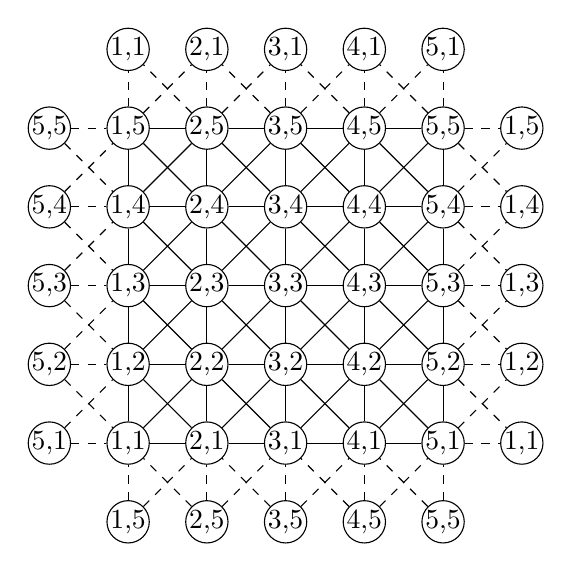
\begin{tikzpicture} 
[
  node distance=0.5cm,
  every node/.style={circle, draw, minimum size=4mm, inner sep=0pt, font = \normalsize},
  every edge/.style={draw, -} 
]

\node[draw=black] (11) at (1,1) {1,1};
\node[draw=black] (12) at (1,2) {1,2};
\node[draw=black] (13) at (1,3) {1,3};
\node[draw=black] (14) at (1,4) {1,4};
\node[draw=black] (15) at (1,5) {1,5};

\node[draw=black] (21) at (2,1) {2,1};
\node[draw=black] (22) at (2,2) {2,2};
\node[draw=black] (23) at (2,3) {2,3};
\node[draw=black] (24) at (2,4) {2,4};
\node[draw=black] (25) at (2,5) {2,5};

\node[draw=black] (31) at (3,1) {3,1};
\node[draw=black] (32) at (3,2) {3,2};
\node[draw=black] (33) at (3,3) {3,3};
\node[draw=black] (34) at (3,4) {3,4};
\node[draw=black] (35) at (3,5) {3,5};

\node[draw=black] (41) at (4,1) {4,1};
\node[draw=black] (42) at (4,2) {4,2};
\node[draw=black] (43) at (4,3) {4,3};
\node[draw=black] (44) at (4,4) {4,4};
\node[draw=black] (45) at (4,5) {4,5};

\node[draw=black] (51) at (5,1) {5,1};
\node[draw=black] (52) at (5,2) {5,2};
\node[draw=black] (53) at (5,3) {5,3};
\node[draw=black] (54) at (5,4) {5,4};
\node[draw=black] (55) at (5,5) {5,5}; 
 

\node[draw=black] (01) at (0,1) {5,1};
\node[draw=black] (02) at (0,2) {5,2};
\node[draw=black] (03) at (0,3) {5,3};
\node[draw=black] (04) at (0,4) {5,4};
\node[draw=black] (05) at (0,5) {5,5};

\node[draw=black] (61) at (6,1) {1,1};
\node[draw=black] (62) at (6,2) {1,2};
\node[draw=black] (63) at (6,3) {1,3};
\node[draw=black] (64) at (6,4) {1,4};
\node[draw=black] (65) at (6,5) {1,5};


\node[draw=black] (10) at (1,0) {1,5};
\node[draw=black] (20) at (2,0) {2,5};
\node[draw=black] (30) at (3,0) {3,5};
\node[draw=black] (40) at (4,0) {4,5};
\node[draw=black] (50) at (5,0) {5,5};

\node[draw=black] (16) at (1,6) {1,1};
\node[draw=black] (26) at (2,6) {2,1};
\node[draw=black] (36) at (3,6) {3,1};
\node[draw=black] (46) at (4,6) {4,1};
\node[draw=black] (56) at (5,6) {5,1};


\draw (11) edge (12);
\draw (12) edge (13);
\draw (13) edge (14);
\draw (14) edge (15);

\draw (21) edge (22);
\draw (22) edge (23);
\draw (23) edge (24);
\draw (24) edge (25);

\draw (31) edge (32);
\draw (32) edge (33);
\draw (33) edge (34);
\draw (34) edge (35);

\draw (41) edge (42);
\draw (42) edge (43);
\draw (43) edge (44);
\draw (44) edge (45);

\draw (51) edge (52);
\draw (52) edge (53);
\draw (53) edge (54);
\draw (54) edge (55);


\draw (11) edge (21);
\draw (21) edge (31);
\draw (31) edge (41);
\draw (41) edge (51);

\draw (12) edge (22);
\draw (22) edge (32);
\draw (32) edge (42);
\draw (42) edge (52);

\draw (13) edge (23);
\draw (23) edge (33);
\draw (33) edge (43);
\draw (43) edge (53);

\draw (14) edge (24);
\draw (24) edge (34);
\draw (34) edge (44);
\draw (44) edge (54);

\draw (15) edge (25);
\draw (25) edge (35);
\draw (35) edge (45);
\draw (45) edge (55);


\draw (11) edge (22);
\draw (21) edge (32);
\draw (31) edge (42);
\draw (41) edge (52);

\draw (12) edge (23);
\draw (22) edge (33);
\draw (32) edge (43);
\draw (42) edge (53);

\draw (13) edge (24);
\draw (23) edge (34);
\draw (33) edge (44);
\draw (43) edge (54);

\draw (14) edge (25);
\draw (24) edge (35);
\draw (34) edge (45);
\draw (44) edge (55); 

 
\draw (21) edge (12);
\draw (31) edge (22);
\draw (41) edge (32);
\draw (51) edge (42);
 
\draw (22) edge (13);
\draw (32) edge (23);
\draw (42) edge (33);
\draw (52) edge (43);
 
\draw (23) edge (14);
\draw (33) edge (24);
\draw (43) edge (34);
\draw (53) edge (44);
 
\draw (24) edge (15);
\draw (34) edge (25);
\draw (44) edge (35);
\draw (54) edge (45);


\draw[dashed] (25) edge (16);
\draw[dashed] (35) edge (26);
\draw[dashed] (45) edge (36);
\draw[dashed] (55) edge (46);

\draw[dashed] (20) edge (11);
\draw[dashed] (30) edge (21);
\draw[dashed] (40) edge (31);
\draw[dashed] (50) edge (41);


\draw[dashed] (10) edge (21);
\draw[dashed] (20) edge (31);
\draw[dashed] (30) edge (41);
\draw[dashed] (40) edge (51);


\draw[dashed] (15) edge (26);
\draw[dashed] (25) edge (36);
\draw[dashed] (35) edge (46);
\draw[dashed] (45) edge (56);




\draw[dashed] (52) edge (61);
\draw[dashed] (53) edge (62);
\draw[dashed] (54) edge (63);
\draw[dashed] (55) edge (64);

\draw[dashed] (02) edge (11);
\draw[dashed] (03) edge (12);
\draw[dashed] (04) edge (13);
\draw[dashed] (05) edge (14);


\draw[dashed] (01) edge (12);
\draw[dashed] (02) edge (13);
\draw[dashed] (03) edge (14);
\draw[dashed] (04) edge (15);


\draw[dashed] (51) edge (62);
\draw[dashed] (52) edge (63);
\draw[dashed] (53) edge (64);
\draw[dashed] (54) edge (65);

\draw[dashed] (51) edge (61);
\draw[dashed] (52) edge (62);
\draw[dashed] (53) edge (63);
\draw[dashed] (54) edge (64);
\draw[dashed] (55) edge (65);

\draw[dashed] (01) edge (11);
\draw[dashed] (02) edge (12);
\draw[dashed] (03) edge (13);
\draw[dashed] (04) edge (14);
\draw[dashed] (05) edge (15);


\draw[dashed] (15) edge (16);
\draw[dashed] (25) edge (26);
\draw[dashed] (35) edge (36);
\draw[dashed] (45) edge (46);
\draw[dashed] (55) edge (56);

\draw[dashed] (10) edge (11);
\draw[dashed] (20) edge (21);
\draw[dashed] (30) edge (31);
\draw[dashed] (40) edge (41);
\draw[dashed] (50) edge (51);
\end{tikzpicture}

    \caption{Two-fold $f$-confusion graphs of $\tilde f$.}
\end{figure}
\begin{figure}[h]
    \centering

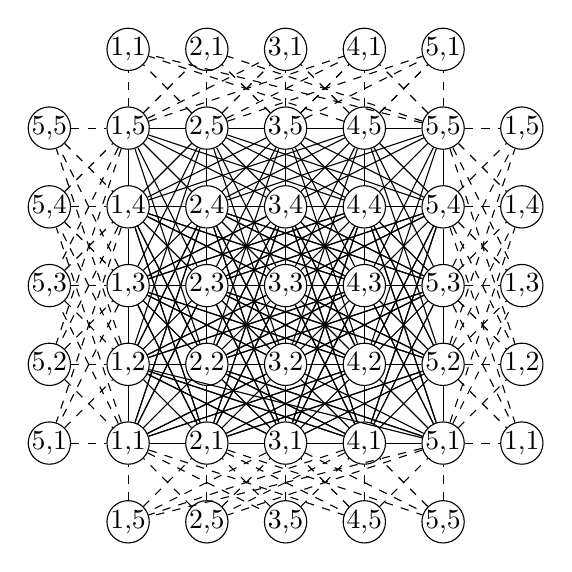
\begin{tikzpicture} 
[
  node distance=0.5cm,
  every node/.style={circle, draw, minimum size=4mm, inner sep=0pt, font = \normalsize},
  every edge/.style={draw, -} 
]

\node[draw=black] (11) at (1,1) {1,1};
\node[draw=black] (12) at (1,2) {1,2};
\node[draw=black] (13) at (1,3) {1,3};
\node[draw=black] (14) at (1,4) {1,4};
\node[draw=black] (15) at (1,5) {1,5};

\node[draw=black] (21) at (2,1) {2,1};
\node[draw=black] (22) at (2,2) {2,2};
\node[draw=black] (23) at (2,3) {2,3};
\node[draw=black] (24) at (2,4) {2,4};
\node[draw=black] (25) at (2,5) {2,5};

\node[draw=black] (31) at (3,1) {3,1};
\node[draw=black] (32) at (3,2) {3,2};
\node[draw=black] (33) at (3,3) {3,3};
\node[draw=black] (34) at (3,4) {3,4};
\node[draw=black] (35) at (3,5) {3,5};

\node[draw=black] (41) at (4,1) {4,1};
\node[draw=black] (42) at (4,2) {4,2};
\node[draw=black] (43) at (4,3) {4,3};
\node[draw=black] (44) at (4,4) {4,4};
\node[draw=black] (45) at (4,5) {4,5};

\node[draw=black] (51) at (5,1) {5,1};
\node[draw=black] (52) at (5,2) {5,2};
\node[draw=black] (53) at (5,3) {5,3};
\node[draw=black] (54) at (5,4) {5,4};
\node[draw=black] (55) at (5,5) {5,5}; 
 

\node[draw=black] (01) at (0,1) {5,1};
\node[draw=black] (02) at (0,2) {5,2};
\node[draw=black] (03) at (0,3) {5,3};
\node[draw=black] (04) at (0,4) {5,4};
\node[draw=black] (05) at (0,5) {5,5};

\node[draw=black] (61) at (6,1) {1,1};
\node[draw=black] (62) at (6,2) {1,2};
\node[draw=black] (63) at (6,3) {1,3};
\node[draw=black] (64) at (6,4) {1,4};
\node[draw=black] (65) at (6,5) {1,5};


\node[draw=black] (10) at (1,0) {1,5};
\node[draw=black] (20) at (2,0) {2,5};
\node[draw=black] (30) at (3,0) {3,5};
\node[draw=black] (40) at (4,0) {4,5};
\node[draw=black] (50) at (5,0) {5,5};

\node[draw=black] (16) at (1,6) {1,1};
\node[draw=black] (26) at (2,6) {2,1};
\node[draw=black] (36) at (3,6) {3,1};
\node[draw=black] (46) at (4,6) {4,1};
\node[draw=black] (56) at (5,6) {5,1};


\draw (11) edge (12);
\draw (12) edge (13);
\draw (13) edge (14);
\draw (14) edge (15);

\draw (21) edge (22);
\draw (22) edge (23);
\draw (23) edge (24);
\draw (24) edge (25);

\draw (31) edge (32);
\draw (32) edge (33);
\draw (33) edge (34);
\draw (34) edge (35);

\draw (41) edge (42);
\draw (42) edge (43);
\draw (43) edge (44);
\draw (44) edge (45);

\draw (51) edge (52);
\draw (52) edge (53);
\draw (53) edge (54);
\draw (54) edge (55);


\draw (11) edge (21);
\draw (21) edge (31);
\draw (31) edge (41);
\draw (41) edge (51);

\draw (12) edge (22);
\draw (22) edge (32);
\draw (32) edge (42);
\draw (42) edge (52);

\draw (13) edge (23);
\draw (23) edge (33);
\draw (33) edge (43);
\draw (43) edge (53);

\draw (14) edge (24);
\draw (24) edge (34);
\draw (34) edge (44);
\draw (44) edge (54);

\draw (15) edge (25);
\draw (25) edge (35);
\draw (35) edge (45);
\draw (45) edge (55);


\draw (11) edge (22);
\draw (21) edge (32);
\draw (31) edge (42);
\draw (41) edge (52);

\draw (12) edge (23);
\draw (22) edge (33);
\draw (32) edge (43);
\draw (42) edge (53);

\draw (13) edge (24);
\draw (23) edge (34);
\draw (33) edge (44);
\draw (43) edge (54);

\draw (14) edge (25);
\draw (24) edge (35);
\draw (34) edge (45);
\draw (44) edge (55); 

 
\draw (21) edge (12);
\draw (31) edge (22);
\draw (41) edge (32);
\draw (51) edge (42);
 
\draw (22) edge (13);
\draw (32) edge (23);
\draw (42) edge (33);
\draw (52) edge (43);
 
\draw (23) edge (14);
\draw (33) edge (24);
\draw (43) edge (34);
\draw (53) edge (44);
 
\draw (24) edge (15);
\draw (34) edge (25);
\draw (44) edge (35);
\draw (54) edge (45);


\draw[dashed] (25) edge (16);
\draw[dashed] (35) edge (26);
\draw[dashed] (45) edge (36);
\draw[dashed] (55) edge (46);

\draw[dashed] (20) edge (11);
\draw[dashed] (30) edge (21);
\draw[dashed] (40) edge (31);
\draw[dashed] (50) edge (41);


\draw[dashed] (10) edge (21);
\draw[dashed] (20) edge (31);
\draw[dashed] (30) edge (41);
\draw[dashed] (40) edge (51);


\draw[dashed] (15) edge (26);
\draw[dashed] (25) edge (36);
\draw[dashed] (35) edge (46);
\draw[dashed] (45) edge (56);




\draw[dashed] (52) edge (61);
\draw[dashed] (53) edge (62);
\draw[dashed] (54) edge (63);
\draw[dashed] (55) edge (64);

\draw[dashed] (02) edge (11);
\draw[dashed] (03) edge (12);
\draw[dashed] (04) edge (13);
\draw[dashed] (05) edge (14);


\draw[dashed] (01) edge (12);
\draw[dashed] (02) edge (13);
\draw[dashed] (03) edge (14);
\draw[dashed] (04) edge (15);


\draw[dashed] (51) edge (62);
\draw[dashed] (52) edge (63);
\draw[dashed] (53) edge (64);
\draw[dashed] (54) edge (65);

\draw[dashed] (51) edge (61);
\draw[dashed] (52) edge (62);
\draw[dashed] (53) edge (63);
\draw[dashed] (54) edge (64);
\draw[dashed] (55) edge (65);

\draw[dashed] (01) edge (11);
\draw[dashed] (02) edge (12);
\draw[dashed] (03) edge (13);
\draw[dashed] (04) edge (14);
\draw[dashed] (05) edge (15);


\draw[dashed] (15) edge (16);
\draw[dashed] (25) edge (26);
\draw[dashed] (35) edge (36);
\draw[dashed] (45) edge (46);
\draw[dashed] (55) edge (56);

\draw[dashed] (10) edge (11);
\draw[dashed] (20) edge (21);
\draw[dashed] (30) edge (31);
\draw[dashed] (40) edge (41);
\draw[dashed] (50) edge (51);



\draw (11) edge (32);
\draw (11) edge (42);
\draw (11) edge (23);
\draw (11) edge (24);

\draw[dashed] (11) edge (30);
\draw[dashed] (11) edge (40);
\draw[dashed] (11) edge (04);
\draw[dashed] (11) edge (03);


\draw (21) edge (33);
\draw (21) edge (34);
\draw (21) edge (13);
\draw (21) edge (14);

\draw (21) edge (52);
\draw (21) edge (42);
\draw[dashed] (21) edge (50);
\draw[dashed] (21) edge (40);


\draw (31) edge (43);
\draw (31) edge (44);
\draw (31) edge (23);
\draw (31) edge (24);

\draw (31) edge (12);
\draw (31) edge (52);
\draw[dashed] (31) edge (10);
\draw[dashed] (31) edge (50);


\draw (41) edge (53);
\draw (41) edge (54);
\draw (41) edge (33);
\draw (41) edge (34);

\draw (41) edge (12);
\draw (41) edge (22);
\draw[dashed] (41) edge (10);
\draw[dashed] (41) edge (20);

\draw (51) edge (43);
\draw (51) edge (44);
\draw[dashed] (51) edge (63);
\draw[dashed] (51) edge (64);

\draw (51) edge (12);
\draw (51) edge (22);
\draw[dashed] (51) edge (10);
\draw[dashed] (51) edge (20);

%--------------------
\draw (12) edge (31);
\draw (12) edge (41);
\draw (12) edge (33);
\draw (12) edge (43);

\draw (12) edge (24);
\draw (12) edge (25);
\draw[dashed] (12) edge (04);
\draw[dashed] (12) edge (05);


\draw (22) edge (41);
\draw (22) edge (51);
\draw (22) edge (43);
\draw (22) edge (53);

\draw (22) edge (14);
\draw (22) edge (15);
\draw (22) edge (34);
\draw (22) edge (35);


\draw (32) edge (51);
\draw (32) edge (11);
\draw (32) edge (53);
\draw (32) edge (13);

\draw (32) edge (24);
\draw (32) edge (25);
\draw (32) edge (44);
\draw (32) edge (45);



\draw (42) edge (21);
\draw (42) edge (11);
\draw (42) edge (23);
\draw (42) edge (13);

\draw (42) edge (34);
\draw (42) edge (35);
\draw (42) edge (54);
\draw (42) edge (55);


\draw (52) edge (31);
\draw (52) edge (21);
\draw (52) edge (33);
\draw (52) edge (23);

\draw (52) edge (44);
\draw (52) edge (45);
\draw[dashed] (52) edge (64);
\draw[dashed] (52) edge (65);
%---------------

%--------------------
\draw (13) edge (32);
\draw (13) edge (42);
\draw (13) edge (34);
\draw (13) edge (44);

\draw (13) edge (25);
\draw (13) edge (21);
\draw[dashed] (13) edge (05);
\draw[dashed] (13) edge (01);


\draw (23) edge (42);
\draw (23) edge (52);
\draw (23) edge (44);
\draw (23) edge (54);

\draw (23) edge (15);
\draw (23) edge (11);
\draw (23) edge (35);
\draw (23) edge (31);


\draw (33) edge (52);
\draw (33) edge (12);
\draw (33) edge (54);
\draw (33) edge (14);

\draw (33) edge (25);
\draw (33) edge (21);
\draw (33) edge (45);
\draw (33) edge (41);



\draw (43) edge (22);
\draw (43) edge (12);
\draw (43) edge (24);
\draw (43) edge (14);

\draw (43) edge (35);
\draw (43) edge (31);
\draw (43) edge (55);
\draw (43) edge (51);


\draw (53) edge (32);
\draw (53) edge (22);
\draw (53) edge (34);
\draw (53) edge (24);

\draw (53) edge (45);
\draw (53) edge (41);
\draw[dashed] (53) edge (65);
\draw[dashed] (53) edge (61);
%---------------


%--------------------
\draw (14) edge (33);
\draw (14) edge (43);
\draw (14) edge (35);
\draw (14) edge (45);

\draw (14) edge (22);
\draw (14) edge (21);
\draw[dashed] (14) edge (02);
\draw[dashed] (14) edge (01);


\draw (24) edge (43);
\draw (24) edge (53);
\draw (24) edge (45);
\draw (24) edge (55);

\draw (24) edge (12);
\draw (24) edge (11);
\draw (24) edge (32);
\draw (24) edge (31);


\draw (34) edge (53);
\draw (34) edge (13);
\draw (34) edge (55);
\draw (34) edge (15);

\draw (34) edge (22);
\draw (34) edge (21);
\draw (34) edge (42);
\draw (34) edge (41);



\draw (44) edge (23);
\draw (44) edge (13);
\draw (44) edge (25);
\draw (44) edge (15);

\draw (44) edge (32);
\draw (44) edge (31);
\draw (44) edge (52);
\draw (44) edge (51);


\draw (54) edge (33);
\draw (54) edge (23);
\draw (54) edge (35);
\draw (54) edge (25);

\draw (54) edge (42);
\draw (54) edge (41);
\draw[dashed] (54) edge (62);
\draw[dashed] (54) edge (61);
%---------------


\draw[dashed] (15) edge (02);
\draw[dashed] (15) edge (03); 

\draw[dashed] (55) edge (62);
\draw[dashed] (55) edge (63); 



\draw[dashed] (15) edge (46);
\draw[dashed] (15) edge (36); 

\draw[dashed] (25) edge (56);
\draw[dashed] (25) edge (46); 

\draw[dashed] (35) edge (56);
\draw[dashed] (35) edge (46); 

\draw[dashed] (45) edge (16);
\draw[dashed] (45) edge (56); 

\draw[dashed] (55) edge (16);
\draw[dashed] (55) edge (26); 6+2+6

\end{tikzpicture}

    \caption{Two-fold $f$-confusion graphs of $\tilde g$.}
\end{figure}
\begin{figure}[h]
    \centering

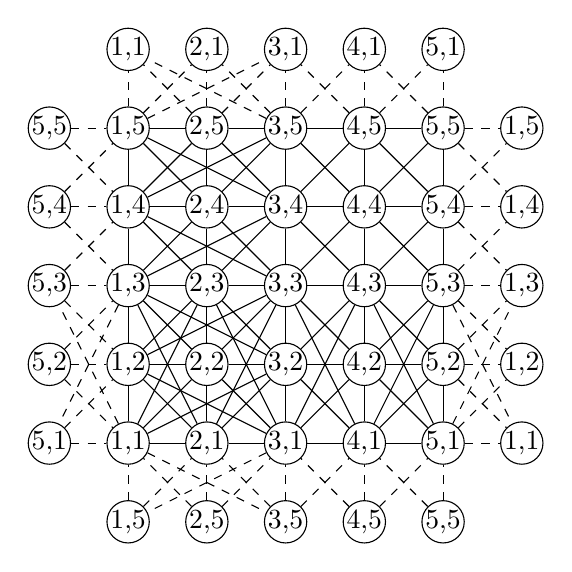
\begin{tikzpicture} 
[
  node distance=0.5cm,
  every node/.style={circle, draw, minimum size=4mm, inner sep=0pt, font = \normalsize},
  every edge/.style={draw, -} 
]

\node[draw=black] (11) at (1,1) {1,1};
\node[draw=black] (12) at (1,2) {1,2};
\node[draw=black] (13) at (1,3) {1,3};
\node[draw=black] (14) at (1,4) {1,4};
\node[draw=black] (15) at (1,5) {1,5};

\node[draw=black] (21) at (2,1) {2,1};
\node[draw=black] (22) at (2,2) {2,2};
\node[draw=black] (23) at (2,3) {2,3};
\node[draw=black] (24) at (2,4) {2,4};
\node[draw=black] (25) at (2,5) {2,5};

\node[draw=black] (31) at (3,1) {3,1};
\node[draw=black] (32) at (3,2) {3,2};
\node[draw=black] (33) at (3,3) {3,3};
\node[draw=black] (34) at (3,4) {3,4};
\node[draw=black] (35) at (3,5) {3,5};

\node[draw=black] (41) at (4,1) {4,1};
\node[draw=black] (42) at (4,2) {4,2};
\node[draw=black] (43) at (4,3) {4,3};
\node[draw=black] (44) at (4,4) {4,4};
\node[draw=black] (45) at (4,5) {4,5};

\node[draw=black] (51) at (5,1) {5,1};
\node[draw=black] (52) at (5,2) {5,2};
\node[draw=black] (53) at (5,3) {5,3};
\node[draw=black] (54) at (5,4) {5,4};
\node[draw=black] (55) at (5,5) {5,5}; 
 

\node[draw=black] (01) at (0,1) {5,1};
\node[draw=black] (02) at (0,2) {5,2};
\node[draw=black] (03) at (0,3) {5,3};
\node[draw=black] (04) at (0,4) {5,4};
\node[draw=black] (05) at (0,5) {5,5};

\node[draw=black] (61) at (6,1) {1,1};
\node[draw=black] (62) at (6,2) {1,2};
\node[draw=black] (63) at (6,3) {1,3};
\node[draw=black] (64) at (6,4) {1,4};
\node[draw=black] (65) at (6,5) {1,5};


\node[draw=black] (10) at (1,0) {1,5};
\node[draw=black] (20) at (2,0) {2,5};
\node[draw=black] (30) at (3,0) {3,5};
\node[draw=black] (40) at (4,0) {4,5};
\node[draw=black] (50) at (5,0) {5,5};

\node[draw=black] (16) at (1,6) {1,1};
\node[draw=black] (26) at (2,6) {2,1};
\node[draw=black] (36) at (3,6) {3,1};
\node[draw=black] (46) at (4,6) {4,1};
\node[draw=black] (56) at (5,6) {5,1};


\draw (11) edge (12);
\draw (12) edge (13);
\draw (13) edge (14);
\draw (14) edge (15);

\draw (21) edge (22);
\draw (22) edge (23);
\draw (23) edge (24);
\draw (24) edge (25);

\draw (31) edge (32);
\draw (32) edge (33);
\draw (33) edge (34);
\draw (34) edge (35);

\draw (41) edge (42);
\draw (42) edge (43);
\draw (43) edge (44);
\draw (44) edge (45);

\draw (51) edge (52);
\draw (52) edge (53);
\draw (53) edge (54);
\draw (54) edge (55);


\draw (11) edge (21);
\draw (21) edge (31);
\draw (31) edge (41);
\draw (41) edge (51);

\draw (12) edge (22);
\draw (22) edge (32);
\draw (32) edge (42);
\draw (42) edge (52);

\draw (13) edge (23);
\draw (23) edge (33);
\draw (33) edge (43);
\draw (43) edge (53);

\draw (14) edge (24);
\draw (24) edge (34);
\draw (34) edge (44);
\draw (44) edge (54);

\draw (15) edge (25);
\draw (25) edge (35);
\draw (35) edge (45);
\draw (45) edge (55);


\draw (11) edge (22);
\draw (21) edge (32);
\draw (31) edge (42);
\draw (41) edge (52);

\draw (12) edge (23);
\draw (22) edge (33);
\draw (32) edge (43);
\draw (42) edge (53);

\draw (13) edge (24);
\draw (23) edge (34);
\draw (33) edge (44);
\draw (43) edge (54);

\draw (14) edge (25);
\draw (24) edge (35);
\draw (34) edge (45);
\draw (44) edge (55); 

 
\draw (21) edge (12);
\draw (31) edge (22);
\draw (41) edge (32);
\draw (51) edge (42);
 
\draw (22) edge (13);
\draw (32) edge (23);
\draw (42) edge (33);
\draw (52) edge (43);
 
\draw (23) edge (14);
\draw (33) edge (24);
\draw (43) edge (34);
\draw (53) edge (44);
 
\draw (24) edge (15);
\draw (34) edge (25);
\draw (44) edge (35);
\draw (54) edge (45);


\draw[dashed] (25) edge (16);
\draw[dashed] (35) edge (26);
\draw[dashed] (45) edge (36);
\draw[dashed] (55) edge (46);

\draw[dashed] (20) edge (11);
\draw[dashed] (30) edge (21);
\draw[dashed] (40) edge (31);
\draw[dashed] (50) edge (41);


\draw[dashed] (10) edge (21);
\draw[dashed] (20) edge (31);
\draw[dashed] (30) edge (41);
\draw[dashed] (40) edge (51);


\draw[dashed] (15) edge (26);
\draw[dashed] (25) edge (36);
\draw[dashed] (35) edge (46);
\draw[dashed] (45) edge (56);




\draw[dashed] (52) edge (61);
\draw[dashed] (53) edge (62);
\draw[dashed] (54) edge (63);
\draw[dashed] (55) edge (64);

\draw[dashed] (02) edge (11);
\draw[dashed] (03) edge (12);
\draw[dashed] (04) edge (13);
\draw[dashed] (05) edge (14);


\draw[dashed] (01) edge (12);
\draw[dashed] (02) edge (13);
\draw[dashed] (03) edge (14);
\draw[dashed] (04) edge (15);


\draw[dashed] (51) edge (62);
\draw[dashed] (52) edge (63);
\draw[dashed] (53) edge (64);
\draw[dashed] (54) edge (65);

\draw[dashed] (51) edge (61);
\draw[dashed] (52) edge (62);
\draw[dashed] (53) edge (63);
\draw[dashed] (54) edge (64);
\draw[dashed] (55) edge (65);

\draw[dashed] (01) edge (11);
\draw[dashed] (02) edge (12);
\draw[dashed] (03) edge (13);
\draw[dashed] (04) edge (14);
\draw[dashed] (05) edge (15);


\draw[dashed] (15) edge (16);
\draw[dashed] (25) edge (26);
\draw[dashed] (35) edge (36);
\draw[dashed] (45) edge (46);
\draw[dashed] (55) edge (56);

\draw[dashed] (10) edge (11);
\draw[dashed] (20) edge (21);
\draw[dashed] (30) edge (31);
\draw[dashed] (40) edge (41);
\draw[dashed] (50) edge (51);


\draw[dashed] (11) edge (03);
\draw[dashed] (11) edge (30);
\draw[dashed] (53) edge (61);
\draw[dashed] (35) edge (16);
\draw (11) edge (23);
\draw (11) edge (32);

\draw (21) edge (33);
\draw (31) edge (43);
\draw (31) edge (23);
\draw (41) edge (53);
\draw (41) edge (33);
\draw (51) edge (43);
\draw[dashed] (51) edge (63);


\draw (12) edge (33);
\draw (12) edge (31);



\draw[dashed] (13) edge (01); 
\draw (13) edge (21);
\draw (13) edge (32);
\draw (13) edge (34);
 
\draw (33) edge (14); 
 
\draw (14) edge (35); 
\draw (15) edge (34); 
\draw[dashed] (15) edge (36); 
\draw[dashed] (31) edge (10); 


\end{tikzpicture}

    \caption{Two-fold $f$-confusion graphs of $\tilde h$.}
\end{figure}

\end{document}

\textbf{}
